\documentclass[reprint,amsmath,amssymb,aps,pre,showkeys,showpacs]{revtex4-1}
\usepackage[english]{babel}
\usepackage[utf8]{inputenc}
\usepackage[T1]{fontenc}
\usepackage{bm}
\usepackage{xcolor}
\usepackage{algpseudocode}
\usepackage{graphicx}
\usepackage{subfigure}
\usepackage[export]{adjustbox}
\usepackage{hyperref}
\usepackage{cleveref}
\usepackage[inline]{enumitem}
\usepackage{resizegather}

\definecolor{light-gray}{gray}{0.95}
\newcommand{\code}[1]{\colorbox{light-gray}{\texttt{#1}}}

\begin{document}
\preprint{APS/123-QED}

\author{Vasily Postnicov\textsuperscript{1}}
\author{Marina V. Karsanina\textsuperscript{1}}
\author{Aleksey Khlyupin\textsuperscript{1}}
\author{Kirill M. Gerke\textsuperscript{1}}
\email{kg@ifz.ru}

\affiliation{\textsuperscript{1}Schmidt Institute of Physics of the Earth of
  Russian Academy of Sciences, Moscow, 107031, Russia}
%\affiliation{\textsuperscript{2}Computational Mathematics and Cybernetics,
%  Lomonosov Moscow State University, Moscow, 119991, Russia}
%\affiliation{\textsuperscript{3}Oil and Gas Research Institute Russian Academy
%  of Sciences (OGRI RAS) 3, Gubkina st., Moscow, 119333, Russian Federation}

\title{Surface correlation functions calculations: improving methodology for
  discrete images with novel exact continuous approach}

\begin{abstract}
  Here we are again.
\end{abstract}
\keywords {3D images; correlation functions; surface-surface function;
  surface-void function; image analysis; image scaling}

\maketitle

\section{Introduction}
\label{sec:intro}
Correlation functions (CFs) to describe structures arose from scattering
experiments \cite{debye1957scattering} and found their way into numerous
disciplines and applications: from material sciences
\cite{Cecen,chen2022quantifying}, to rock \cite{ledesma2018effect} and soil
physics \cite{Euras2012,PLoS_ONE,KarsaninaEJSS}, cosmology \cite{TakadaJain} and
food engineering \cite{Derossi2019}. In particular, correlation functions as
computed from structural images were used for:
\begin{enumerate}
  \item characterization of morphology \cite{tensorPRE} and representativeness
    via correlation lengths \cite{vcapek2011transport,thovert2011grain} at which
    CFs reach plateau;
  \item comparison of different structures \cite{jiao2014chawla,EPL1,REVpaper},
    usually by computing L-2 norm difference between CFs for two or more images,
  \item compressing structural information \cite{SciRep1,Havelka} by
    representing huge datasets in the form of a limited set of CFs that can be
    further squeezed into parameters for a number of basis functions
    \cite{jiao_basis,KarsaninaEJSS},
  \item describing structural dynamics and evolution
    \cite{chen2015dynamic,PLoS_ONE,xu2022correlation},
  \item extracting features for deep learning
    \cite{Miao2017,kamrava2020linking,roding2020predicting,KarsaninaEJSS},
  \item performing stochastic reconstructions
    \cite{Adler_recon,Y-T,EPL2,tahmasebiPRL,karsaninaPRL} based on limited input
    data such as, for example, CFs obtained from 2D cuts,
  \item fusing multi-scale images \cite{SciRep1,chen2016stochastic,Geoderma2018}
    into a single representation,
  \item evaluation of image replica quality, e.g., stochastic reconstructions
    \cite{deeep_papers_or_somethingelse},
  \item assessing stationarity of the structure at hand \cite{REVpaper}.
\end{enumerate}

In majority, if not all, cases mentioned above, surface functions - namely,
$F_{ss}$ and $F_{sv}$ - were underrepresented due to our inability to compute
them in a robust way. While known for a long time \cite{theory_in_MT}, only
somewhat crude approximate approaches \cite{crude_approx_inMT} were developed
until Ma and Torquato laid foundation for such a robust computational
methodology \cite{ma2018SS}. They proposed an elegant solution for infinite
resolution Gaussian random fields, or "continouos" approach. They also assumed
that the same approach can be readily applied to discrete experimental images if
grey-scale values are thresholded in a similar way to continuious Gaussian
field. Samarin et al. \cite{our_SS_paper} argued that experimental images needs
to be segmented first using current cutting edge techniques \cite{NNseg} and
proposed "discrete" approach. The latter allowed to obtain surface functions
closer to analytical solutions for overlapping disks/spheres and to supress
noise, in particular for $F_{ss}$. The noise in Ma and Torquato method resulted
from $1/cos(\theta)$ computations during random line segment placement - this
leaves a room for improvements. While Samarin et al. obtained better convergence
with analytical solution, this was demostrated only for overlapping disks image
of limited size (that can potentially introduce some differences between
computations and analytical solution for infinite size structure). Moreover,
good agreement was achieved by manually fitting the values of edge-detecting
filter that could lack accuracy for arbitrary structure different from
overlapping disks. In other words, we still lack robustness in surface CFs
evaluation due to inability to directly compare "discrete" versus "continuous"
methodology, and verify both approaches for arbitrary geometries.

If computed accurately for any arbitrary structure at hand, surface CFs can be
utilized in a multitude of applications:
\begin{enumerate}
  \item describing real surfaces resulting from different mechanical processes,
    e.g., cracking \cite{some_examples},
  \item delineating surface evolution \cite{chen2022} during such mechanical
    cracking events or reactive transport in porous media
    \cite{godinho2016,noiriel2021,prokhorov2022},
  \item representing surface features in super-resolution and stochastic
    reconstruction techniques \cite{chen2020super,janssens2020,karimpouli2022}.
\end{enumerate}
The examples above a just a few potential applications that, due to ability for
surface CFs to establish themselves as universal interface/surface descriptors,
highlight the necessity to establish robust techniques for $F_{ss}$ and $F_{sv}$
evaluation.

In this contribution we continue to build upon foundational work of Ma and
Torquato \cite{ma2018SS} and recent findings of Samarin et al. \cite{our_SS} to
develop a robust and efficient approach to compute surface correlation functions
from digital 2D and 3D images. In partiuclar, here our aim is to establish a
direct verification of "discrete" methodology (that is easily parallelizable on
CPU and GPU architectures) using exact noiseless "continuous" approach for
arbitrary structures (still described by some continuous function). The rest of
the manuscript is organized as follows: in \cref{sec:def} we introduce some
major definitions of CFs necessary for establishing algorithms, in
\cref{sec:algo} we describe the all methodological details for "discrete" method
for digital images. Next, in \cref{sec:algo-precise} we explain in detail why
verification of computational approaches for digital images is currently
hampered, and then introduce novel exact "continuous" methodology in
\cref{sec:fss-2d}. The choice of verification cases is presented in
\cref{sec:results} followed by improvements in methodology of Samarin et~al. The
paper concludes with discussion, outline and summary in \cref{sec:summary}.

\section{Definitions}
\label{sec:def}
Let $A$ be a set in Euclidean space $\mathbb{R}^n$. A function
$\chi_A(\mathbf{x})$ is called an indicator function for the set $A$ and is
defined as follows:
\begin{equation*}
  \chi_A(\bm{x}) = \left\{
  \begin{array}{ll}
    1 & \quad \bm{x} \in A \\
    0 & \quad \text{otherwise}
  \end{array}
  \right.
\end{equation*}

Now we define two disjoint sets in a homogeneous porous medium: a set of solid
phase $S$ and a set of void phase $V$. Surface-surface correlation function
$F_{ss}$ and surface-void correlation function $F_{sv}$ are then defined as follows:
\begin{align}
  F_{ss}(\bm{r}) &= \langle |\nabla \chi_S(\bm{x})| |\nabla \chi_S(\bm{x} +
  \bm{r})| \rangle \label{eq:fss} \\
  F_{sv}(\bm{r}) &= \langle |\nabla \chi_S(\bm{x})| \chi_V(\bm{x} +
  \bm{r}) \rangle \label{eq:fsv}
\end{align}
Here the brackets $\langle \dots \rangle$ denote ensemble average. If the medium
under consideration is also isotropic, the argument in functions $F_{ss}$ and
$F_{sv}$ can be replaced with a scalar $r = |\bm{r}|$:
\begin{align*}
  F_{ss}(r) &= F_{ss}(\bm{r}) \\
  F_{sv}(r) &= F_{sv}(\bm{r})
\end{align*}
In case correlation functions are computed in predefined directions, scalar
values can be also used for anisotropic structures
\cite{jiao2014chawla,EPL1}. These functions are defined for media with
dimensionality of 2 and higher. $F_{sv}$ is a physical quantity inversely
proportional to length and $F_{ss}$ is inversionaly proportional to surface
area. SI units of measurement for these functions are $m^{-1}$ for $F_{sv}$
and $m^{-2}$ for $F_{ss}$. In practice non-standard units of measurement can be
used instead.

Another function studied in this paper is surface-surface-surface function
$F_{sss}$. It is defined as follows:
\begin{equation}
  F_{sss}(\bm{r_1}, \bm{r_2}) = \langle |\nabla \chi_S(\bm{x})|
  |\nabla \chi_S(\bm{x} + \bm{r_1})|
  |\nabla \chi_S(\bm{x} + \bm{r_2})|
  \rangle \label{eq:fsss}
\end{equation}
This function is defined for media with dimensionality 3 or higher and is a
physical quantity inversely proportional to volume. SI units for $F_{sss}$ are
$m^{-3}$ but other units can be used in practice. For three-dimensional media
$F_{sss}$ is a function of six scalar arguments:
$\bm{r_1} = (r_{1x}, r_{1y}, r_{1z})$ and $\bm{r_2} = (r_{2x}, r_{2y}, r_{2z})$.
However if the medium under consideration is isotropic, only three scalar
arguments $r_1 = |\bm{r_1}|$, $r_2 = |\bm{r_2}|$ and $r_3 = |\bm{r_1} - \bm{r_2}|$
are required. The last argument can be replaced with an angle $\theta$ between
vectors $\bm{r_1}$ and $\bm{r_2}$:
\begin{equation*}
  F_{sss}(r_1, r_2, r_3) = F_{sss}(r_1, r_2, \theta) = F_{sss}(\bm{r_1}, \bm{r_2})
\end{equation*}


More detailed information on surface correlation functions can be found in
\cref{sec:algo-precise} and comprehensive Torquato's book \cite{Torquato_book}.

\section{Computation of surface functions for digital images}
\label{sec:algo}
Here we briefly describe an algorithm for computation of surface-surface,
surface-void and surface-surface-surface correlation functions for digital
images of porous media. A more detailed description can be found in a paper of
Samarin et~al. \textcolor{red}{cite paper} This algorithm can calculate surface
correlation functions for all possible directions and correlation lengths. It
consists of two stages: edge detection stage and computation of autocorrelation.

We give an image of porous medium in the form of two- or three-dimensional bit
array $A$ as the input to our algorithm. In the first stage, we convolve the
input with high-pass filter to extract edges from the image. We use the
following filter kernel $H$:
\begin{equation}
  \begin{aligned}
    H_{ij} &= \frac{1}{6} \left[
      \begin{array}{ccc}
        1 & 1 & 1 \\
        1 & -8 & 1 \\
        1 & 1 & 1
      \end{array}
      \right] \\
    H_{ijk} &= \frac{1}{18} \left[
      \begin{array}{ccc}
        1 & 1 & 1 \\
        1 & 1 & 1 \\
        1 & 1 & 1
      \end{array} ;
      \begin{array}{ccc}
        1 & 1 & 1 \\
        1 & -24 & 1 \\
        1 & 1 & 1
      \end{array} ;
      \begin{array}{ccc}
        1 & 1 & 1 \\
        1 & 1 & 1 \\
        1 & 1 & 1
      \end{array}
      \right]
  \end{aligned}
  \label{eq:filter-3x3}
\end{equation}
Here symbol $;$ denotes concatenation along the third dimension. Edge extraction
is performed as follows:
\begin{align*}
  A'_{lm}  &= \left| \sum_i\sum_j A_{l-i, m-j}H_{ij} \right| \quad \text{for 2D} \\
  A'_{lmn} &= \left| \sum_i\sum_j\sum_k A_{l-i, m-j, n-k}H_{ijk} \right| \quad
  \text{for 3D}
\end{align*}
Therefore $A'$ has non-zero elements only in a small area around interface
between phases in $A$. This operation is convolution of a filter $H$ with an
image $A$ and can be performed using Fourier transform:
\begin{equation*}
  A' = |H*A| = |F^{-1}[F[H] F[A]]|
\end{equation*}
Here $F$ is a forward Fourier transform and $F^{-1}$ is its inverse.

In the second stage we calculate autocorrelation for $A'$ and divide it by a
total number of elements in $A$:
\begin{align*}
  F_{{ss}_{lm}} &= \frac{1}{N} \sum_i \sum_j A'_{ij}A'_{i+l, j+m} \quad
  \text{for 2D} \\
  F_{{ss}_{lmn}} &= \frac{1}{N} \sum_i \sum_j \sum_k A'_{ijk}A'_{i+l, j+m, k+n}
  \quad \text{for 3D}
\end{align*}
Calculation of sums in the latter equations can be performed using the following
properties of Fourier transform (here $\hat{f}(z) = F[f(x)]$):
\begin{equation*}
  F[f(x) \star f(x)] = F[f(x) * f(-x)] = \hat{f}(z)\overline{\hat{f}(z)} = |\hat{f}(z)|^2
\end{equation*}

All in all we get the following algorithm for calculation of $F_{ss}$ function:
\begin{algorithmic}[1]
  \Procedure{surfsurf}{$A$}
  \State $A' \gets |H*A|$
  \Comment{$A'$ becomes an interface of $A$.}
  \State $\hat{A'} \gets F[A']$
  \Comment{Apply DFT to $A'$.}
  \State \textbf{return} $F^{-1}[ |\hat{A}|^2 / N]$
  \Comment{$N$ is a number of elements in $A$}
  \EndProcedure
\end{algorithmic}

Algorithm for surface-void function $F_{sv}$ is similar:
\begin{algorithmic}[1]
  \Procedure{surfvoid}{$A$}
  \State $A' \gets |H*A|$
  \Comment{$A'$ becomes an interface of $A$.}
  \State $V \gets \chi_V(A)$
  \Comment{Apply an indicator function for void phase element-wise to $A$.}
  \State $\hat{A'} \gets F[A']$
  \Comment{Apply DFT to $A'$.}
  \State $\hat{V} \gets F[V]$
  \Comment{Apply DFT to $V$.}
  \State \textbf{return} $F^{-1}[ \hat{A}\overline{\hat{V}} / N]$
  \Comment{$N$ is a number of elements in $A$}
  \EndProcedure
\end{algorithmic}

A result $R_{ij}$ (resp. $R_{ijk}$) of either of two algorithms is an array of
the same shape as $A$ which contains values of correlation function for the
vector $r = (i, j)$ (resp. $r = (i, j, k)$). This result can be averaged over
all directions if needed.

For surface-surface-surface function $F_{sss}$ the former approach can also be
used, but it would be highly inefficient memory-wise because for three
dimensional case $F_{sss}$ is a function of six scalar coordinates which leads
to a very large output array. Instead of this approach we use a slower approach
which computes $F_{sss}$ at a specified point calculating a convolution using
its definition:
\begin{algorithmic}[1]
  \Procedure{surfsurfsurf}{$A$, $\bm{r_1}$, $\bm{r_2}$}
  \State $A' \gets |H*A|$
  \Comment{$A'$ becomes an interface of $A$.}
  \State $A'_1 \gets shift(A', \bm{r_1})$
  \Comment{Shift $A$ in $i$-th dimension by $r_{1i}$ for all $i \in \overline{1, ndim(A)}$}
  \State $A'_2 \gets shift(A', \bm{r_2})$
  \Comment{Shift $A$ in $i$-th dimension by $r_{2i}$ for all $i \in \overline{1, ndim(A)}$}
  \State $M \gets A' \cdot A'_1 \cdot A'_2$
  \Comment{Multiplicate three arrays element-wise}
  \State \textbf{return} $\sum_{i} M_{i} / N$
  \Comment{Sum all elements in $M$ and divide by a number of elements in $A$}
  \EndProcedure
\end{algorithmic}
This algorithm can be vectorized and therefore benefits from the usage of
GPUs. Shift function in this algorithm must be a circular shift which
``rotates'' content of the array, if periodic boundary conditions are
desired. For our purpose we use $F_{sss}$ function in the form
$F_{sss}(r_1, r_2, \theta)$ and fix $\theta = \pi/2$. This leads us to a
sampling pattern shown on \cref{fig:Fsss-pattern}
\begin{figure}
  \centering
  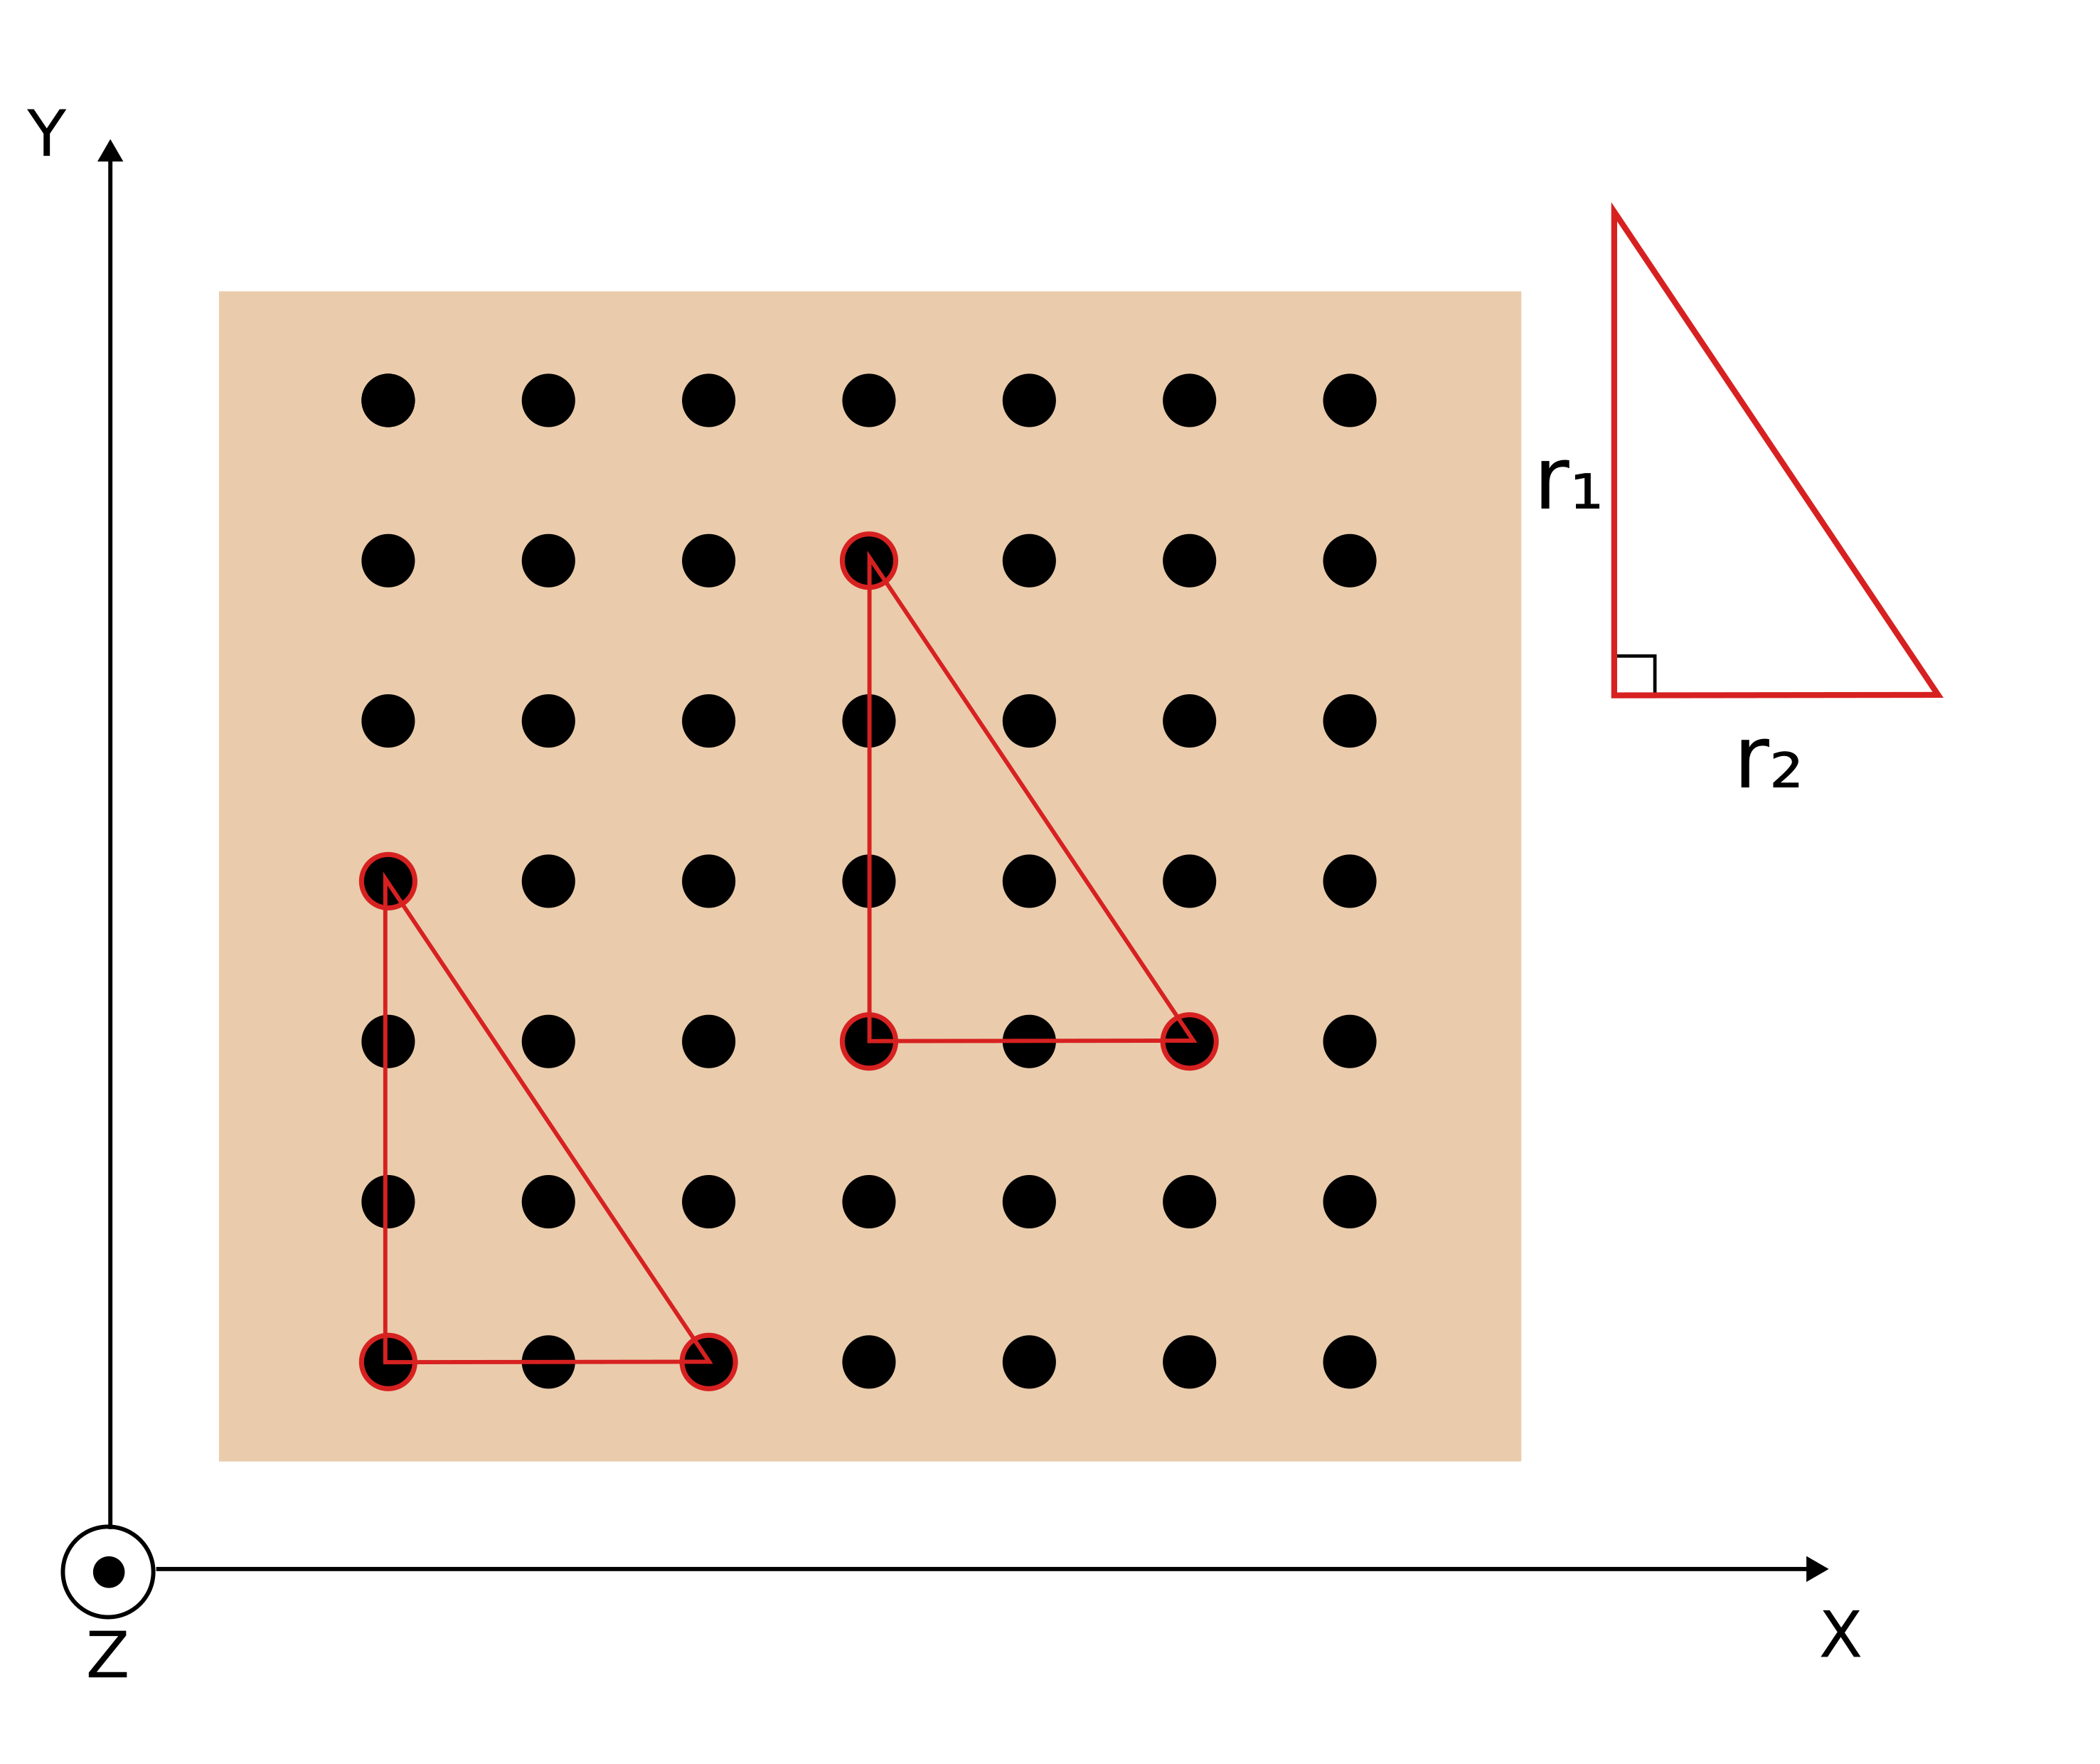
\includegraphics[width=0.8\linewidth]{images/pattern.png}
  \caption[]{Sampling pattern used for calculation of $F_{sss}$ in our
    implementation is a right triangle with fixed catets $r_1$ and $r_2$.
    Patterns can lie in planes $XY$ (as on the picture), $XZ$ or $YZ$. This
    pattern is moved over the input which results in all possible distinct
    configurations. Black dots depict elements of $A'$.}
  \label{fig:Fsss-pattern}
\end{figure}

In addition to filter $H$ we propose an improved filter $H'$. The rationale
behind this improvement is that
\begin{enumerate*}[label=\alph*)]
\item A filter of width 3 is too narrow to give a good approximation for surface
  functions.
\item Filter $H$ is not invariant under rotations, i.e.
  $H*\phi(A) \ne \phi(H*A)$ where $\phi$ is a rotation operator.
\end{enumerate*}
Filter $H'$ has a length $7$ and all coefficients with exception of the central
coefficient are inversely proportional to the distance from the center:
\begin{equation}
  \begin{aligned}
    H'_{ij} &= S \left\{
    \begin{array}{cc}
      \frac{1}{\sqrt{(i-3)^2 + (j-3)^2}} & \quad i \ne 3, j \ne 3 \\
      C & \quad \text{otherwise}
    \end{array}
    \right. \\
    H'_{ijk} &= S \left\{
    \begin{array}{cc}
      \frac{1}{\sqrt{(i-3)^2 + (j-3)^2 + (k-3)^3}} & \quad i \ne 3, j \ne 3, k
      \ne 3 \\
      C & \quad \text{otherwise}
    \end{array}
    \right.
  \end{aligned}
  \label{eq:filter-7x7}
\end{equation}
where $C$ is such that all coefficients of $H'$ sum to zero, and $S$ equals to
$30.45849$ in 2D and $172.96232$ in 3D case.

\begin{figure}
  \centering
  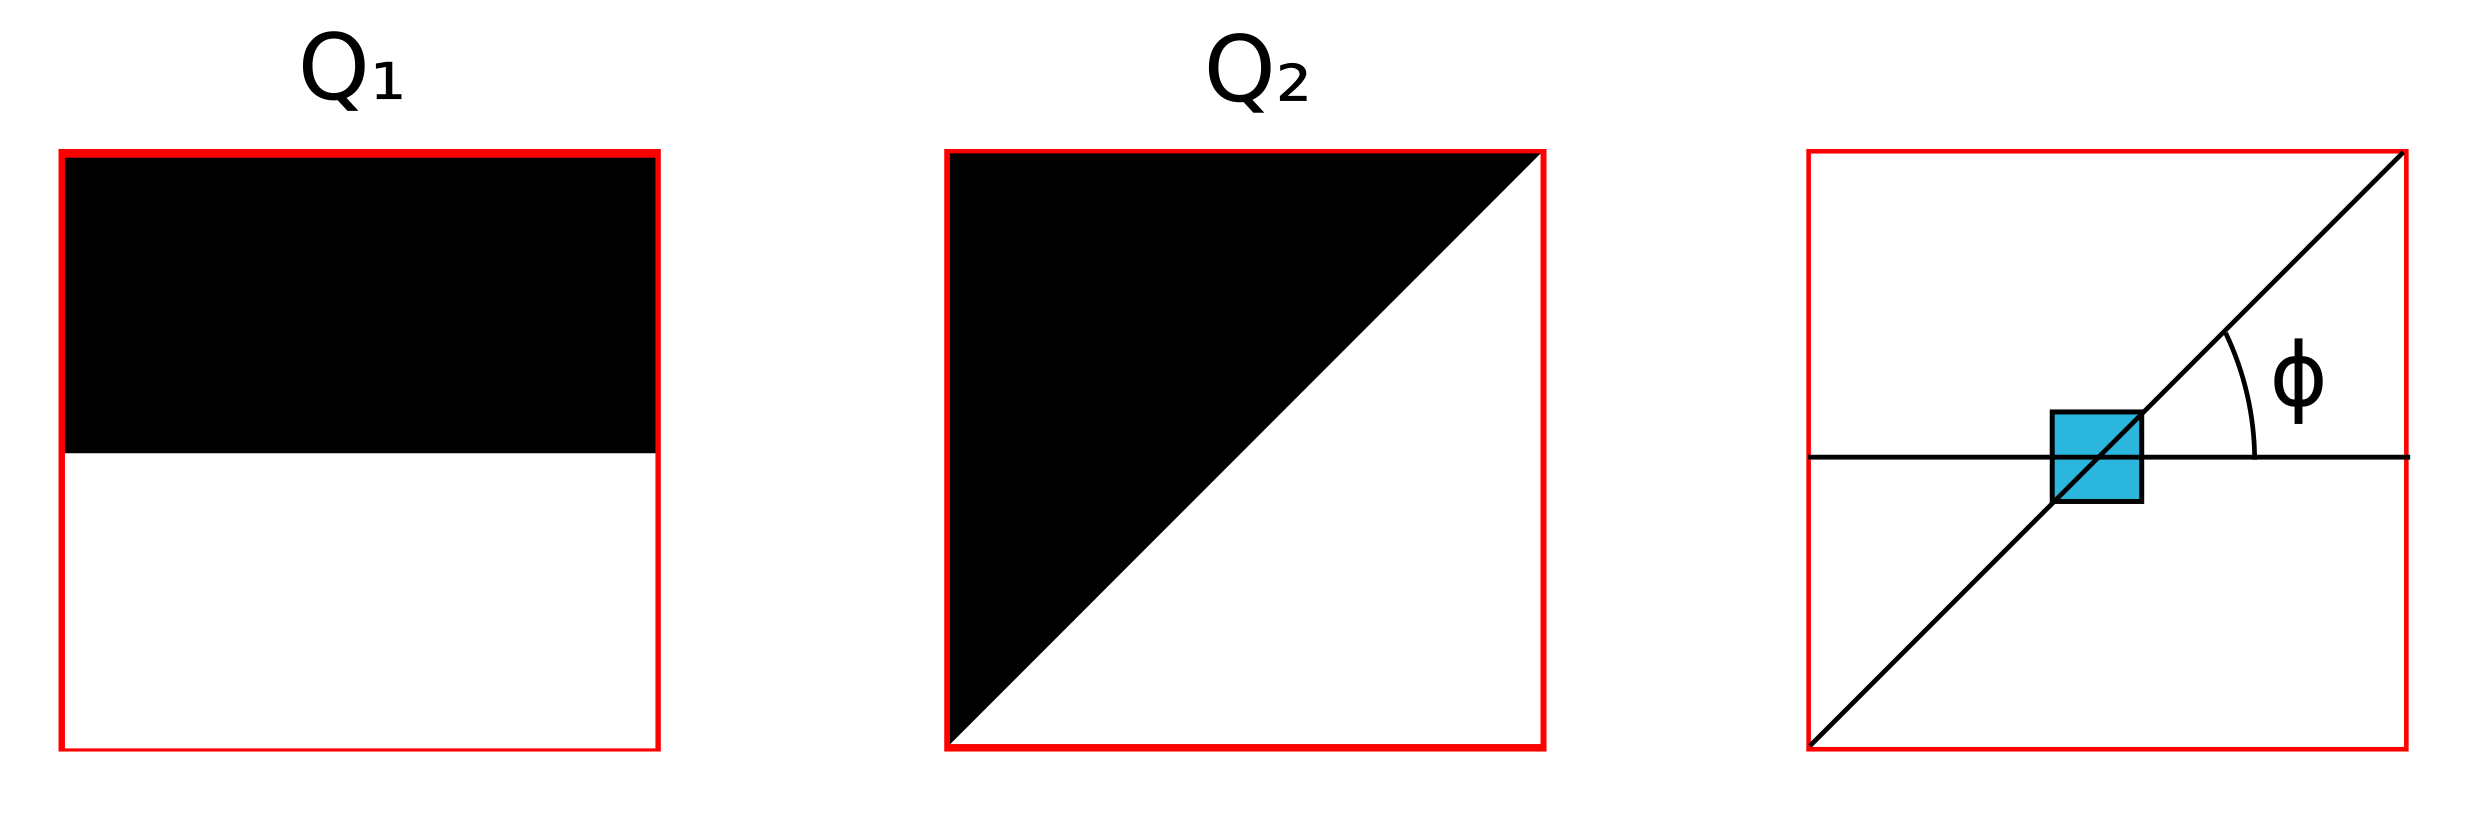
\includegraphics[width=0.8\linewidth]{images/experiment-setup.png}
  \caption[]{Left, center: images $A$ and $B$ used in the experiment for
    approximation of $1 / \sin \phi$. Right: Interfaces between phases are
    line segments which intersect each other at angle $\phi$. Shaded area is
    where $|(H*A)\cdot(H*B)|$ has non-zero values. Sum of all values in this
    area approximates $1 / \sin \phi$.}
  \label{fig:experiment-setup}
\end{figure}
Take two 2D images like the ones on \cref{fig:experiment-setup}. Boundaries
between black and white areas cross each other at the angle $\phi$. We apply an
edge detection filter to each image, multiply results element-wise and sum all
elements of the product. We want an obtained value to approximate
$1/\sin \phi$. As can be seen on \cref{fig:filter-comparison} $H'$ does this job
better than $H$. Why it's so important will be explained in the next section.
\begin{figure}
  \centering
  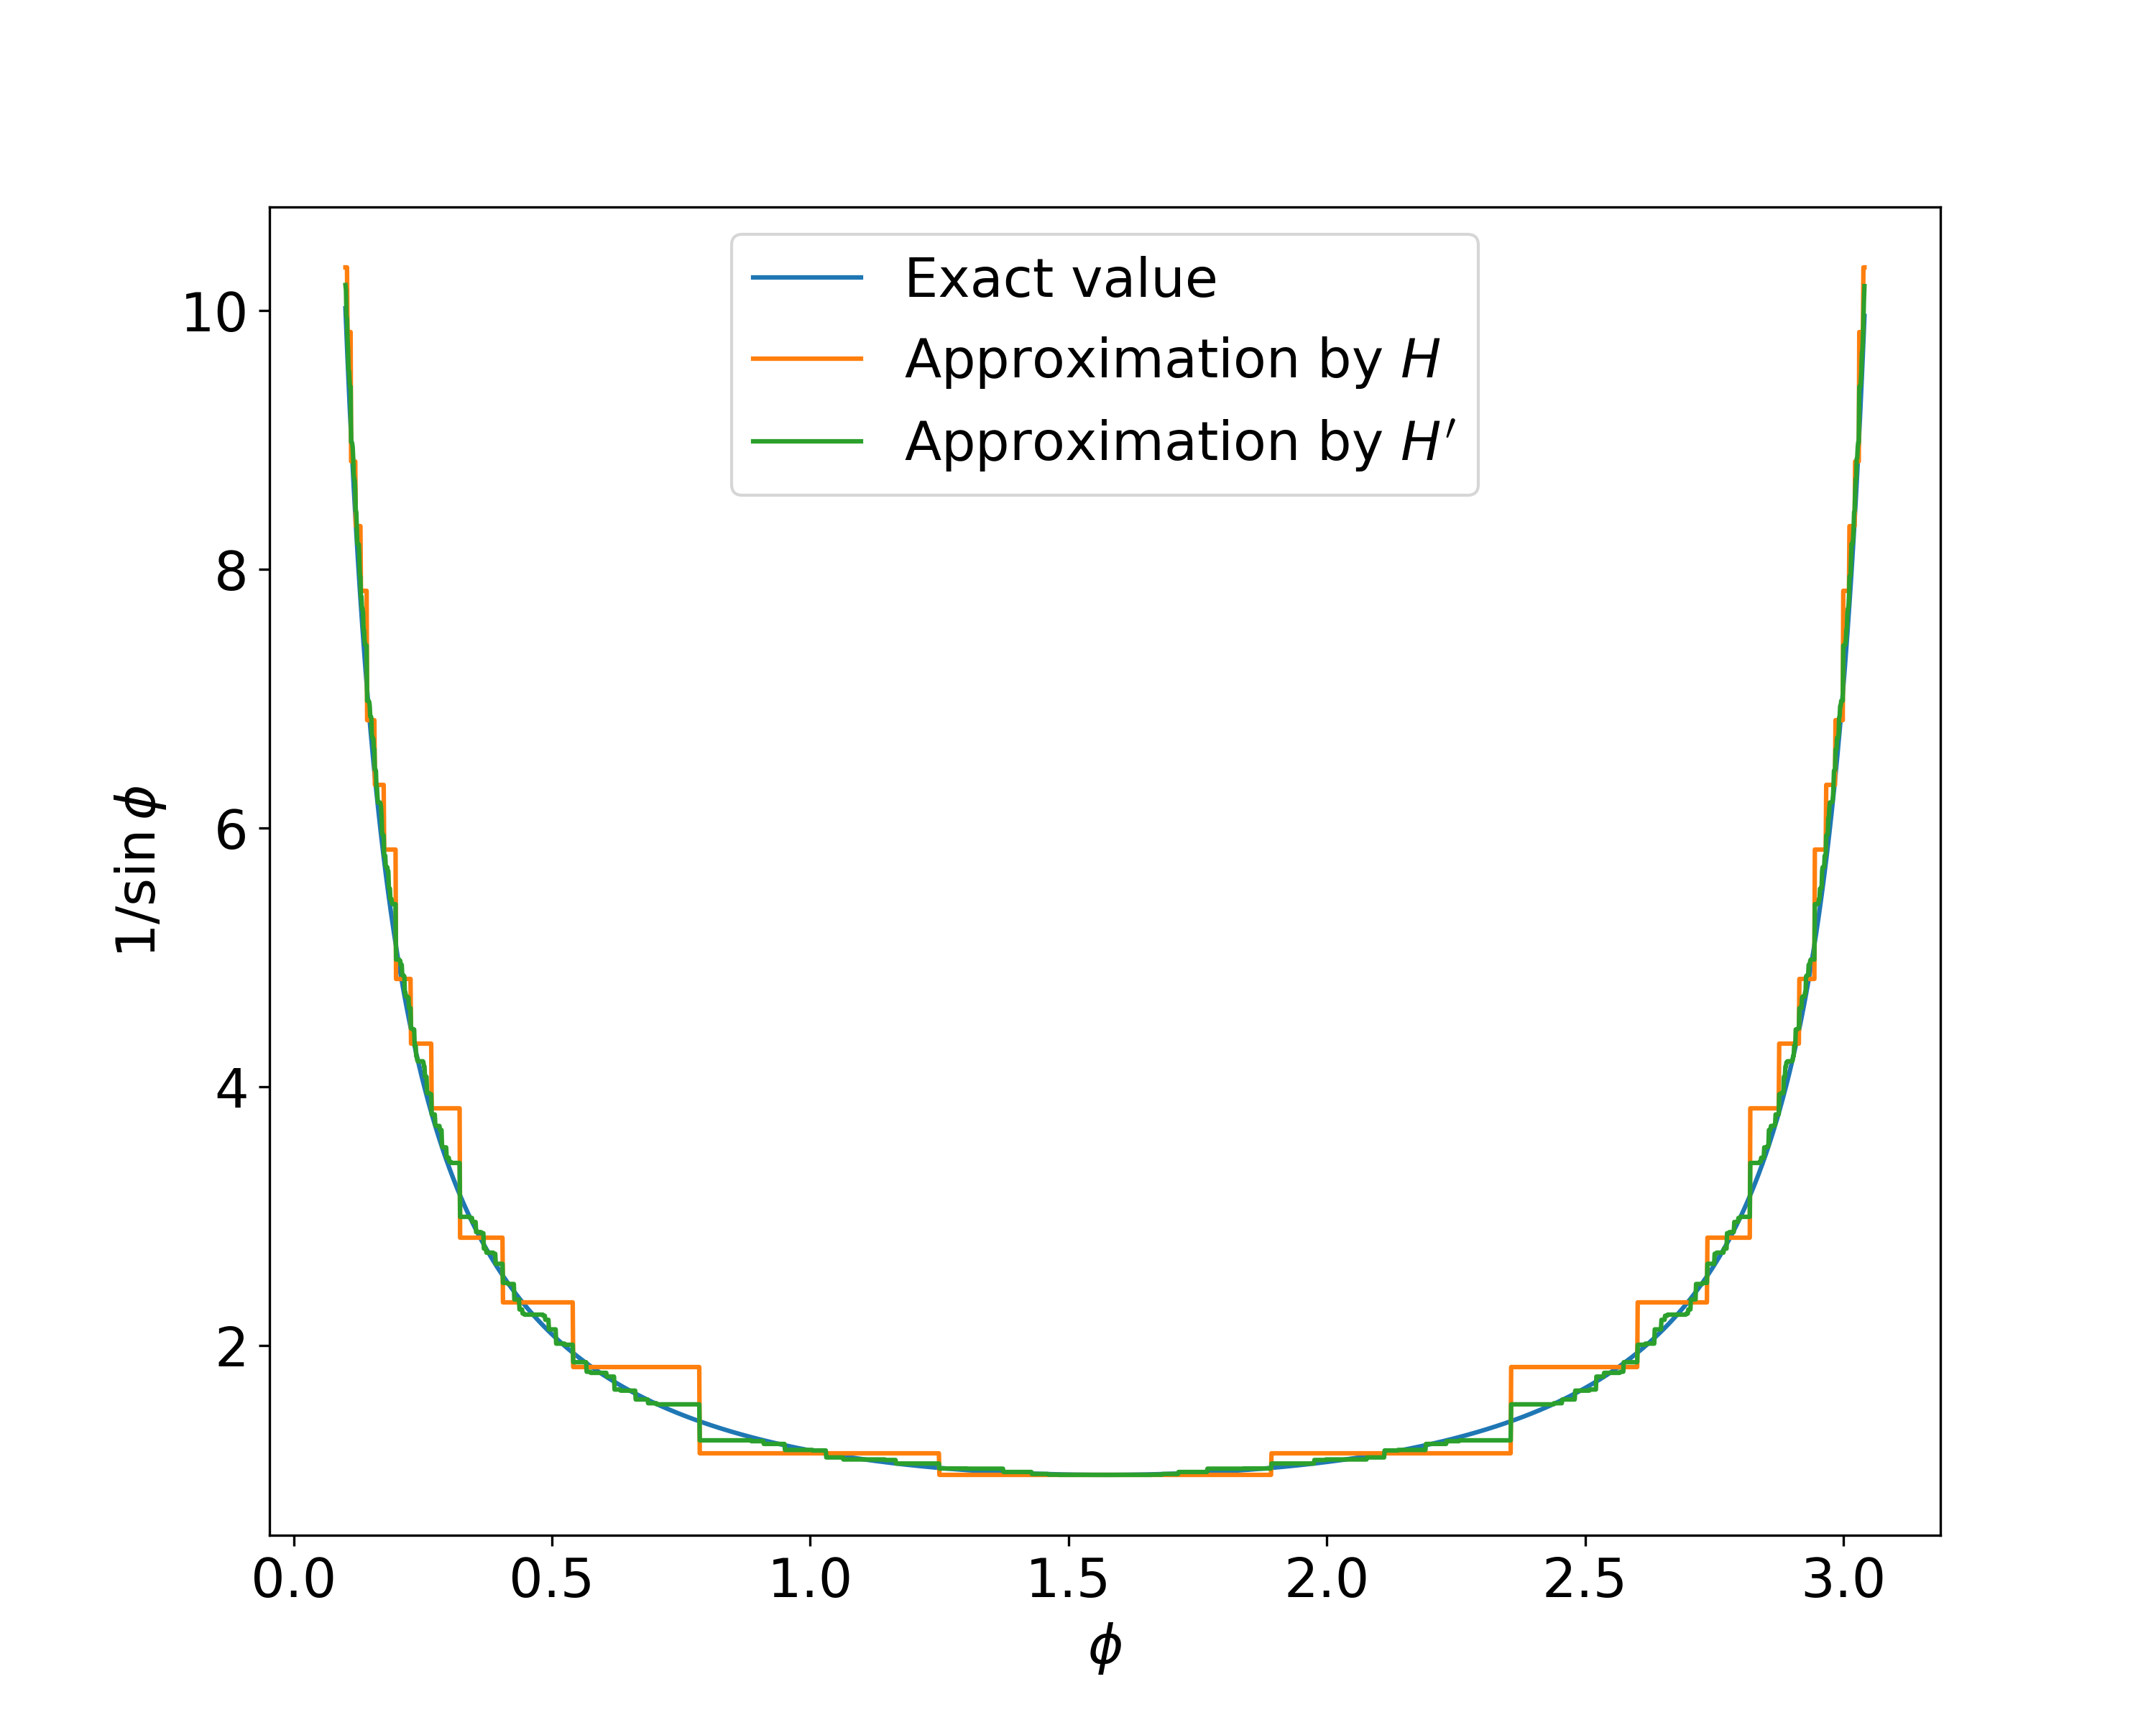
\includegraphics[width=0.8\linewidth]{images/filter-comparison.png}
  \caption[]{Estimation of $1/\sin\phi$ by filters $H$ and $H'$ in the
    experiment on \cref{fig:experiment-setup}.}
  \label{fig:filter-comparison}
\end{figure}

From now on we introduce a conventional unit of measurement ($cu$) for length.
When considering $F_{ss}$ and $F_{sv}$ functions we will work with square images
with side equal to $1\ cu$, so we can omit division by $N$ in described
algorithms and ensemble average in \cref{eq:fss} and \cref{eq:fsv} becomes a
double integral over a square $[0, 1]^2$. When considering $F_{sss}$ function we
will work with cubic images with side equal to $1\ cu$. Then we can also omit
division by $N$ and ensemble average in \cref{eq:fsss} becomes a triple integral
over a cube $[0, 1]^3$. On plots of surface functions we will omit units of
measurements in captions (e.g. we will write ``$F_{ss}$'' instead of
``$F_{ss}, cu^{-2}$''). 

\section{Computation of surface functions for sets with smooth boundary}
\label{sec:algo-precise}
In paper \textcolor{red}{our paper} we tested our algorithms for digital images
against known analytic solutions. Although we obtained acceptable results in the cases of
overlapping balls and disks, we were not sure if our algorithm performs good in
general and searched for more test cases. Here we present another test case and
develop an algorithm for calculation of $F_{ss}$ and $F_{sss}$ functions for
two- and three-dimensional sets with smooth boundary.

\subsection{Dual numbers and automatic differentiation}
\label{sec:dual}
A ring of dual numbers $D$ is a set of pairs of real numbers $(a, b)$ with two
binary operations: $+$ (addition) and $\cdot$ (multiplication) where
multiplication works according to the following law:
\begin{equation*}
  (a, b)\cdot(c, d) = (ac, ad + bc)
\end{equation*}
It's easy to see that $D$ is commutative.

It's useful to introduce an imaginary unit $\varepsilon$ and write a dual number
$(a, b)$ as $a + b\varepsilon$. As you can see from multiplication law,
$1\cdot \varepsilon = \varepsilon$ and $\varepsilon^2 = 0$, hence $D$ is not an
integral domain and division is defined only if divisor has non-zero real part:
\begin{align*}
  \frac{a+b\varepsilon}{c+d\varepsilon} &=
  \frac{(a+b\varepsilon)(c-d\varepsilon)}{(c+d\varepsilon)(c-d\varepsilon)} \\
  &= \frac{ac-ad\varepsilon+bc\varepsilon}{c^2} \\
  &= \frac{a}{c} + \frac{bc-ad}{c^2}\varepsilon
\end{align*}

Now we consider functions of dual variable $x + y\varepsilon$. Power function
$(x + y\varepsilon)^n$ where $n \in \mathbb{N}$ can be defined using binomial
formula and keeping in mind that $\varepsilon^n = 0$ if $n>1$:
\begin{equation*}
  (x + y\varepsilon)^n = \sum_{k=0}^n \binom{n}{k} x^k (y\varepsilon)^{n-k} =
  x^n + n x^{n-1} y \varepsilon
\end{equation*}
This formula can be extended to $n \in \mathbb{Q}$ as well.

Elementary functions can be extended to dual numbers using Taylor series (here
$a$ is some point at which $f$ is differentiable):
\begin{align*}
  f(x + y\varepsilon) &= f(a) + f'(a)(x + y\varepsilon) + \frac{f''(a)}{2!}(x + y\varepsilon)^2 \\
  & \qquad + \frac{f'''(a)}{3!}(x + y\varepsilon)^3 + \dots \\
  &= f(a) + f'(a)(x + y\varepsilon) + \frac{f''(a)}{2!}(x^2 + 2xy\varepsilon) \\
  & \qquad + \frac{f'''(a)}{3!}(x^3 + 3x^2y\varepsilon) + \dots \\
  &= f(a) + f'(a)x + \frac{f''(a)}{2!}x^2 + \frac{f'''(a)}{3!}x^3 + \dots \\
  & \quad y\varepsilon(f'(a) + f''(a)x + \frac{f'''(a)}{2!}x^2 + \dots) \\
  &= f(x) + yf'(x)\varepsilon
\end{align*}

Here are some basic rules for working with dual numbers (some of which we have
already described):
\begin{itemize}
\item $(a + b\varepsilon) + (c + d\varepsilon) = (a + c) + (b + d)\varepsilon$
\item $(a + b\varepsilon) (c + d\varepsilon) = ac + (ad + bc)\varepsilon$
\item $\frac{a + b\varepsilon}{c + d\varepsilon} = \frac{a}{c} + \frac{bc - ad}{c^2}$
\item $\exp(a + b\varepsilon) = \exp(a) + b\varepsilon\exp(a)$
\item $\sin(a + b\varepsilon) = \sin(a) + b\varepsilon\cos(a)$
\item $\cos(a + b\varepsilon) = \cos(a) - b\varepsilon\sin(a)$
\item $\tan(a + b\varepsilon) = \tan(a) - \frac{b}{cos^2(a)}\varepsilon$
\end{itemize}

As you can see, dual numbers are connected with differentiation. Using a dual
argument $a + \varepsilon$ we can compute a value of a function at point $x = a$
and its derivative at that point:
$f(a + \varepsilon) = f(a) + f'(a)\varepsilon$. Also we can compute a partial
derivative of a multivariate function. For example:
\begin{equation}
  \begin{aligned}
    \frac{\partial}{\partial x} f(x, y) \vert_{x = a, y = b} &= f(a + \varepsilon,
    b) \\
    \frac{\partial}{\partial y} f(x, y) \vert_{x = a, y = b} &= f(a, b +
    \varepsilon)
  \end{aligned}
  \label{eq:autonormals}
\end{equation}
The last equation will be useful for computation of normals to the interface in
next sections.

\subsection{Surface-surface function for two-dimensional sets with smooth boundary}
\label{sec:fss-2d}
\begin{figure}
  \centering
  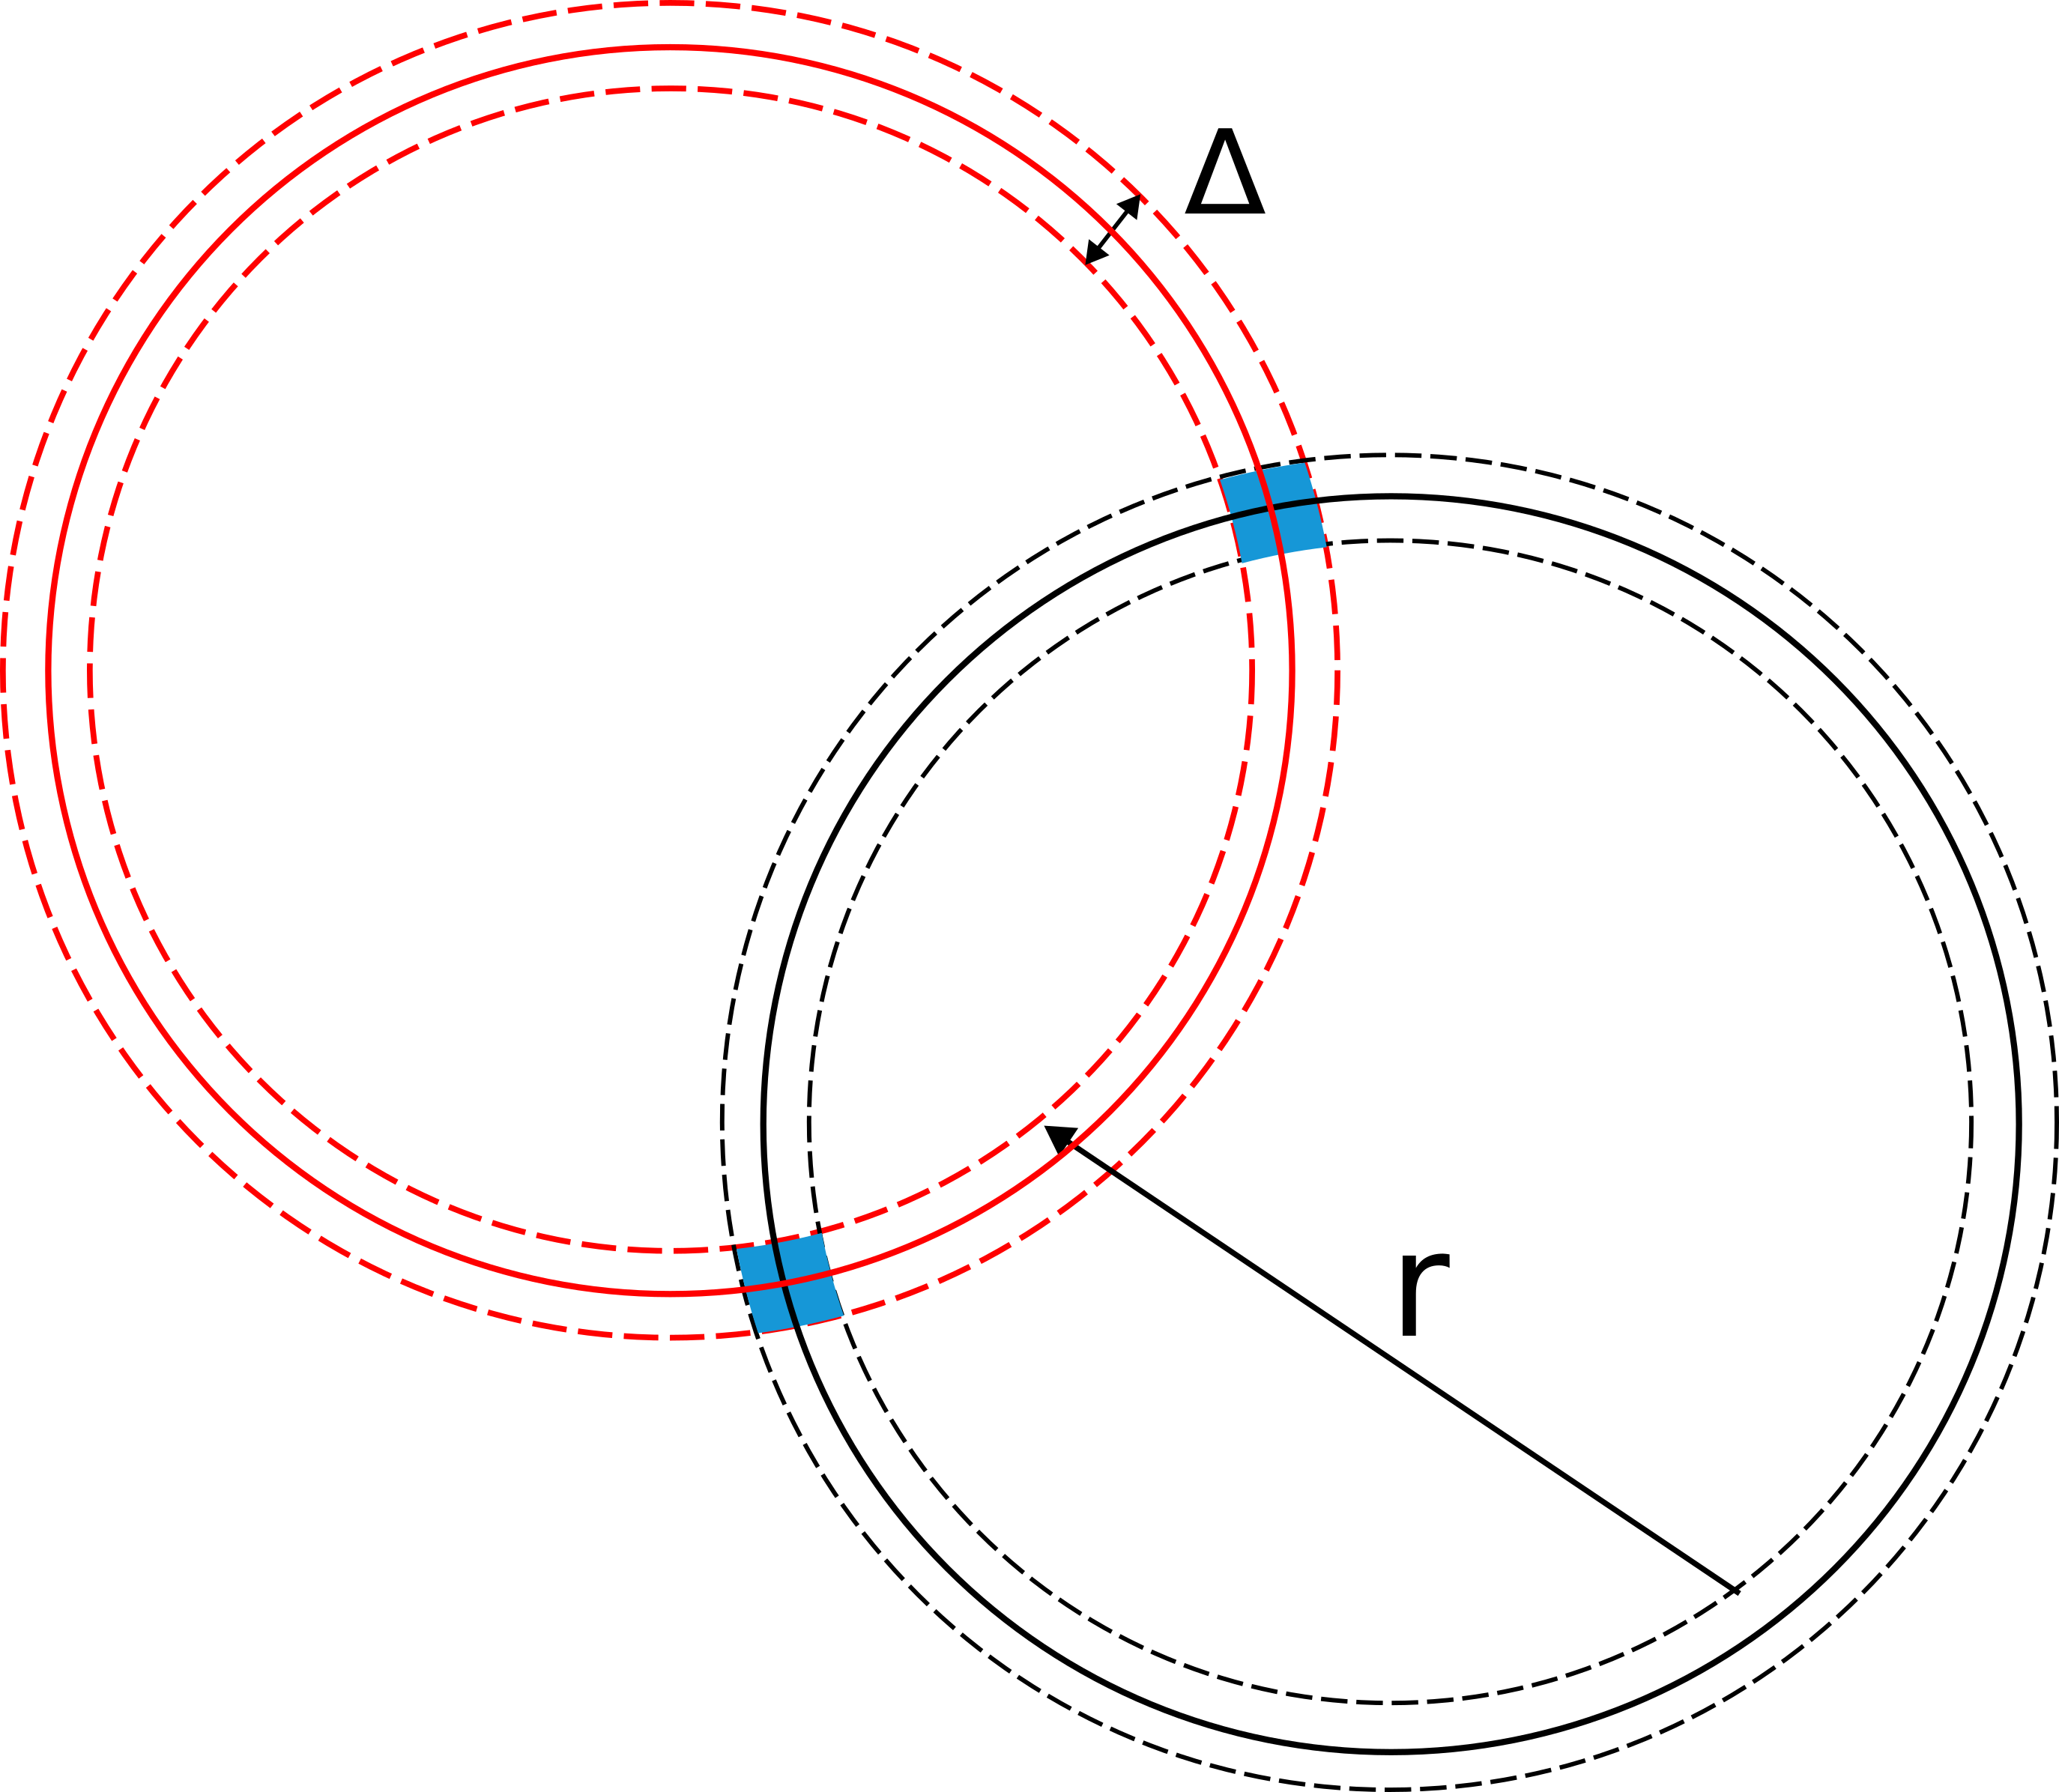
\includegraphics[width=0.8\linewidth]{images/Fss.png}
  \caption[]{Illustration of how $F_{ss}(\bm{r})$ is calculated. The interface
    between solid and void phases is a solid black curve. This interface
    translated by the vector $\bm{r}$ is show as a red solid curve. Support of
    $f_\Gamma(\bm{x}; \Delta)$ is a dashed ring. Shaded regions contribute to
    the surface-surface function.}
  \label{fig:Fss-explained}
\end{figure}
Let $S$ be some set in $\mathbb{R}^2$ which has a smooth boundary $\Gamma$ in
the sense that the boundary has a tangent line almost everywhere. Now we
introduce a function $f_\Gamma(\bm{x}; \Delta)$:
\begin{equation}
  f_\Gamma(\bm{x}; \Delta) = \left\{
  \begin{array}{ll}
    1/\Delta & \quad \rho(\bm{x}, \Gamma) < \Delta \\
    0 & \quad \text{otherwise}
  \end{array}
  \right. \label{eq:delta-sequence}
\end{equation}
Here $\rho(\bm{x}, \Gamma)$ means a closest distance from point $\bm{x}$ to the
boundary $\Gamma$.

\begin{figure}
  \centering
  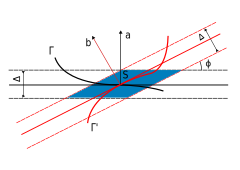
\includegraphics[width=0.8\linewidth]{images/fss-zoomed.png}
  \caption[]{Zoomed image of intersection between the interface $\Gamma$ and its
    translated version $\Gamma'$. $\phi$ is an angle between tangent lines to
    the interfaces. Surface of dashed area is
    $\frac{\Delta^2}{\sin \phi}$. Vectors $\bm{a}$ and $\bm{b}$ are unit vectors
    parallel to normals to $\Gamma$ and $\Gamma'$ respectively in the point of
    their intersection.}
  \label{fig:fss-zoomed}
\end{figure}
Now define a functional sequence $F_{ss}(\bm{r}; \Delta)$:
\begin{align*}
  F_{ss}(\bm{r}; \Delta) &= \int\int f_\Gamma(\bm{x}; \Delta) f_\Gamma(\bm{x}
  + \bm{r}; \Delta) dx dy \\
  &= \sum_{k=1}^N S_k/\Delta^2
\end{align*}
Here $N$ is a number of intersections of $\Gamma$ with itself translated by a
vector $\bm{r}$ and $S_k$ is a surface of each such intersection (see
\cref{fig:Fss-explained}).
When $\Delta$ tends to zero, the boundary at the point of intersection can
be replaced with a tangent line at the point of intersection
(\cref{fig:fss-zoomed}). We get an expression for a surface of
intersection: $S_k = \frac{\Delta^2}{\sin \phi_k}$ where $\phi_k$ is an
acute angle between tangent lines. Hence, we get the following equation:
\begin{equation}
  F_{ss}(\bm{r}) = \lim_{\Delta \to 0} F_{ss}(\bm{r}; \Delta) =
  \sum_{k=1}^N \frac{1}{\sin \phi_k} \label{eq:fss-2d-sin}
\end{equation}
It's easy to show that
$\lim_{\Delta \to 0} f_\Gamma(\bm{x}; \Delta) = |\nabla \chi_A(\bm{x})|$
and therefore \cref{eq:fss-2d-sin} and \cref{eq:fss} define the same
function. This equation for $F_{ss}$ also explains why edge detection filters
need to approximate $1/\sin \phi_k$ and why the filter \cref{eq:filter-7x7} is
better than \cref{eq:filter-3x3}.

A less illustrative but more practical way to calculate an expression
$\frac{S_k}{\Delta}$ is the following. Take two vectors $\bm{a}$ and $\bm{b}$
parallel to normals to $\Gamma$ and $\Gamma'$ in $k$-th point of their
intersection such as $|a| = |b| = 1$. If $F_{ss}$ is defined at the point of
consideration then $\bm{a} \ne \pm \bm{b}$. The pair $(\bm{a}, \bm{b})$ may
serve as a basis with the following transformation from the basis
$(1,0), (0,1)$:
\begin{align*}
  x' &= f(x, y) = a_x x + a_y y \\
  y' &= g(x, y) = b_x x + b_y y
\end{align*}
where $\bm{a} = (a_x, a_y)$, $\bm{b} = (b_x, b_y)$. Jacobian determinant for
this transformation is
\begin{equation*}
  J = \left|
  \begin{array}{cc}
    \frac{\partial f}{\partial x} & \frac{\partial f}{\partial y} \\
    \frac{\partial g}{\partial x} & \frac{\partial g}{\partial y} \\
  \end{array}
  \right| =
  \left|
  \begin{array}{cc}
    a_x & a_y \\
    b_x & b_y
  \end{array}
  \right| = a_x b_y - a_y b_x
\end{equation*}

We can rewritte \cref{eq:fss-2d-sin} using $J$ as follows:
\begin{equation}
  F_{ss}(\bm{r}) = \sum_{k=1}^N \frac{1}{|J_k|} \label{eq:fss-2d}
\end{equation}
where $J_k$ is Jacobian determinant computed at $k$-th point of
intersection. This form proves to be much more useful than the version which
contains the angle $\phi$.

Now we get to practical algorithm for computation of $F_{ss}$ for sets with a
smooth boundary. Suppose a set $S$ is defined as
$S = \left\{ (x, y) \ | \quad f(x, y) \le T \right\}$ where $f(x, y)$ is some
function differentiable at points where $f(x, y) = T$ and $T$ is some
threshold. Let's calculate surface-surface function for this set at a point
$\bm{r} = (r_x, r_y)$. We find all intersections between a boundary $\Gamma$ and
its translated version by solving a system of equations
\begin{equation*}
  \left\{
  \begin{array}{l}
    f(x, y) = T \\
    f(x-r_x, y-r_y) = T
  \end{array}
  \right.
\end{equation*}
which can be replaced by one equation
\begin{equation}
  (f(x, y) - T)^2 + (f(x-r_x, y-r_y) - T)^2 = 0 \label{eq:inter}
\end{equation}
We denote a set of solutions of this equation as $X$. For every $\bm{x}_i \in X$
we find normals to the boundary and the boundary translated by a vector
$\bm{r}$. These normals can be found using automatic differentiation and dual
numbers described in \cref{sec:dual}. Then we normalize these normals (i.e. make
their length equal to $1$) and use \cref{eq:fss-2d} to calculate $F_{ss}$.

Summarizing, the algorithm of calculating $F_{ss}(\bm{r})$ is the following:
\begin{enumerate}
\item Find $X$ which is a set of soulutions of \cref{eq:inter}.
\item For all points in $X$ find normals to the boundaries using
  \cref{eq:autonormals} and normalize them.
\item Calculate $F_{ss}(\bm{r})$ using \cref{eq:fss-2d}.
\end{enumerate}

The set $X$ can be found by firstly evaluating $f(x, y)$ in some regular grid
searching for all points $(x_i, y_i)$ for which $|f(x_i, y_i) - T| < \epsilon$
and $|f(x_i - r_x, y_i - r_y) - T| < \epsilon$ for some positive $\epsilon$
and then using these points as starting points for some algorithm based on
gradient descent like ADAM to solve \cref{eq:inter}.

\subsection{Surface-surface-surface function for three-dimensional sets with
  smooth boundary}
\label{sec:fsss-3d}
Results of this section are made by analogy with \cref{sec:fss-2d}. Again, let
$S$ be some set in $\mathbb{R}^3$ which has a smooth boundary, i.e. has a
tangent plane at almost every point of its boundary. Using the function
\cref{eq:delta-sequence} we define a functional sequence
$F_{sss}(\bm{r_1}, \bm{r_2}; \Delta)$:
\begin{align*}
  F_{sss}(\bm{r_1}, \bm{r_2}; \Delta) &= \int\int\int dx dy dz \times \\
  &\qquad \times f_\Gamma(\bm{x}; \Delta) f_\Gamma(\bm{x} + \bm{r_1}; \Delta)
  f_\Gamma(\bm{x} + \bm{r_2}; \Delta) \\
  &= \sum_{k=1}^N V_k/\Delta^3
\end{align*}
$V_k$ is a volume of parallelepiped where all three multiplicands under integral
are non-zero. $N$ is a number of these parallelepipeds, i.e. number of points
where all three boundaries (one ``original'' boundary and two translated
versions) have an intersection. With $\Delta$ going to zero we get a convergence
to $F_{sss}$:
\begin{equation*}
  \lim_{\Delta \to 0} F_{sss}(\bm{r_1}, \bm{r_2}; \Delta) = F_{sss}(\bm{r_1},
  \bm{r_2})
\end{equation*}

Let $\bm{a}$, $\bm{b}$ and $\bm{c}$ be normalized normals to each boundary in
the point of intersection. The corresponding $V_k$ is finite if and only if
$\bm{a} \ne \pm \bm{b} \ne \pm \bm{c}$. In this case we can use a triplet
$(\bm{a}, \bm{b}, \bm{c})$ as basis for $\mathbb{R}^3$ with the following
transformation from the basis $(1,0,0), (0,1,0), (0, 0, 1)$:
\begin{align*}
  x' &= f(x, y) = a_x x + a_y y + a_z z \\
  y' &= g(x, y) = b_x x + b_y y + b_z z \\
  z' &= h(x, y) = c_x x + c_y y + c_z z \\
\end{align*}
Jacobian determinant for this transformation is
\begin{equation*}
  J = \left|
  \begin{array}{ccc}
    a_x & a_y & a_z \\
    b_x & b_y & b_z \\
    c_x & c_y & c_z \\
  \end{array}
  \right|
\end{equation*}
and the expression for $F_{sss}$ becomes
\begin{equation}
  F_{sss}(\bm{r_1}, \bm{r_2}) = \sum_{k=1}^N \frac{1}{|J_k|} \label{eq:fsss-3d}
\end{equation}
where $J_k$ is Jacobian determinant computed at $k$-th point of
intersection.

\section{Results}
\label{sec:results}
In this section we will provide few examples of sets for which the developed
precise algorithm is applicable and compare the surface-surface function
calculated with the algorithm for digital images (\cref{sec:algo}) with results
of the new algorithm. We will use the filter $H$ (\ref{eq:filter-3x3}) for edge
detection along with a new filter $H'$ (\ref{eq:filter-7x7}) proposed in this
paper.

\subsection{A square and a cube}
Define a function $f(\bm{x}) = \max\limits_i |x_i|$. A set $f(\bm{x}) \le T$
where $\bm{x} \in \mathbb{R}^2$ is a square with side $2T$. The function $f$ is
differentiable at all points where $f(\bm{x}) = T$ with exception of points
$(-T, -T)$, $(-T, T)$, $(T, -T)$ and $(T, T)$. The surface-surface correlation
function for a square is equal to:
\begin{equation*}
  F_{ss}(\bm{r}) = \left\{
  \begin{array}{ll}
    2 & \quad f(\bm{r}) < 2T \ \text{and}\ r_i \ne 0, \forall i \in \overline{1,2} \\
    0 & \quad f(\bm{r}) > 2T \\
    \text{undefined} & \quad \text{otherwise}
  \end{array}
  \right.
\end{equation*}
A graphical diagram depicting this case is shown on \cref{fig:fss-square}. In
this case the algorithm described in \cref{sec:algo} gives a correct result in
any point which is few pixels away from where $F_{ss}$ is undefined.
\begin{figure}
  \centering
  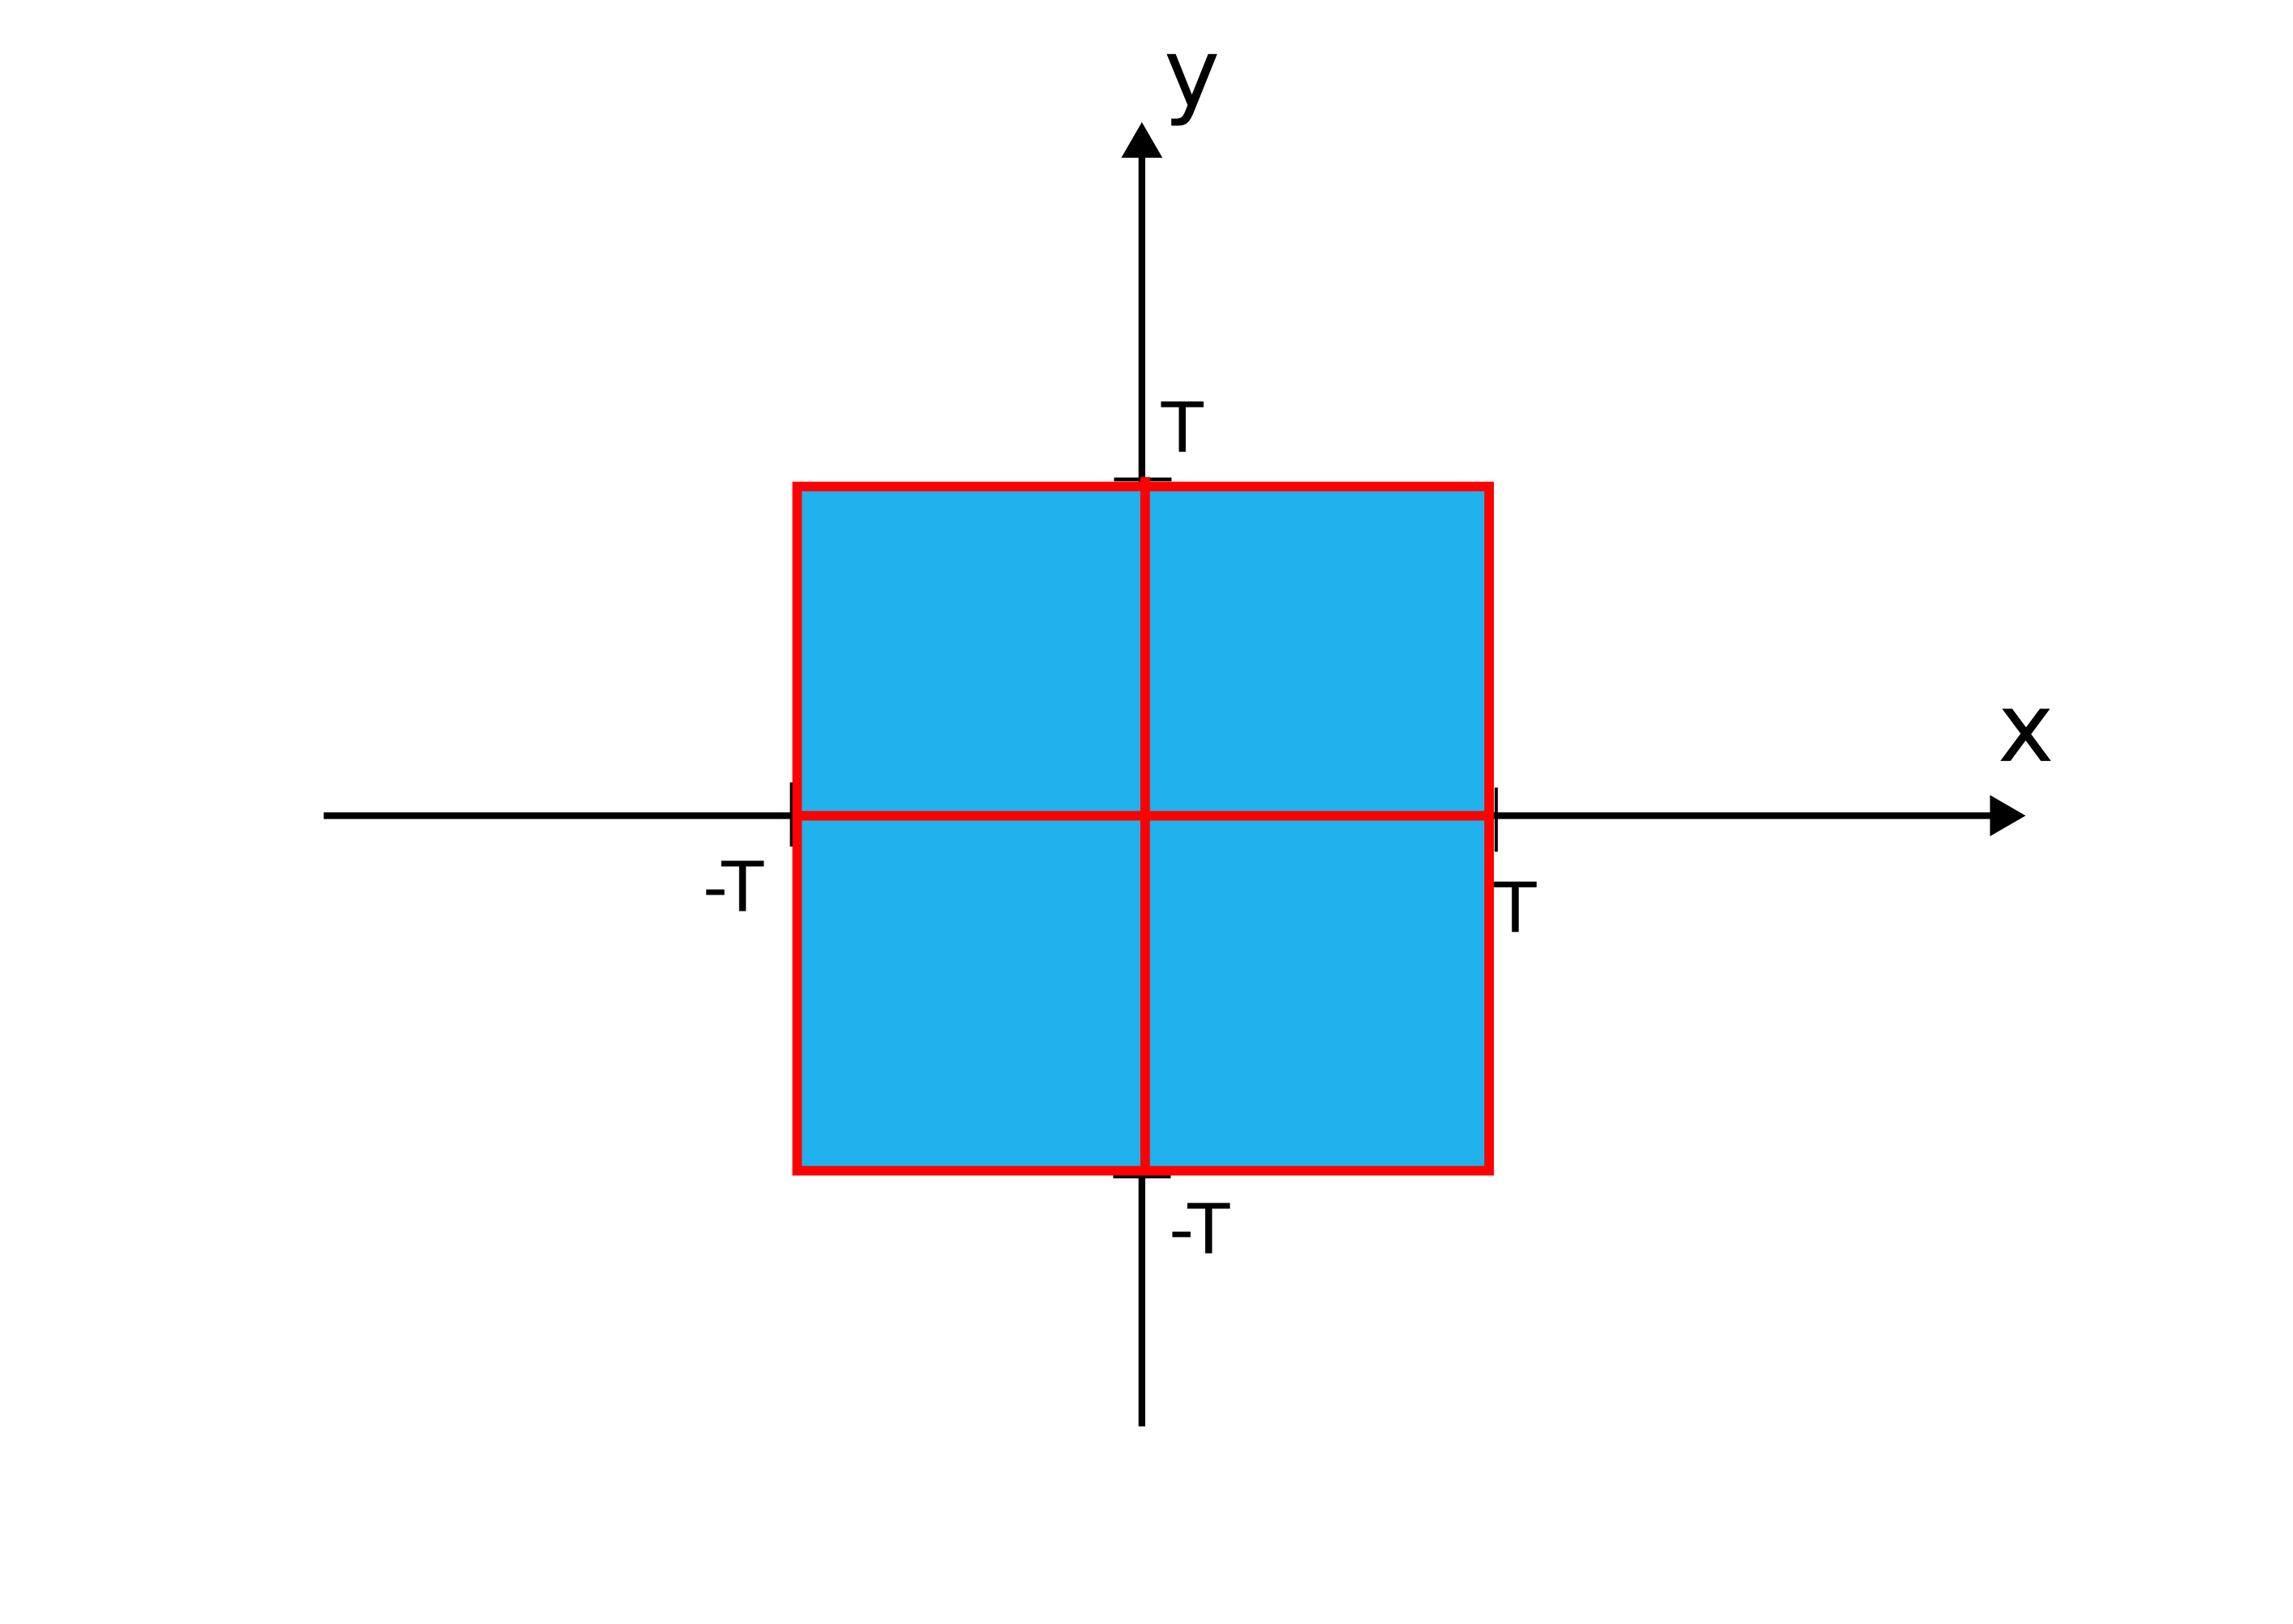
\includegraphics[width=0.45\linewidth]{images/fss-square.png}
  \hfill
  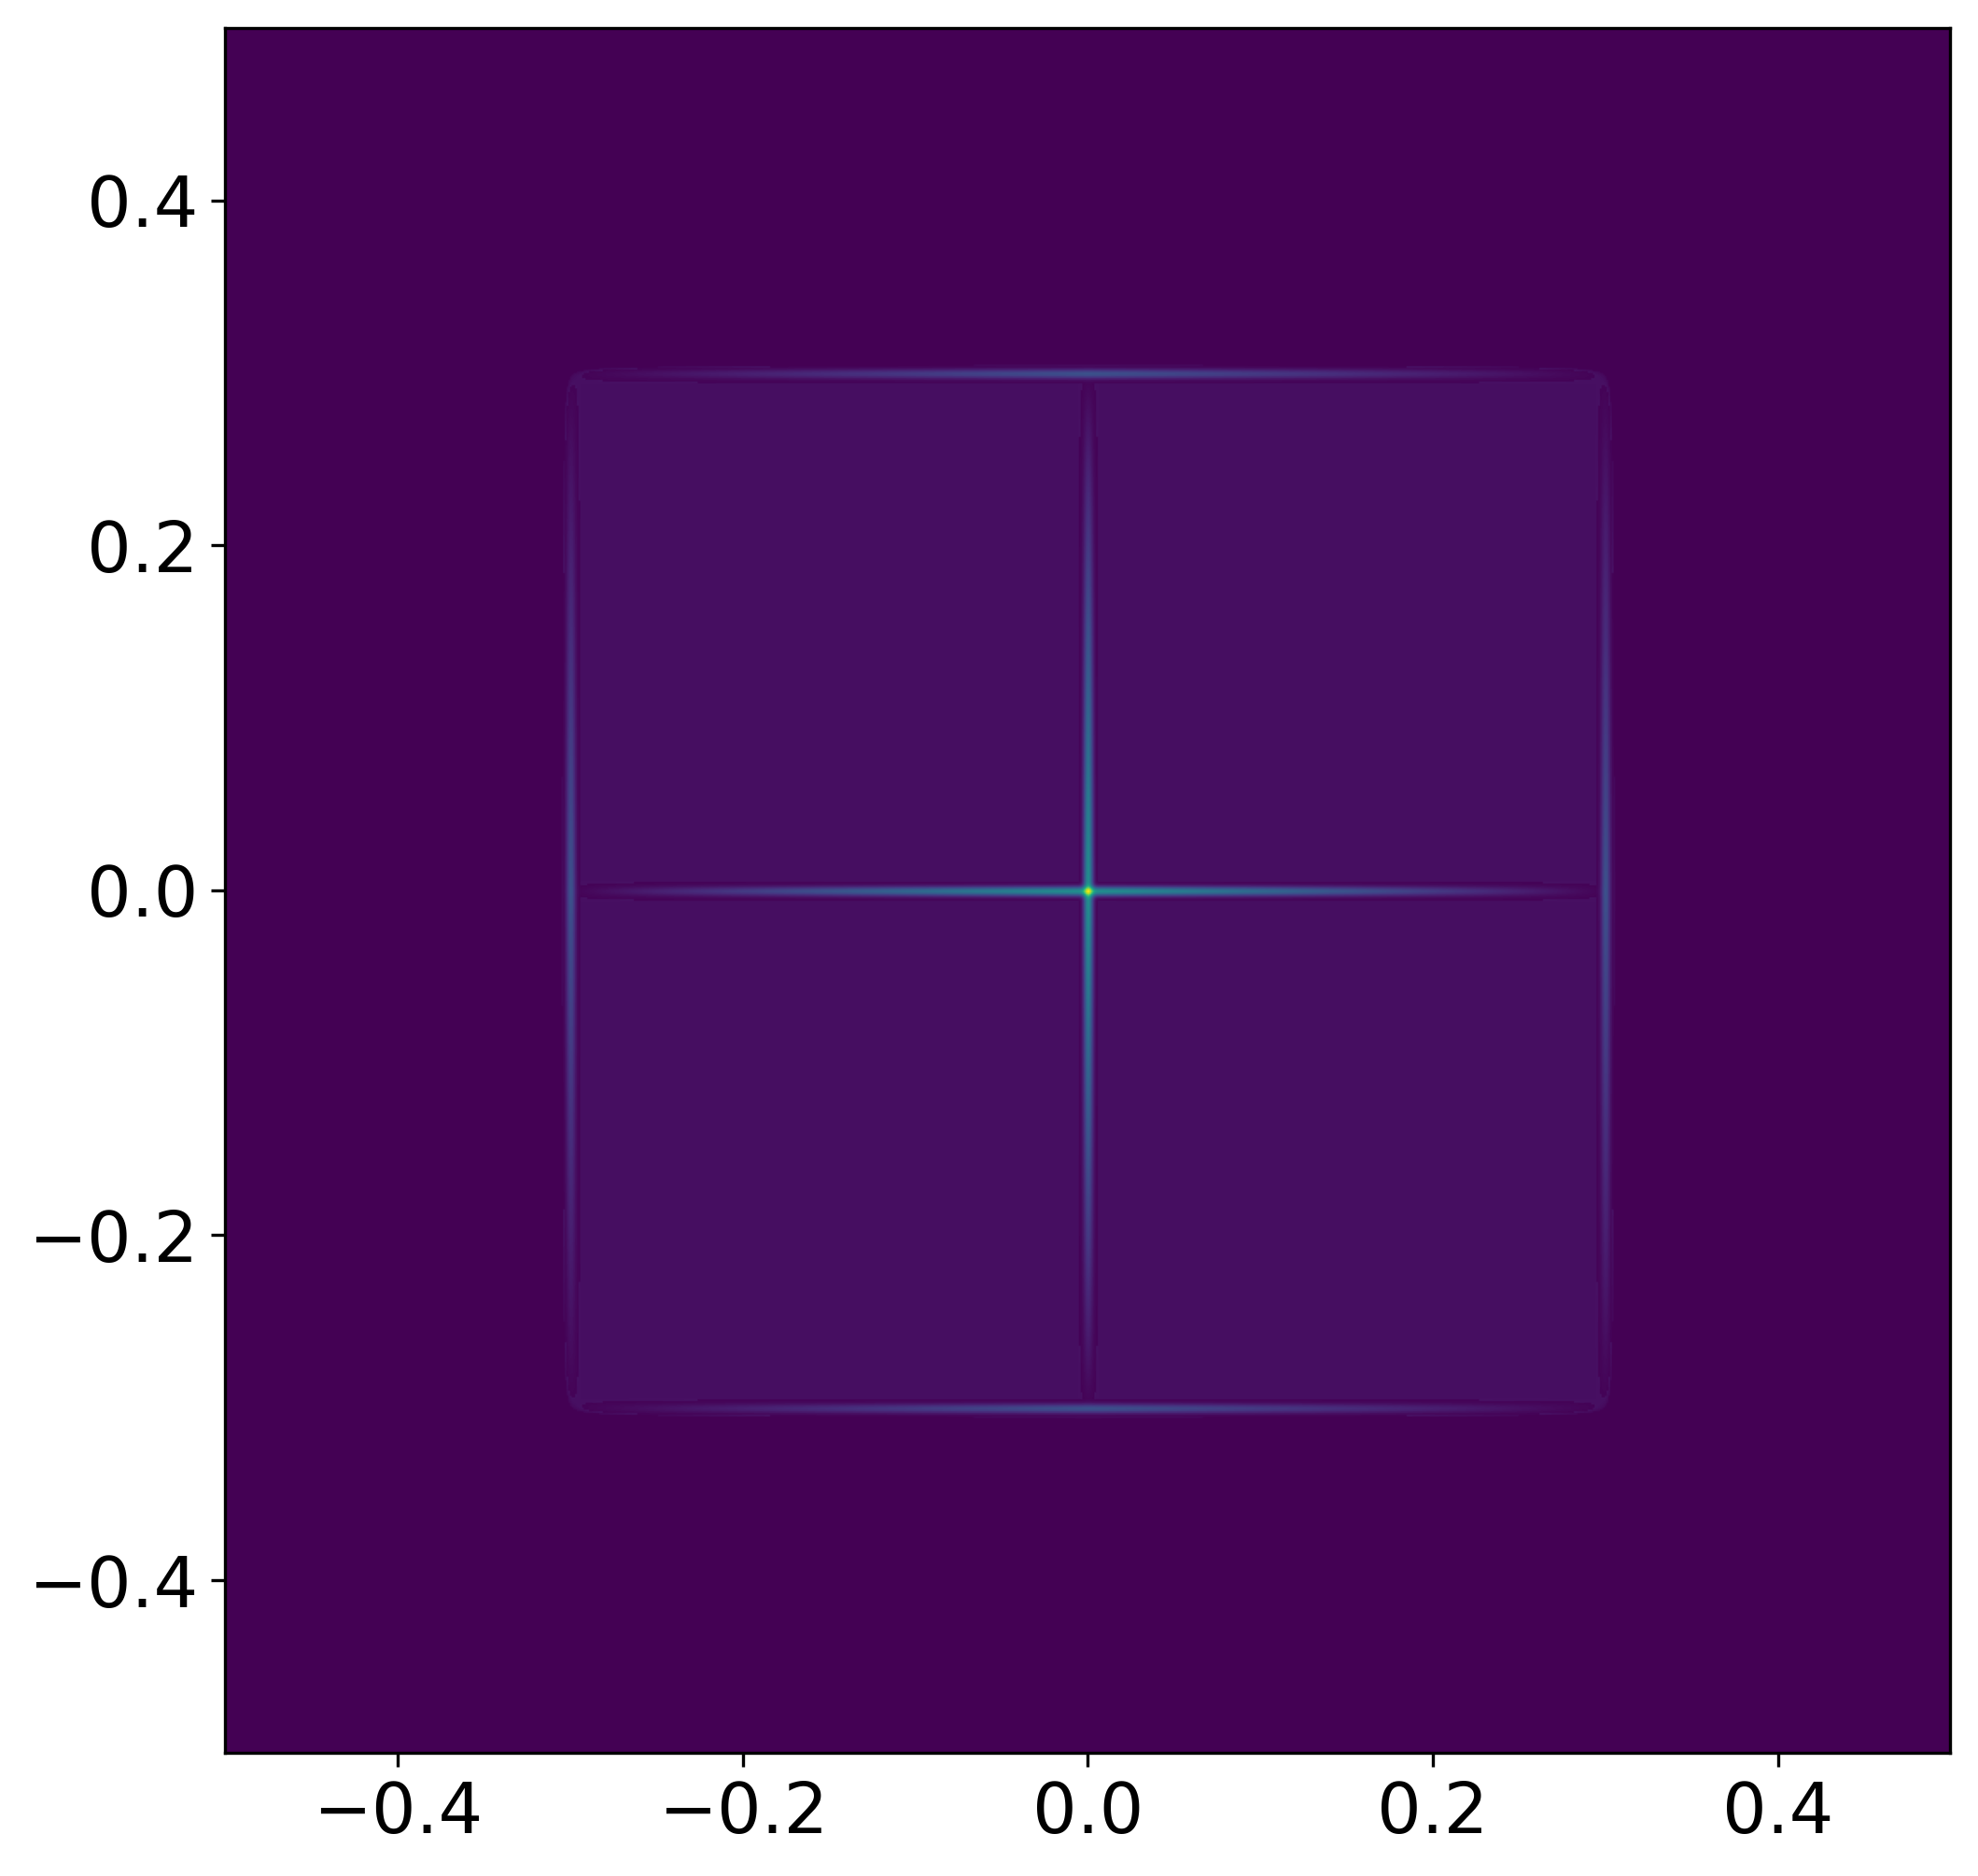
\includegraphics[width=0.45\linewidth]{images/fss-square-julia.png}
  \caption[]{$F_{ss}$ function for a square with side $T = 0.3$. On the left:
    Theoretical results. The function is undefined along red segments. Its value
    is $2$ inside a shaded area and $0$ outside. On the right: Calculation with
    the algorithm described in \cref{sec:algo}.}
  \label{fig:fss-square}
\end{figure}

A set $f(\bm{x}) \le T$ where $\bm{x} \in \mathbb{R}^3$ is a cube with the same
side $2T$.
The surface-surface-surface correlation function for this cube is equal to:
\begin{equation*}
  F_{sss}(\bm{r}) = \left\{
  \begin{array}{ll}
    2 & \quad f(\bm{r}) < 2T \ \text{and}\ r_i \ne 0, \forall i \in \overline{1,3} \\
    0 & \quad f(\bm{r}) > 2T \\
    \text{undefined} & \quad \text{otherwise}
  \end{array}
  \right.
\end{equation*}
This case is also handled good by the algorithm described in
\cref{sec:algo}. Plot of $F_{sss}$ for this case is trivial and not shown here.

\subsection{A disk and a ball}
Define $f(\bm{x}) = \sum_i x_i^2$. If $\bm{x} \in \mathbb{R}^2$ when an
inequation $f(\bm{x}) \le R^2$ defines a disk of radius $R$ with the center at
the origin. In this case $F_{ss}$ depends only on distance $r$ from the origin:
\begin{equation*}
  F_{ss}(r) = \left\{
  \begin{array}{ll}
    \frac{4R^2}{r\sqrt{4R^2-r^2}} & \quad r < 2R \\
    0 & \quad \text{otherwise}
  \end{array}
  \right.
\end{equation*}
A comparison of the algorithm described in \cref{sec:algo} applied to images
with different resolution with a theory is shown on \cref{fig:fss-disk}.
\begin{figure*}[!hpt]
  \centering
  \subfigure[$3\times 3$ kernel $H$]{
    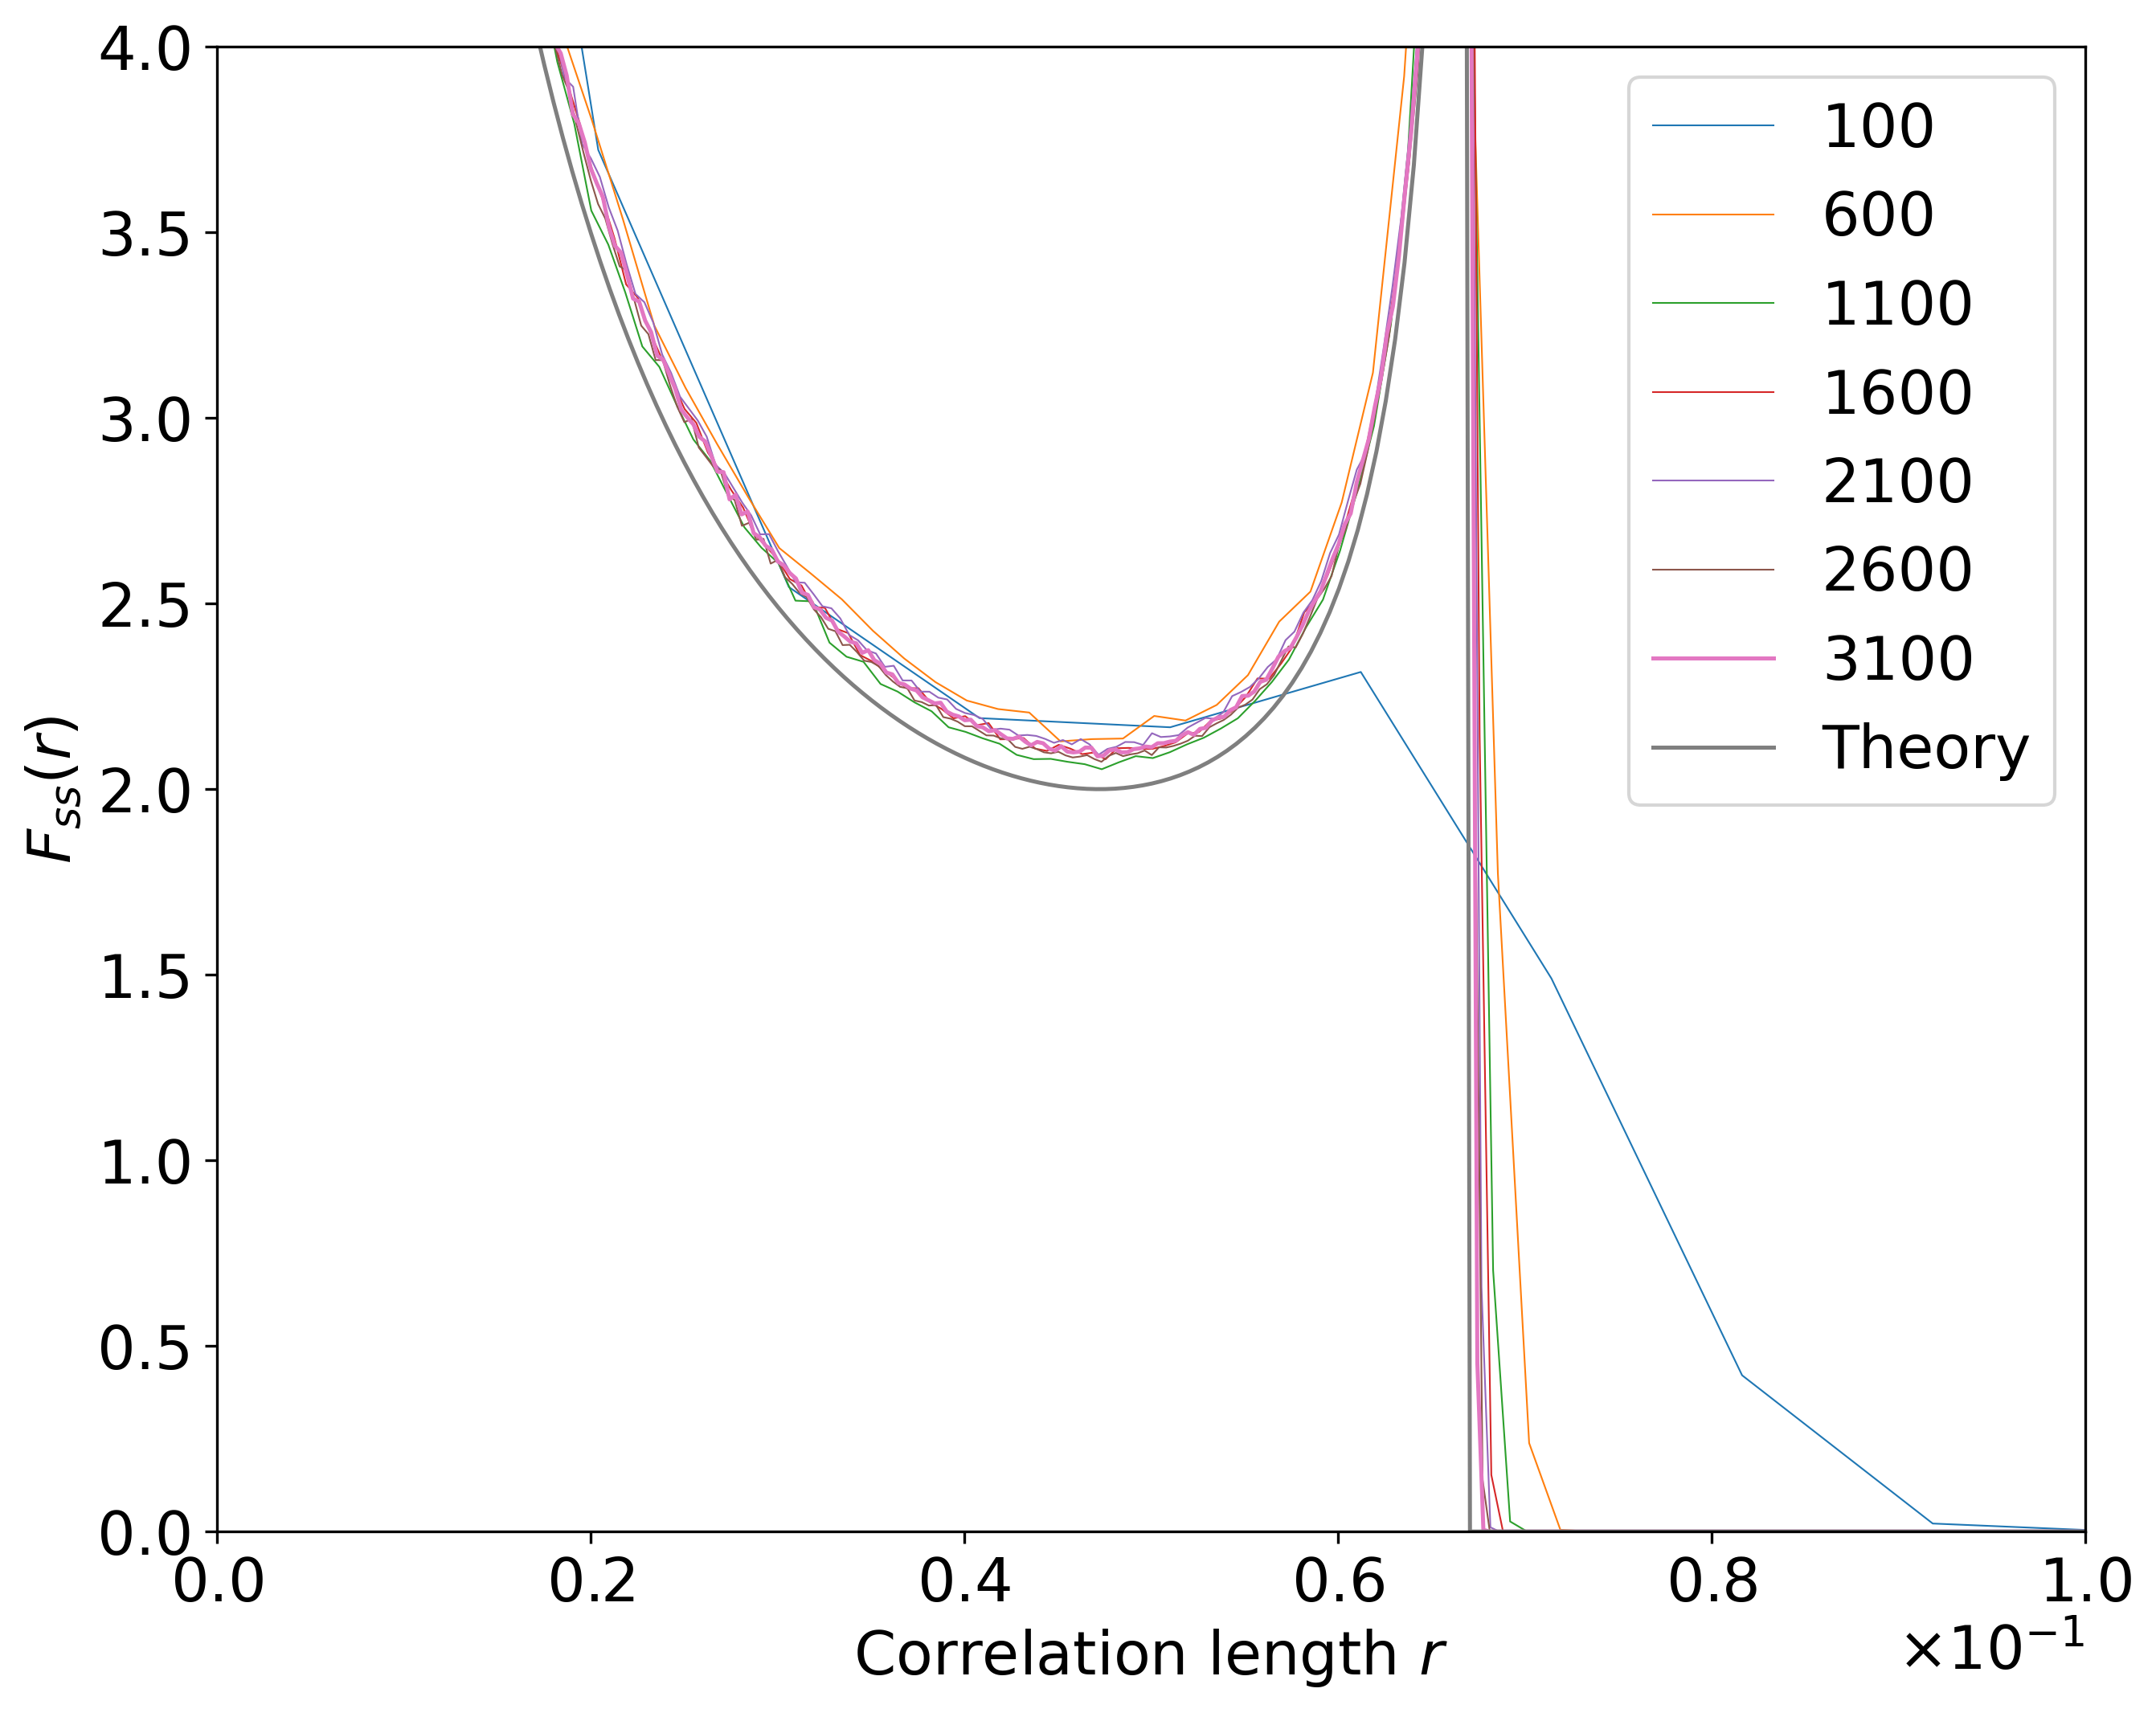
\includegraphics[width=0.45\linewidth]{images/fss-disk-3x3.png}
    \label{fig:fss-disk-3x3}}
  \hfill
  \subfigure[$5\times 5$ kernel $H'$]{
    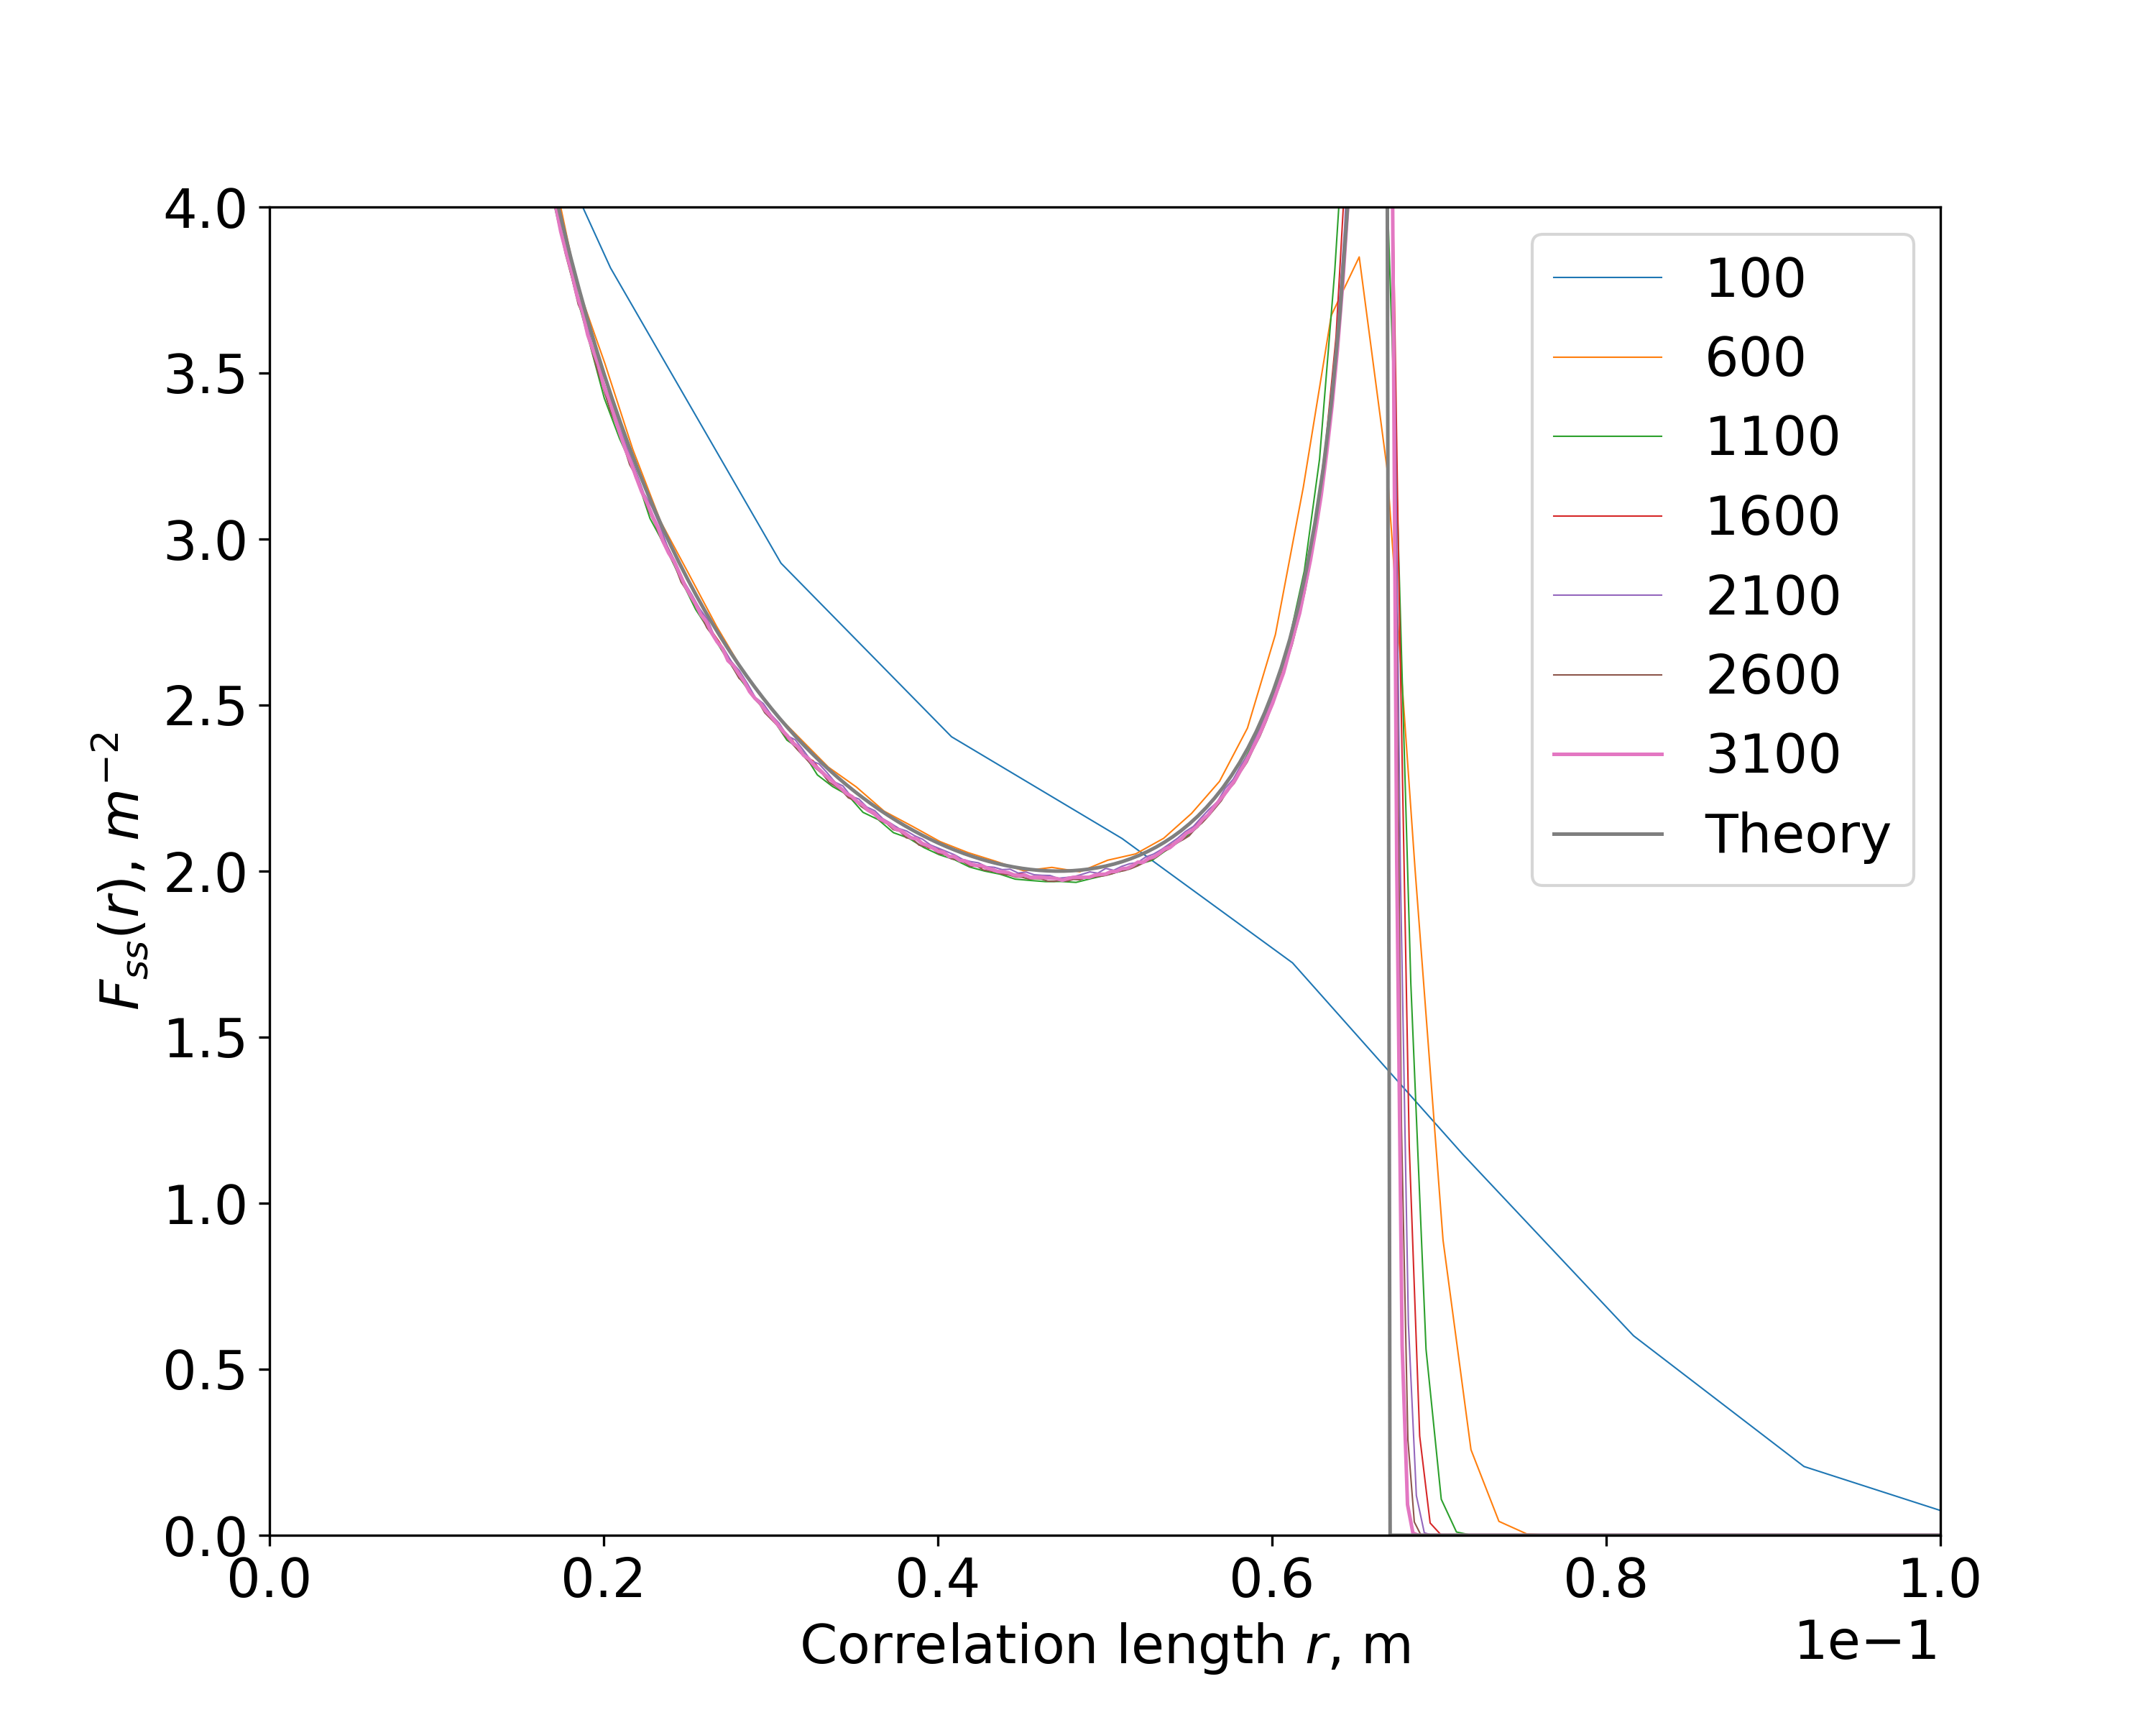
\includegraphics[width=0.45\linewidth]{images/fss-disk-5x5.png}
    \label{fig:fss-disk-5x5}}
  \caption[]{Plot of surface-surface function for a disk with radius
    $R = 0.334$. Resolution of the image varies from $100\times 100$ pixels to
    $3100\times 3100$.}
  \label{fig:fss-disk}
\end{figure*}

If $\bm{x} \in \mathbb{R}^3$ then an inequation $f(\bm{x}) \le R^2$ defines a
ball. In this case we provide a comparison (\cref{fig:fsss-ball}) of the
algorithm in \cref{sec:algo} with the precise algorithm in
\cref{sec:fsss-3d}. There is no known analytic solution for this case.
\begin{figure*}[!hpt]
  \centering
  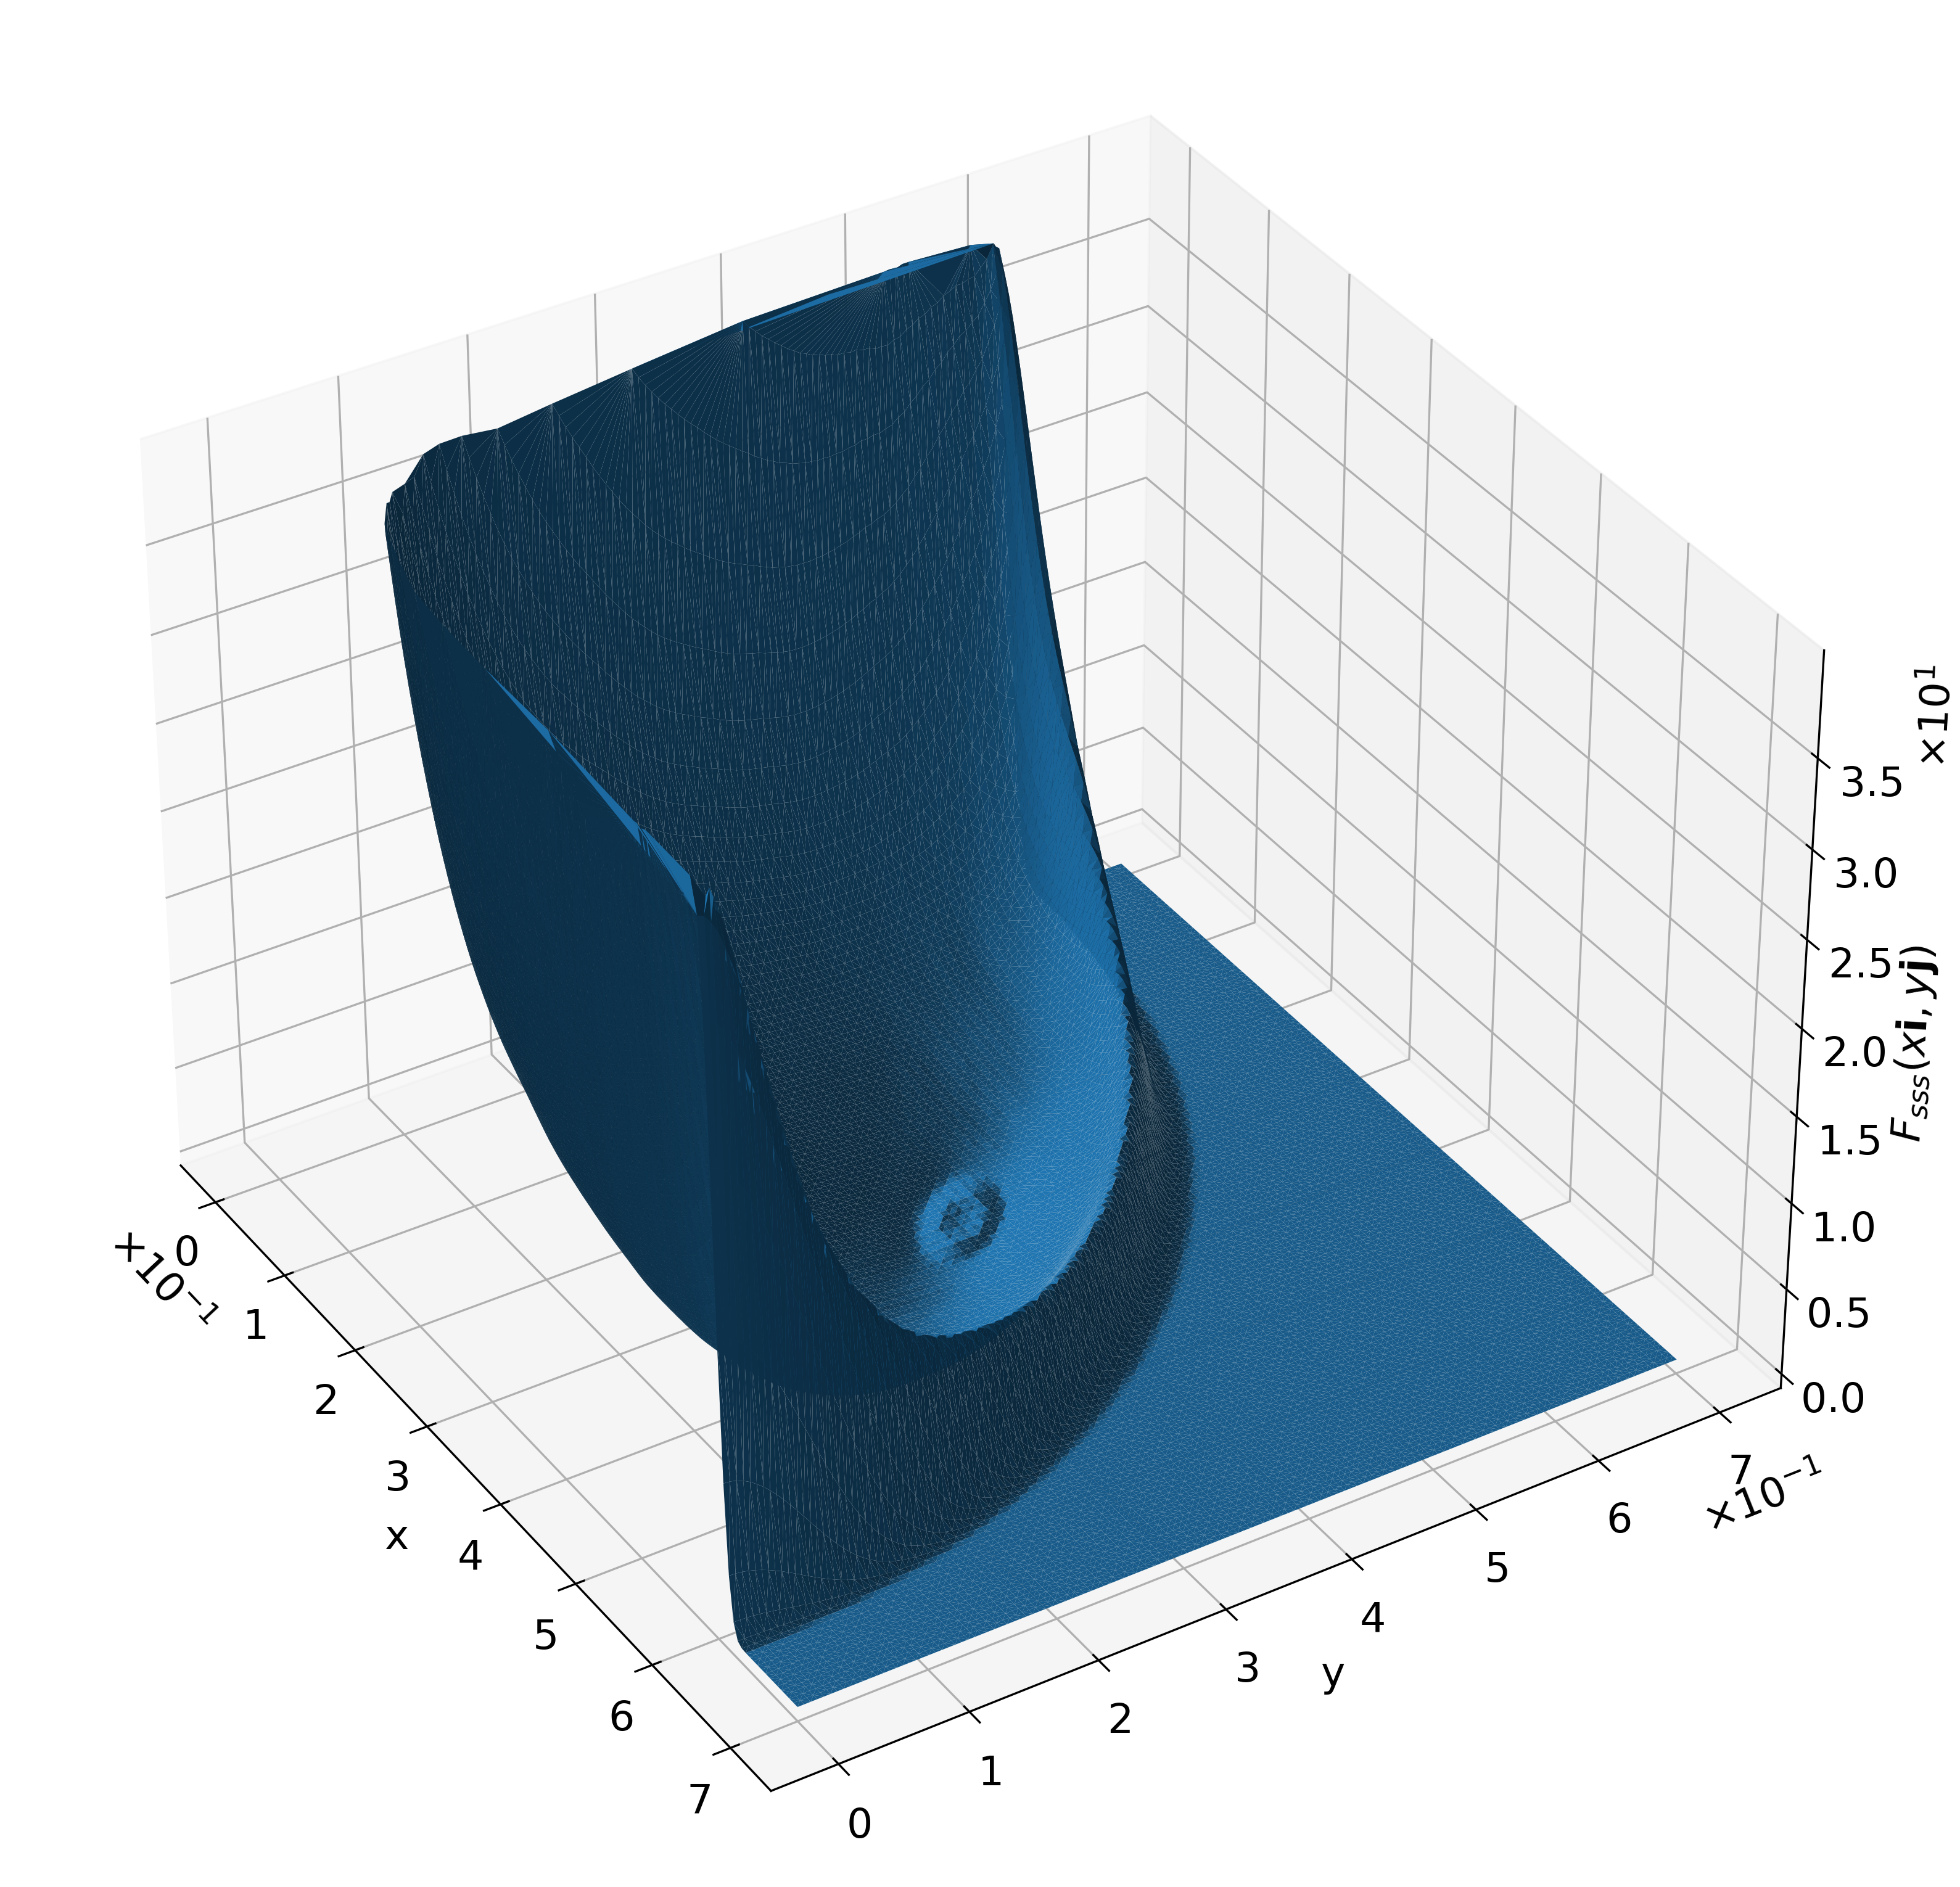
\includegraphics[width=0.45\linewidth]{images/ball-sss.png}
  \hfill
  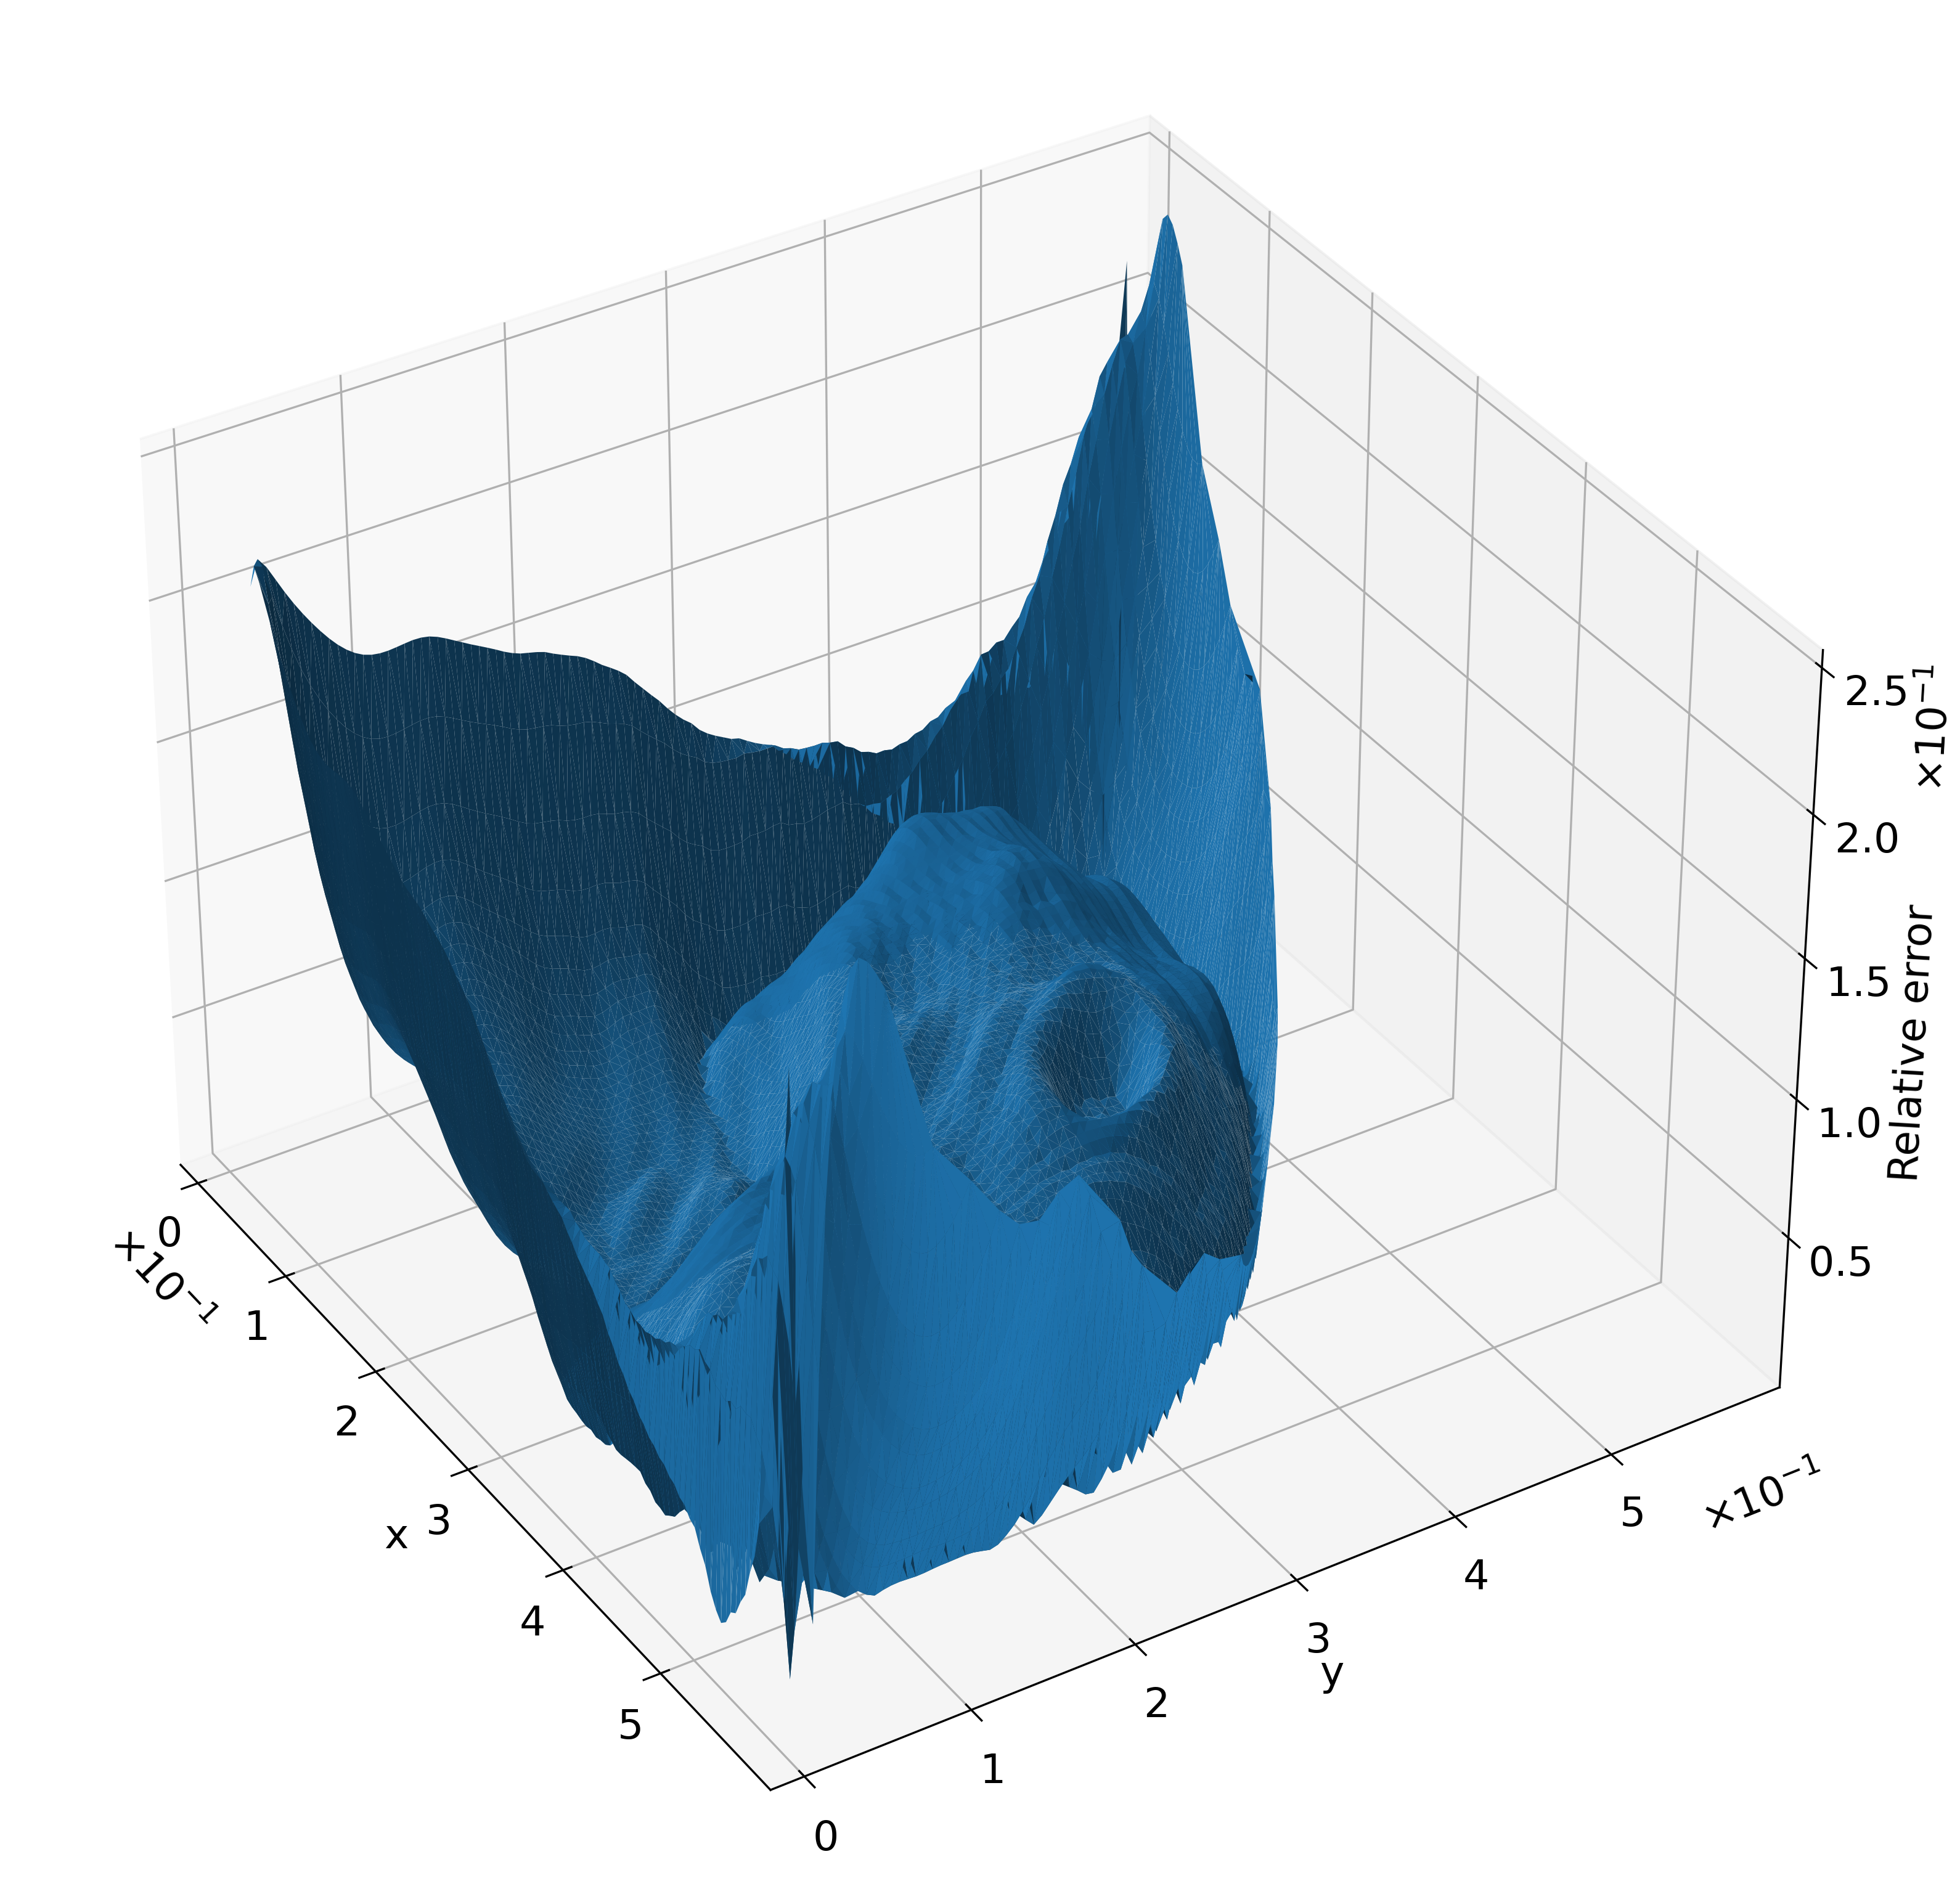
\includegraphics[width=0.45\linewidth]{images/ball-sss-error.png}
  \caption[]{On the left: Plot of $F_{sss}(\bm{r_1}, \bm{r_2})$ function
    obtained by algorithm \cref{sec:algo} for a ball with radius
    $R = 0.3$. $\bm{r_1}$ is parallel to a vector $\bm{i} = (1, 0, 0)$ and
    $\bm{r_2}$ is parallel to a vector $\bm{j} = (0, 1, 0)$. Vectors $\bm{i}$
    and $\bm{j}$ constitute a two dimensional parameter space for $F_{sss}$. On
    the right: Relative error of computation. True values for $F_{sss}$ are
    obtained by algorithm in \cref{sec:fsss-3d}.}
  \label{fig:fsss-ball}
\end{figure*}

\subsection{Gaussian mixture}
\label{sec:gauss}
\begin{figure}
  \centering
  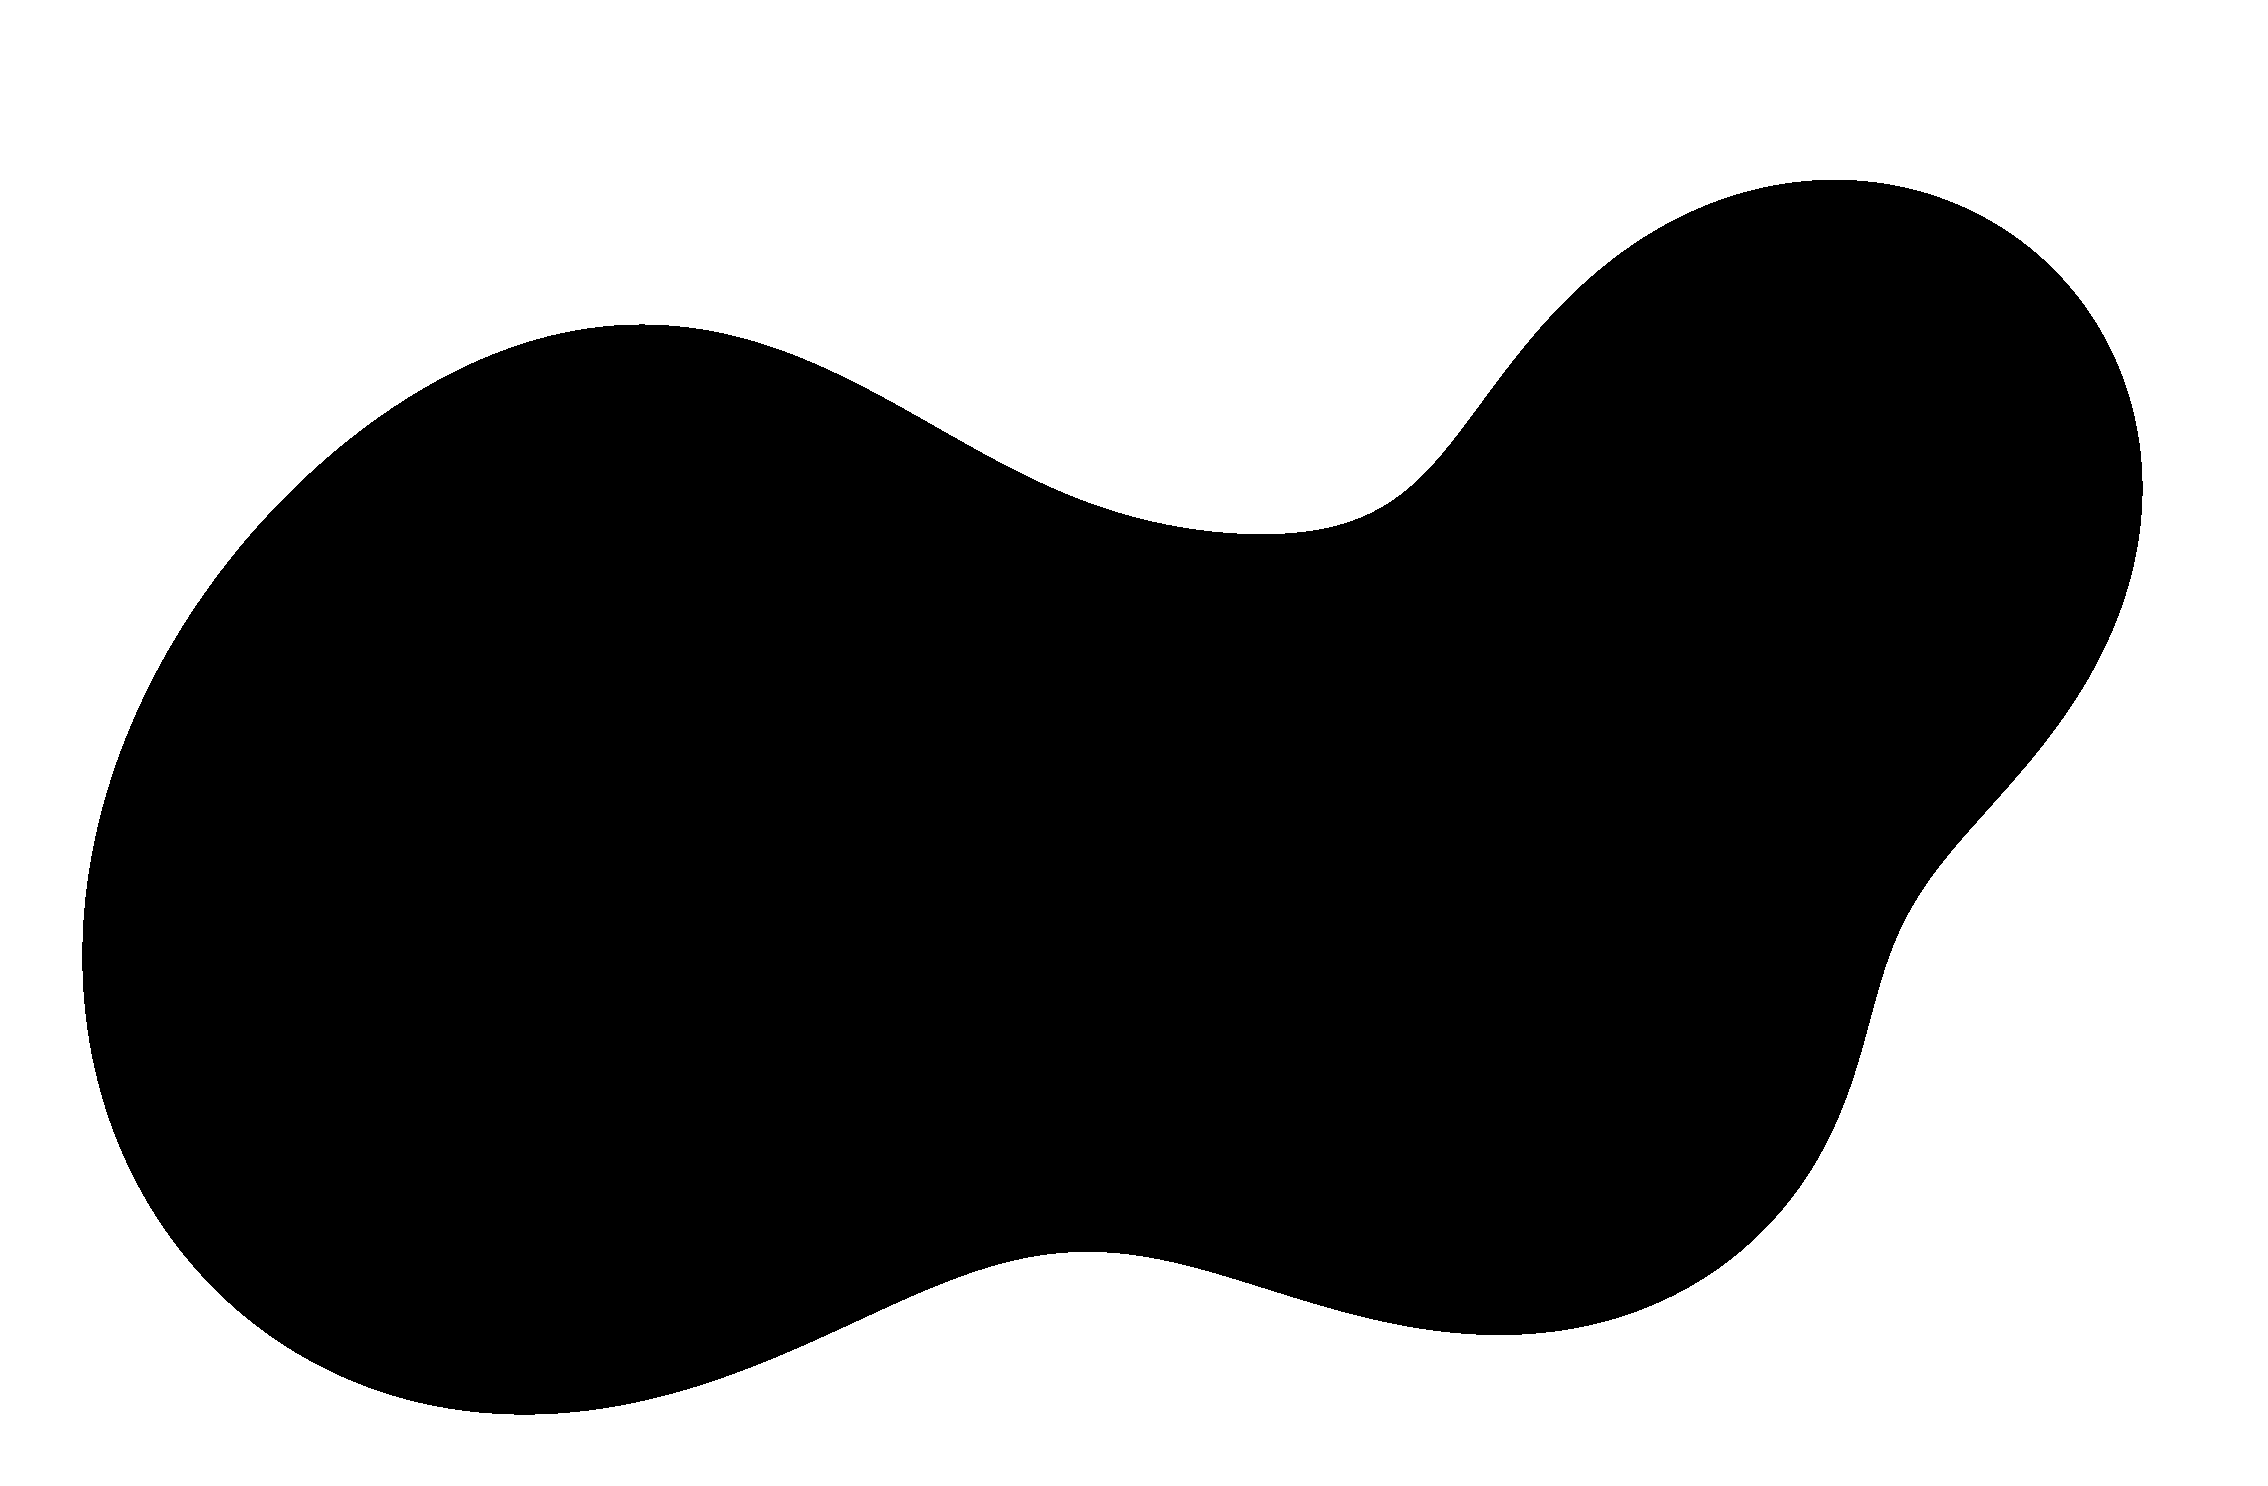
\includegraphics[width=0.8\linewidth, frame]{images/blob.png}
  \caption[]{An example of a ``blob'' generated by Gaussian mixture $f(x,y)$
    which consists of four Gaussian functions. White area is where
    $f(x,y) \le 3$.}
  \label{fig:blob}
\end{figure}
Take $N$ random values $a_i$, $b_i$ and $\sigma_i$. Let $f$ be
\begin{equation*}
  f(x,y) = \sum_{i=1}^N \frac{1}{\sigma_i} \exp(\frac{-(x-a_i)^2-(y-b_i)^2}{\sigma_i^2})
\end{equation*}
Inequality $f(x,y) \le T$ defines a ``blob'' like one which can be seen on
\cref{fig:blob}. We can use the algorithm developed in \cref{sec:fss-2d} to
compute precise values of $F_{ss}$ for this blob and compare them with values
obtained by using the algorithm in section \cref{sec:algo}. The result of this
comparison is on \cref{fig:fss-blob}.
\begin{figure*}[!hpt]
  \centering
  \subfigure[$3\times 3$ kernel $H$]{
    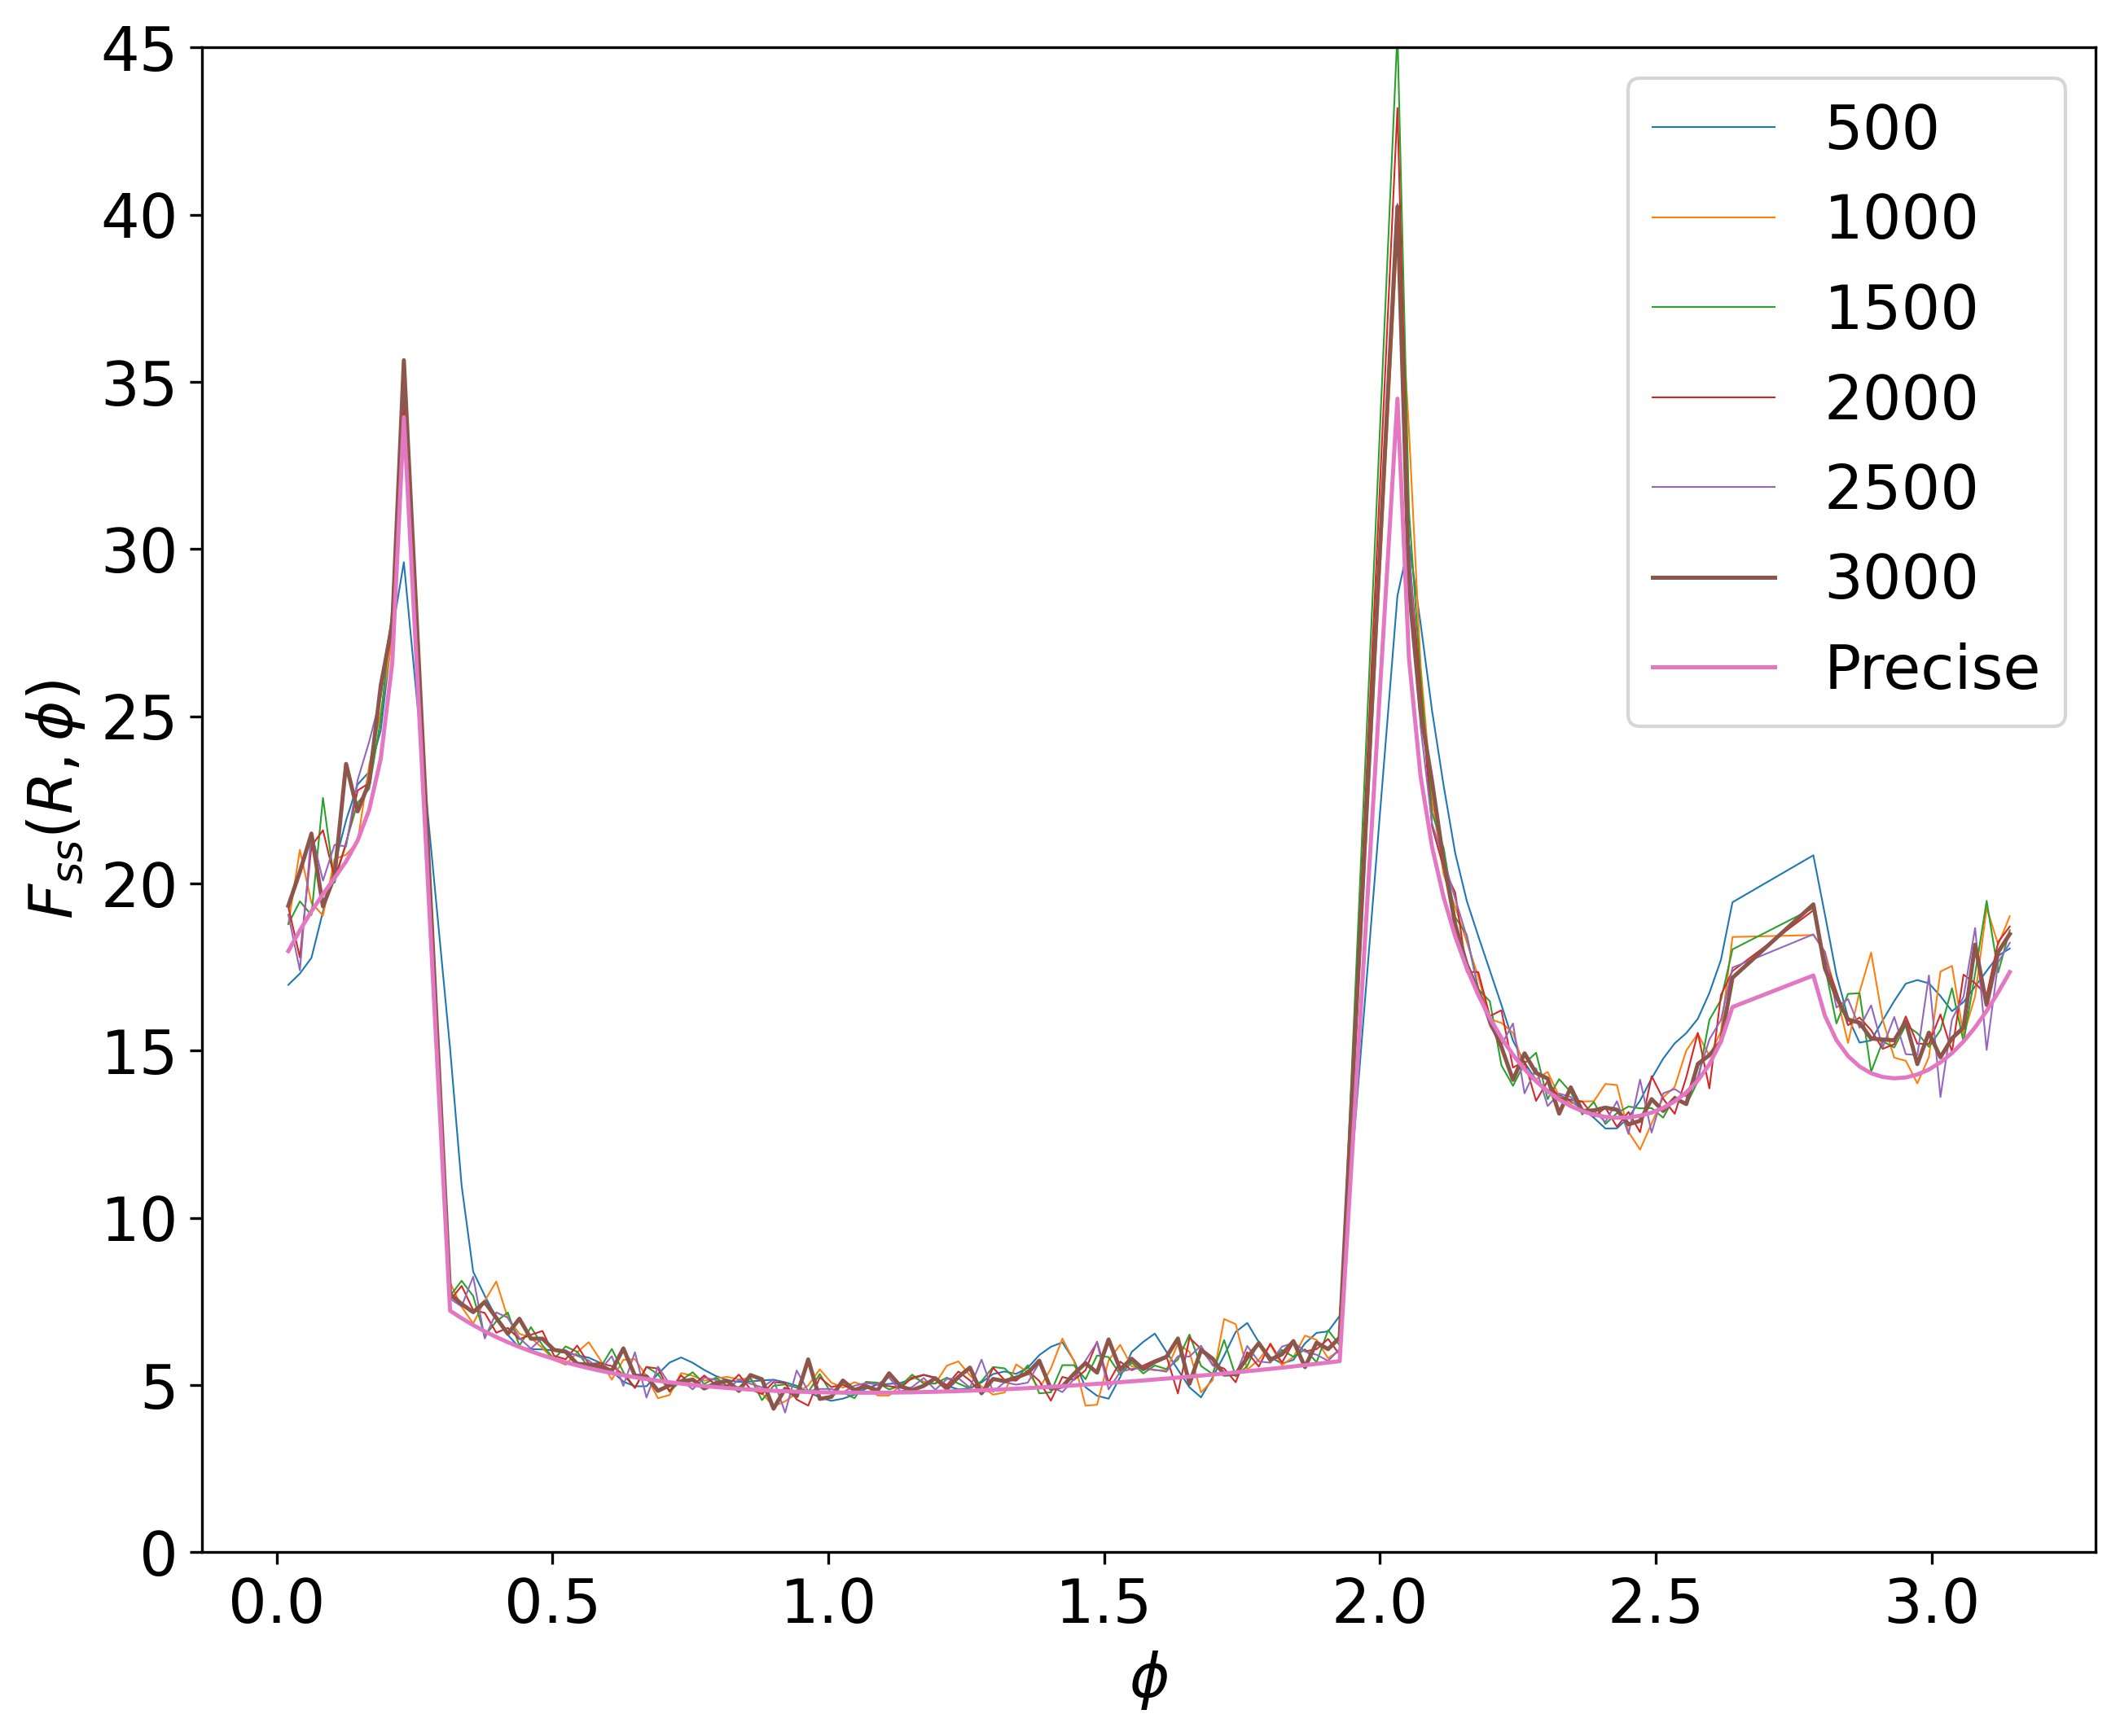
\includegraphics[width=0.45\linewidth]{images/fss-blob-3x3.png}
    \label{fig:fss-blob-3x3}}
  \hfill
  \subfigure[$5\times 5$ kernel $H'$]{
    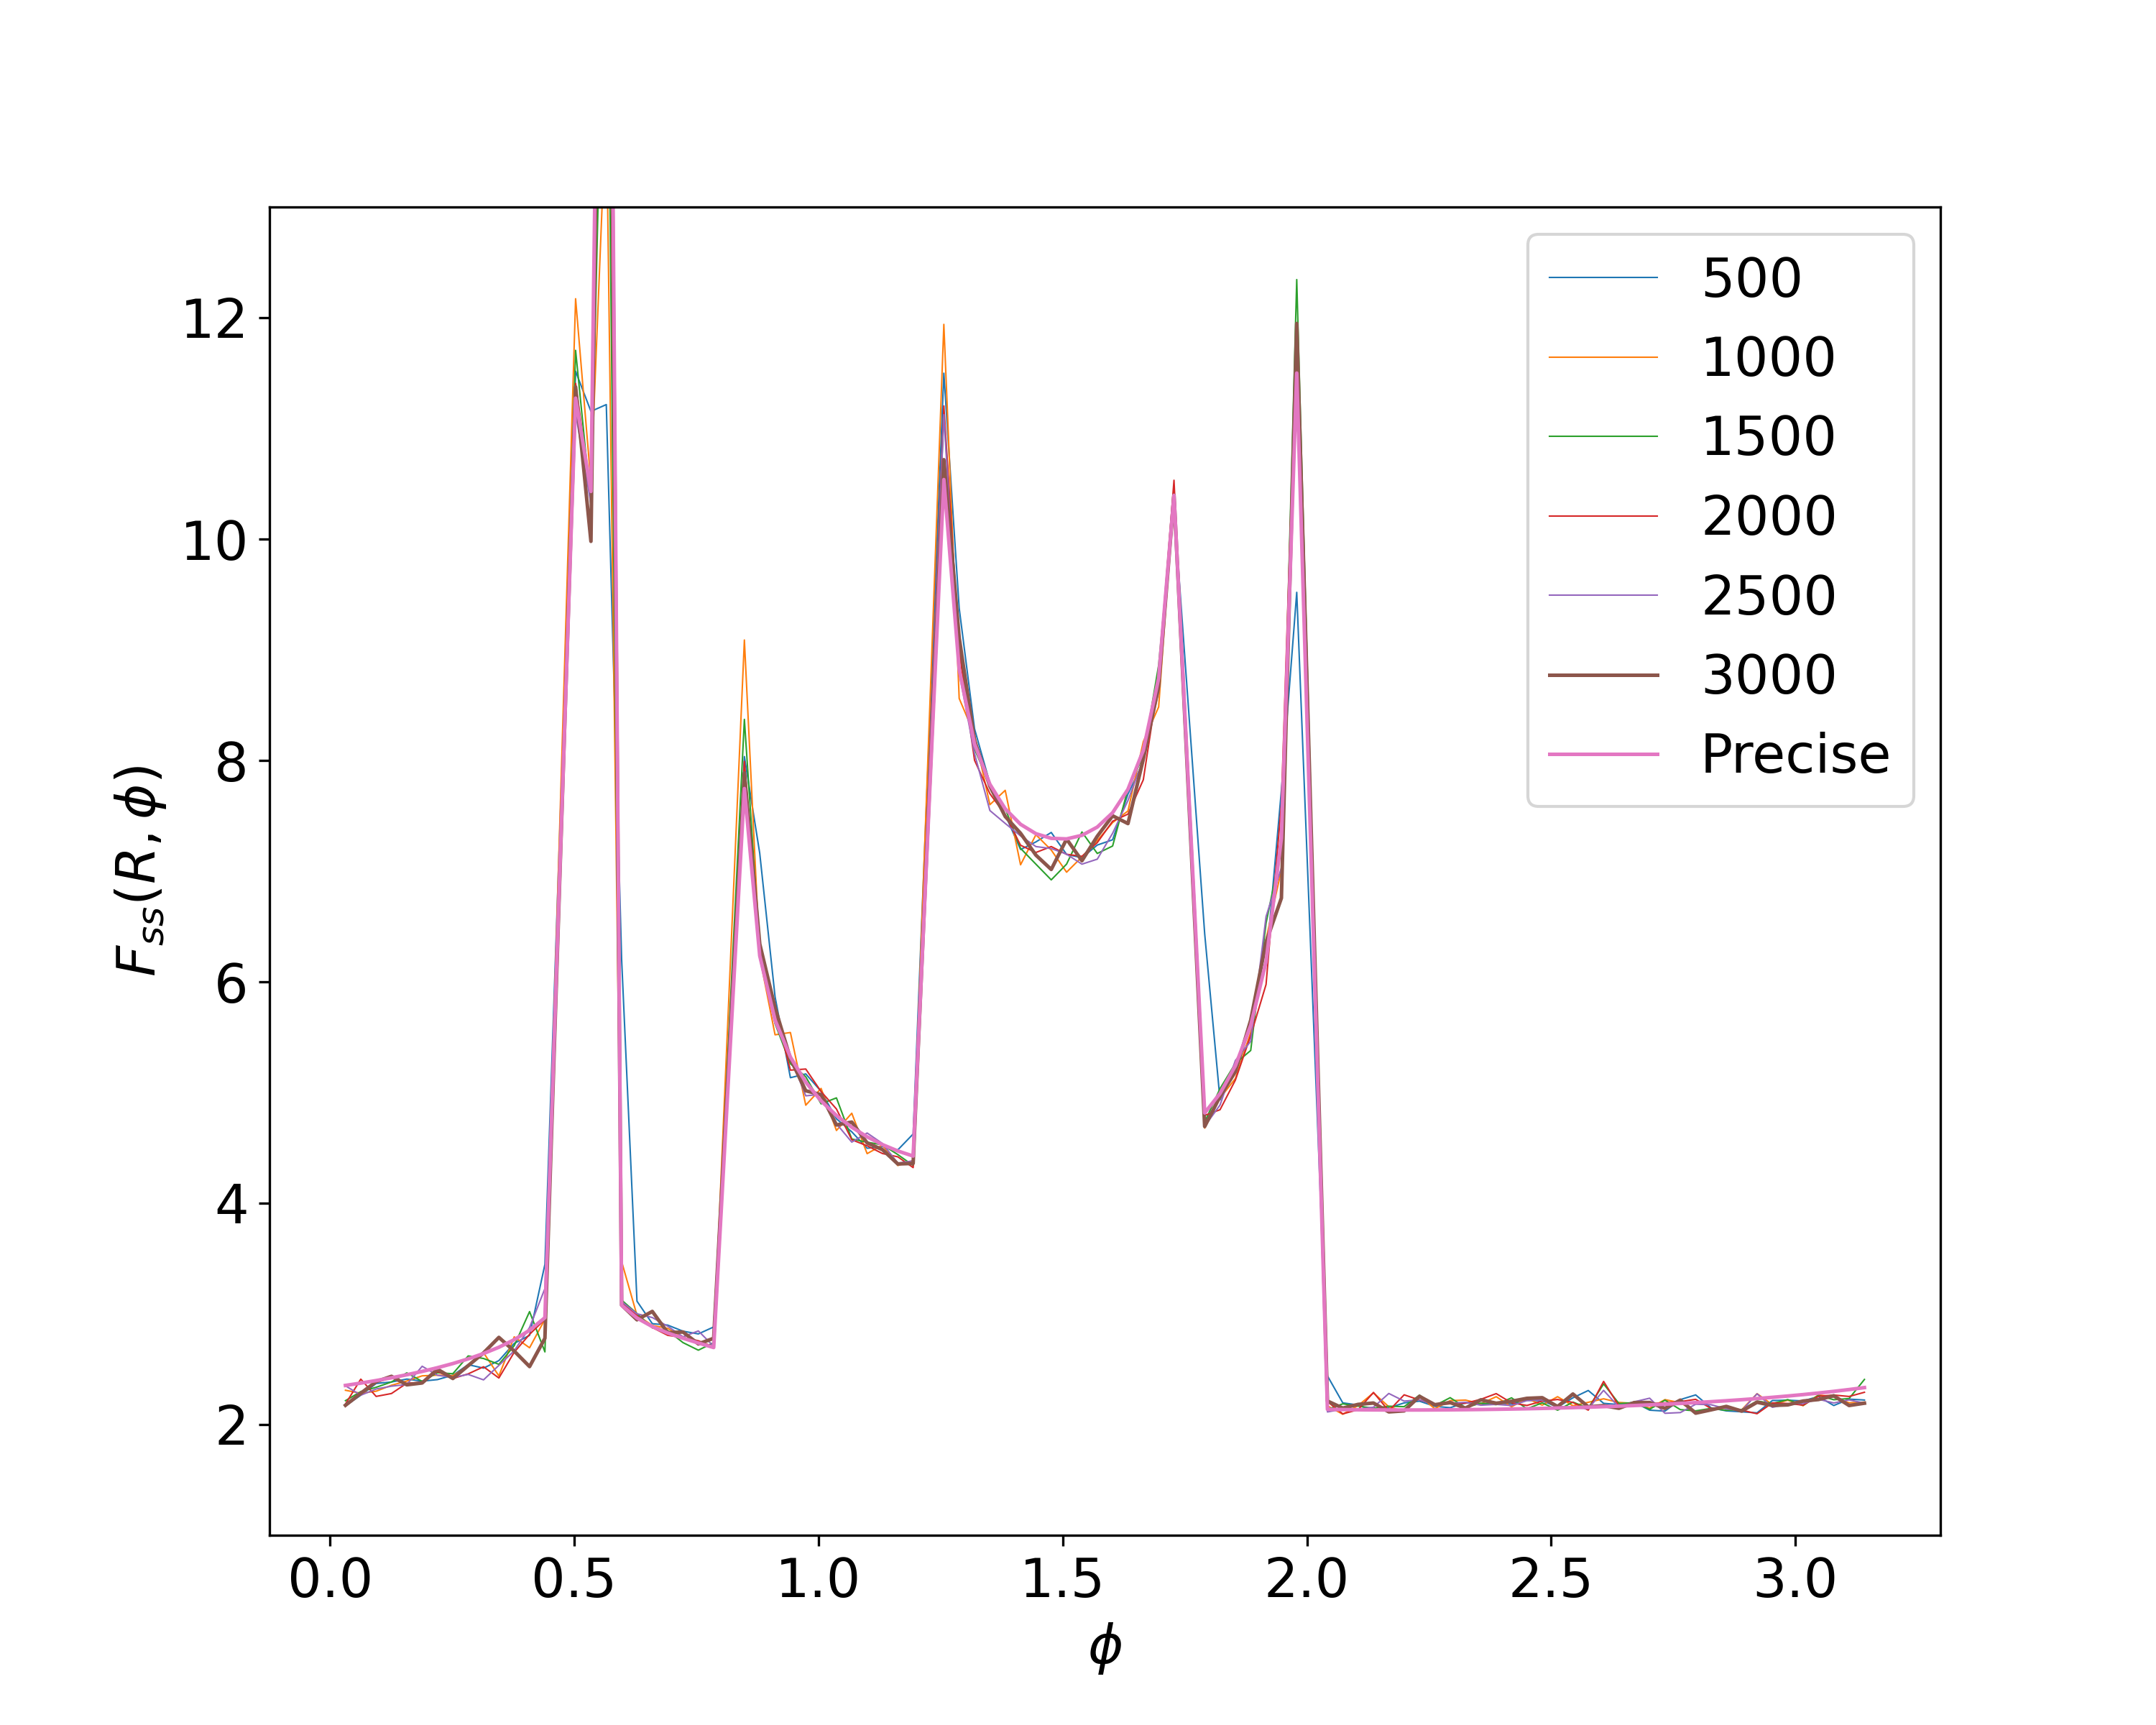
\includegraphics[width=0.45\linewidth]{images/fss-blob-5x5.png}
    \label{fig:fss-blob-5x5}}
  \caption[]{Plot of the surface-surface function for the blob on
    \cref{fig:blob}. Values of $F_{ss}$ were calculated in semi-circle with
    radius $R = 0.3$ and angle $\phi$ varying from $0$ to $\pi$. Resolution of
    the image varies from $500\times 500$ pixels to $3000\times 3000$.}
  \label{fig:fss-blob}
\end{figure*}

\subsection{Ellipses}
\label{sec:ellipses}
\begin{figure}
  \centering
  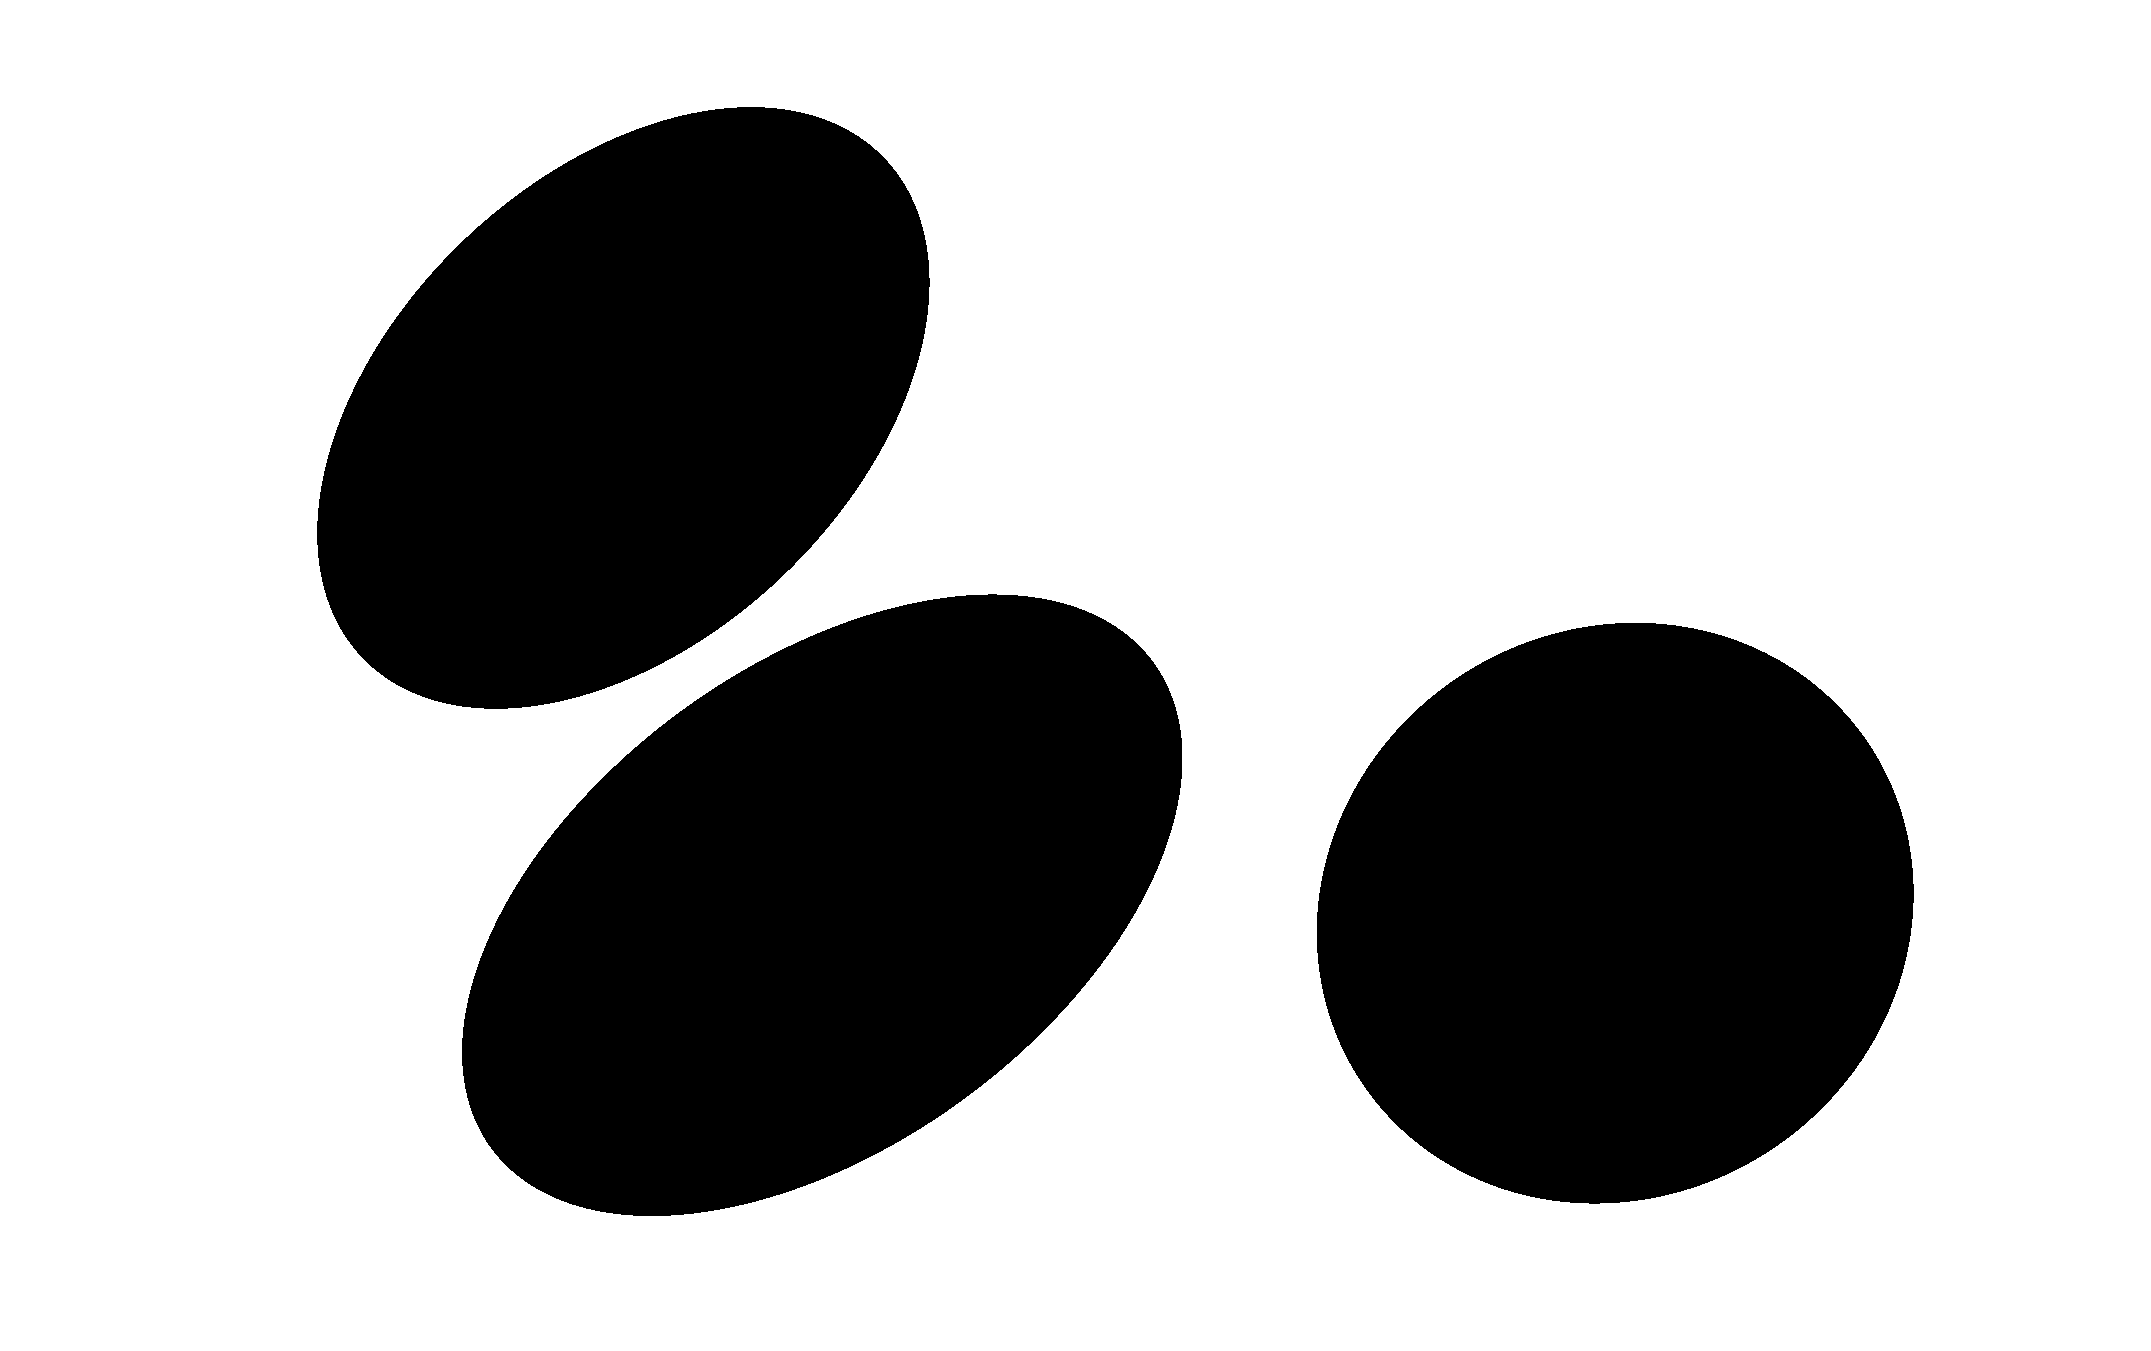
\includegraphics[width=0.8\linewidth, frame]{images/ellipses.png}
  \caption[]{An example of generated ellipses.}
  \label{fig:ellipses}
\end{figure}
Take $N$ random values $a_i$, $b_i$, $c_i$, $x^c_i$ and $y^c_i$ and define
\begin{equation*}
  f_i(x, y) = a_i(x-x^c_i)^2 + b(x-x^c_i)(y-y^c_i) + c_i(y-y^c_i)^2
\end{equation*}
with $a_ic_i - b_i^2 > 0$. Inequation
\begin{equation*}
  \min_i f_i(x, y) < A^2
\end{equation*}
defines $N$ ellipses like those which can be seen on \cref{fig:ellipses}. A
comparison between two algorithms is on \cref{fig:fss-ellipses}.
\begin{figure*}[!hpt]
  \centering
  \subfigure[$3\times 3$ kernel $H$]{
    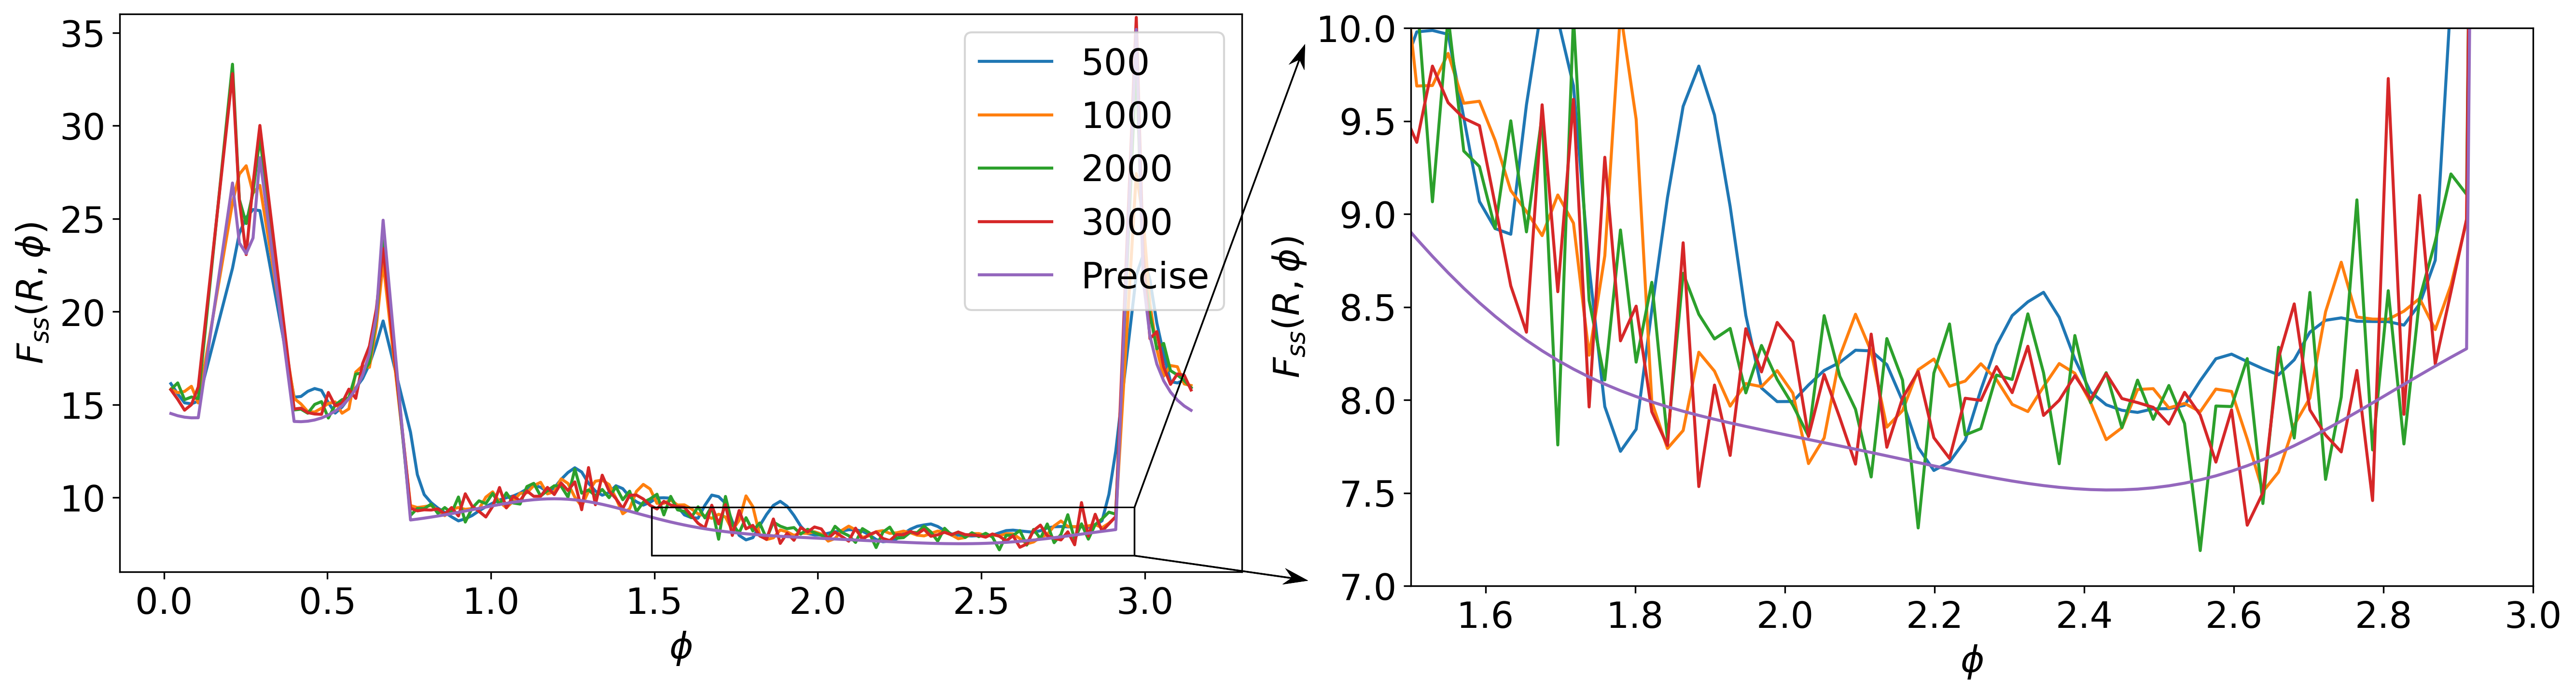
\includegraphics[width=0.45\linewidth]{images/fss-ellipses-3x3.png}
    \label{fig:fss-ellipses-3x3}}
  \hfill
  \subfigure[$5\times 5$ kernel $H'$]{
    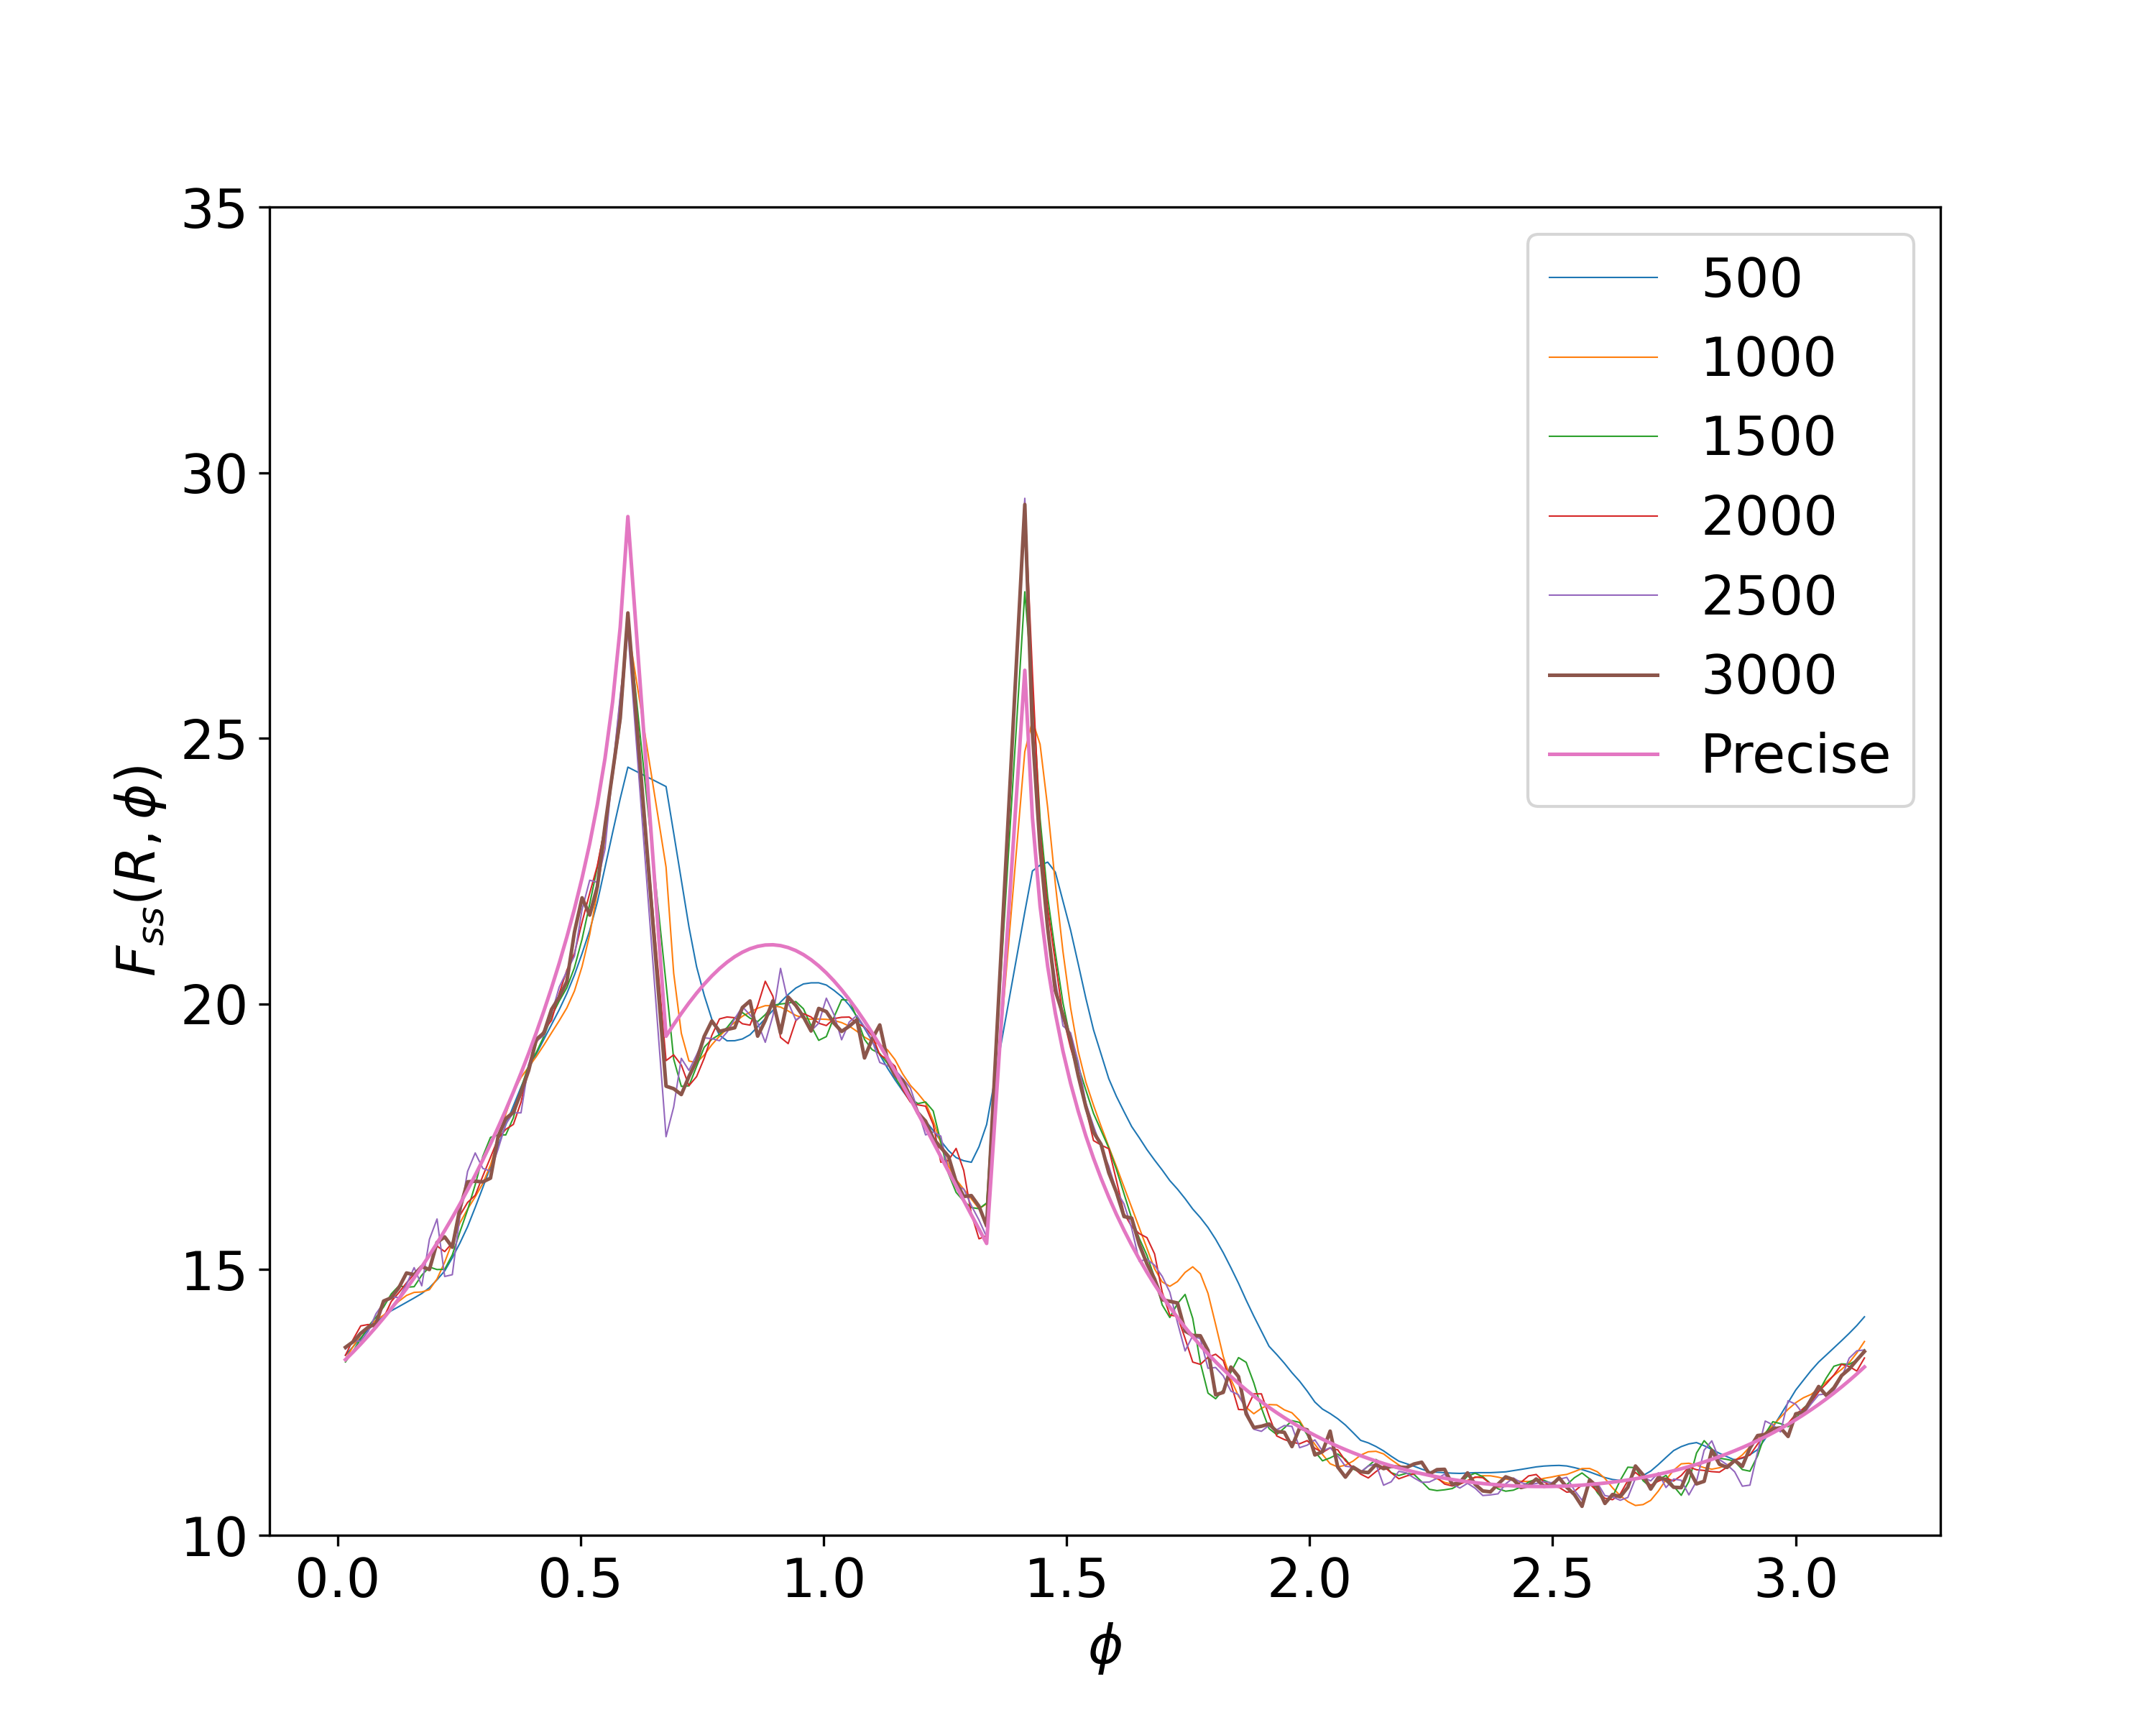
\includegraphics[width=0.45\linewidth]{images/fss-ellipses-5x5.png}
    \label{fig:fss-ellipses-5x5}}
  \caption[]{Plot of the surface-surface function for ellipses on
    \cref{fig:ellipses}. Values of $F_{ss}$ were calculated in semi-circle with
    radius $R = 0.1$ and angle $\phi$ varying from $0$ to $\pi$. Resolution of
    the image varies from $500\times 500$ pixels to $3000\times 3000$.}
  \label{fig:fss-ellipses}
\end{figure*}

\subsection{Influence of filter $H'$ on cases not covered by the new algorithm}
In this section we show how filter $H'$ affects calculation of surface-functions
in cases not covered by the algorithm described in \cref{sec:fss-2d} and
\cref{sec:fsss-3d}.

\begin{figure*}
  \centering
  \subfigure[Surface-surface function calculated for a ball with radius
    $R = 0.24$. Image dimensions are  $450 \times 450 \times 450$.]{
    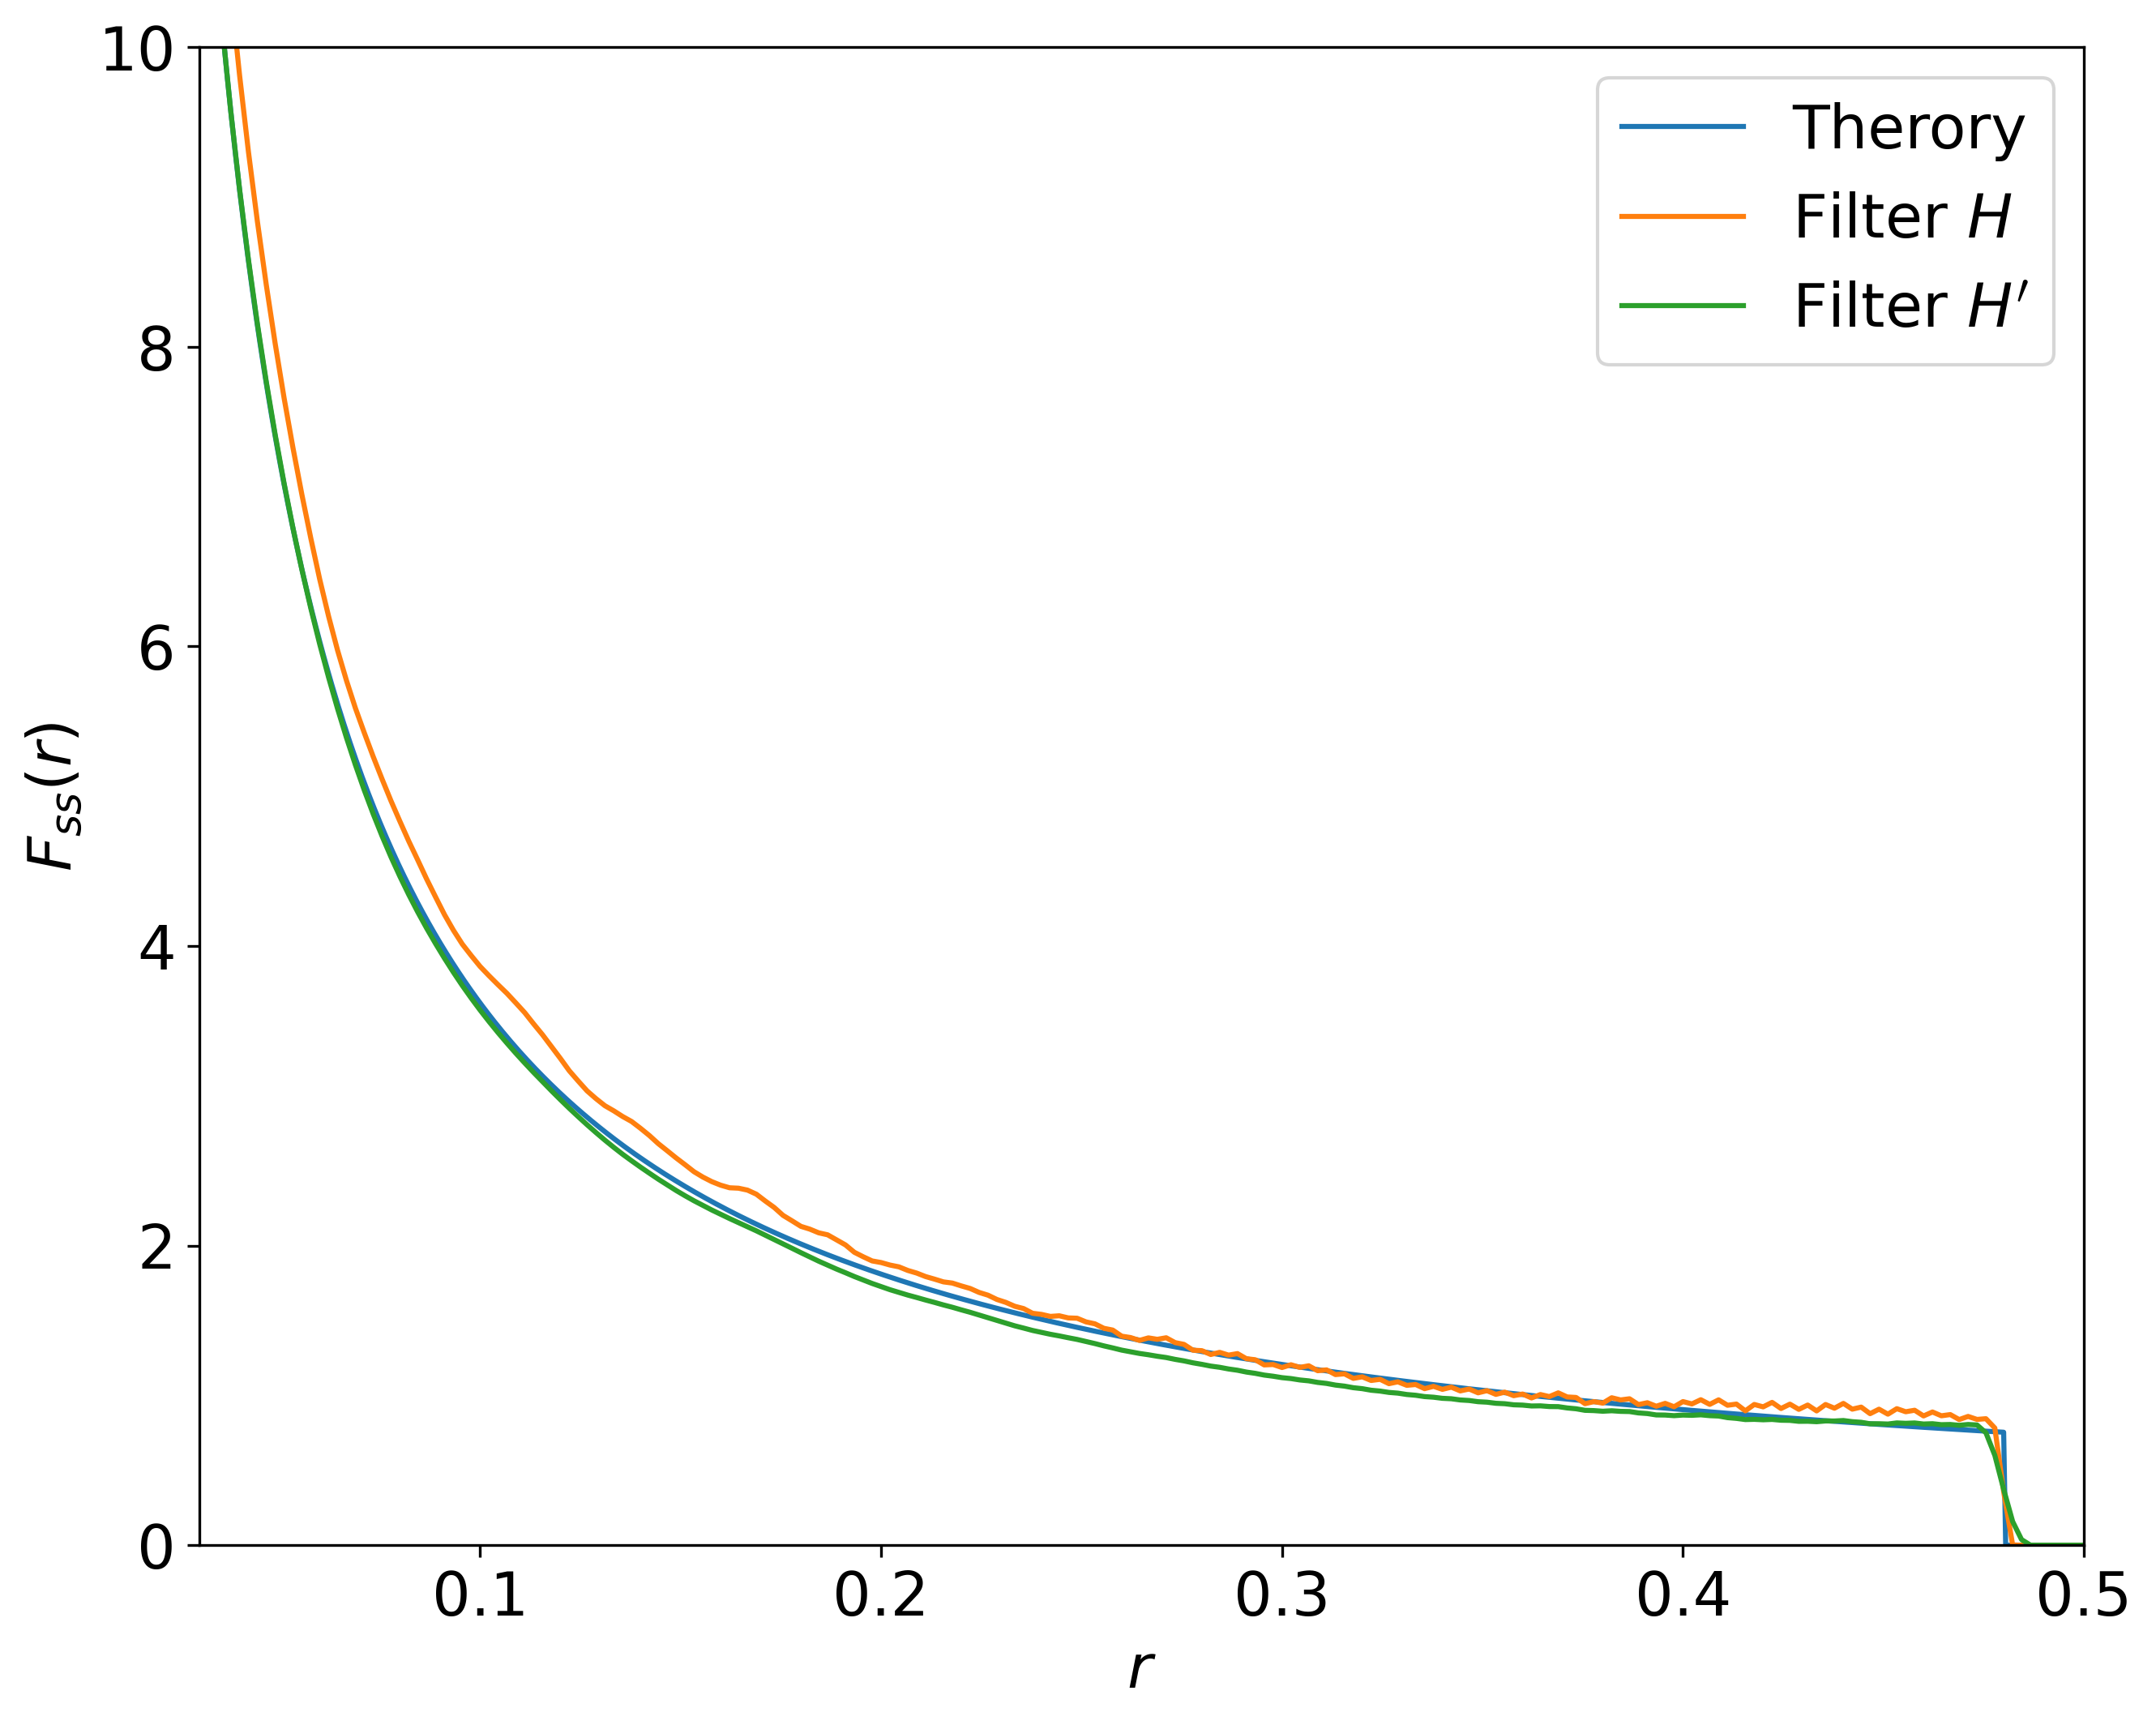
\includegraphics[width=0.3\linewidth]{images/ball-3d-ss.png}
    \label{fig:fss-ball}}
  \hfill
  \subfigure[Surface-void function calculated for a disk with radius
    $R = 0.2$. Image dimensions are $2000 \times 2000$.]{
    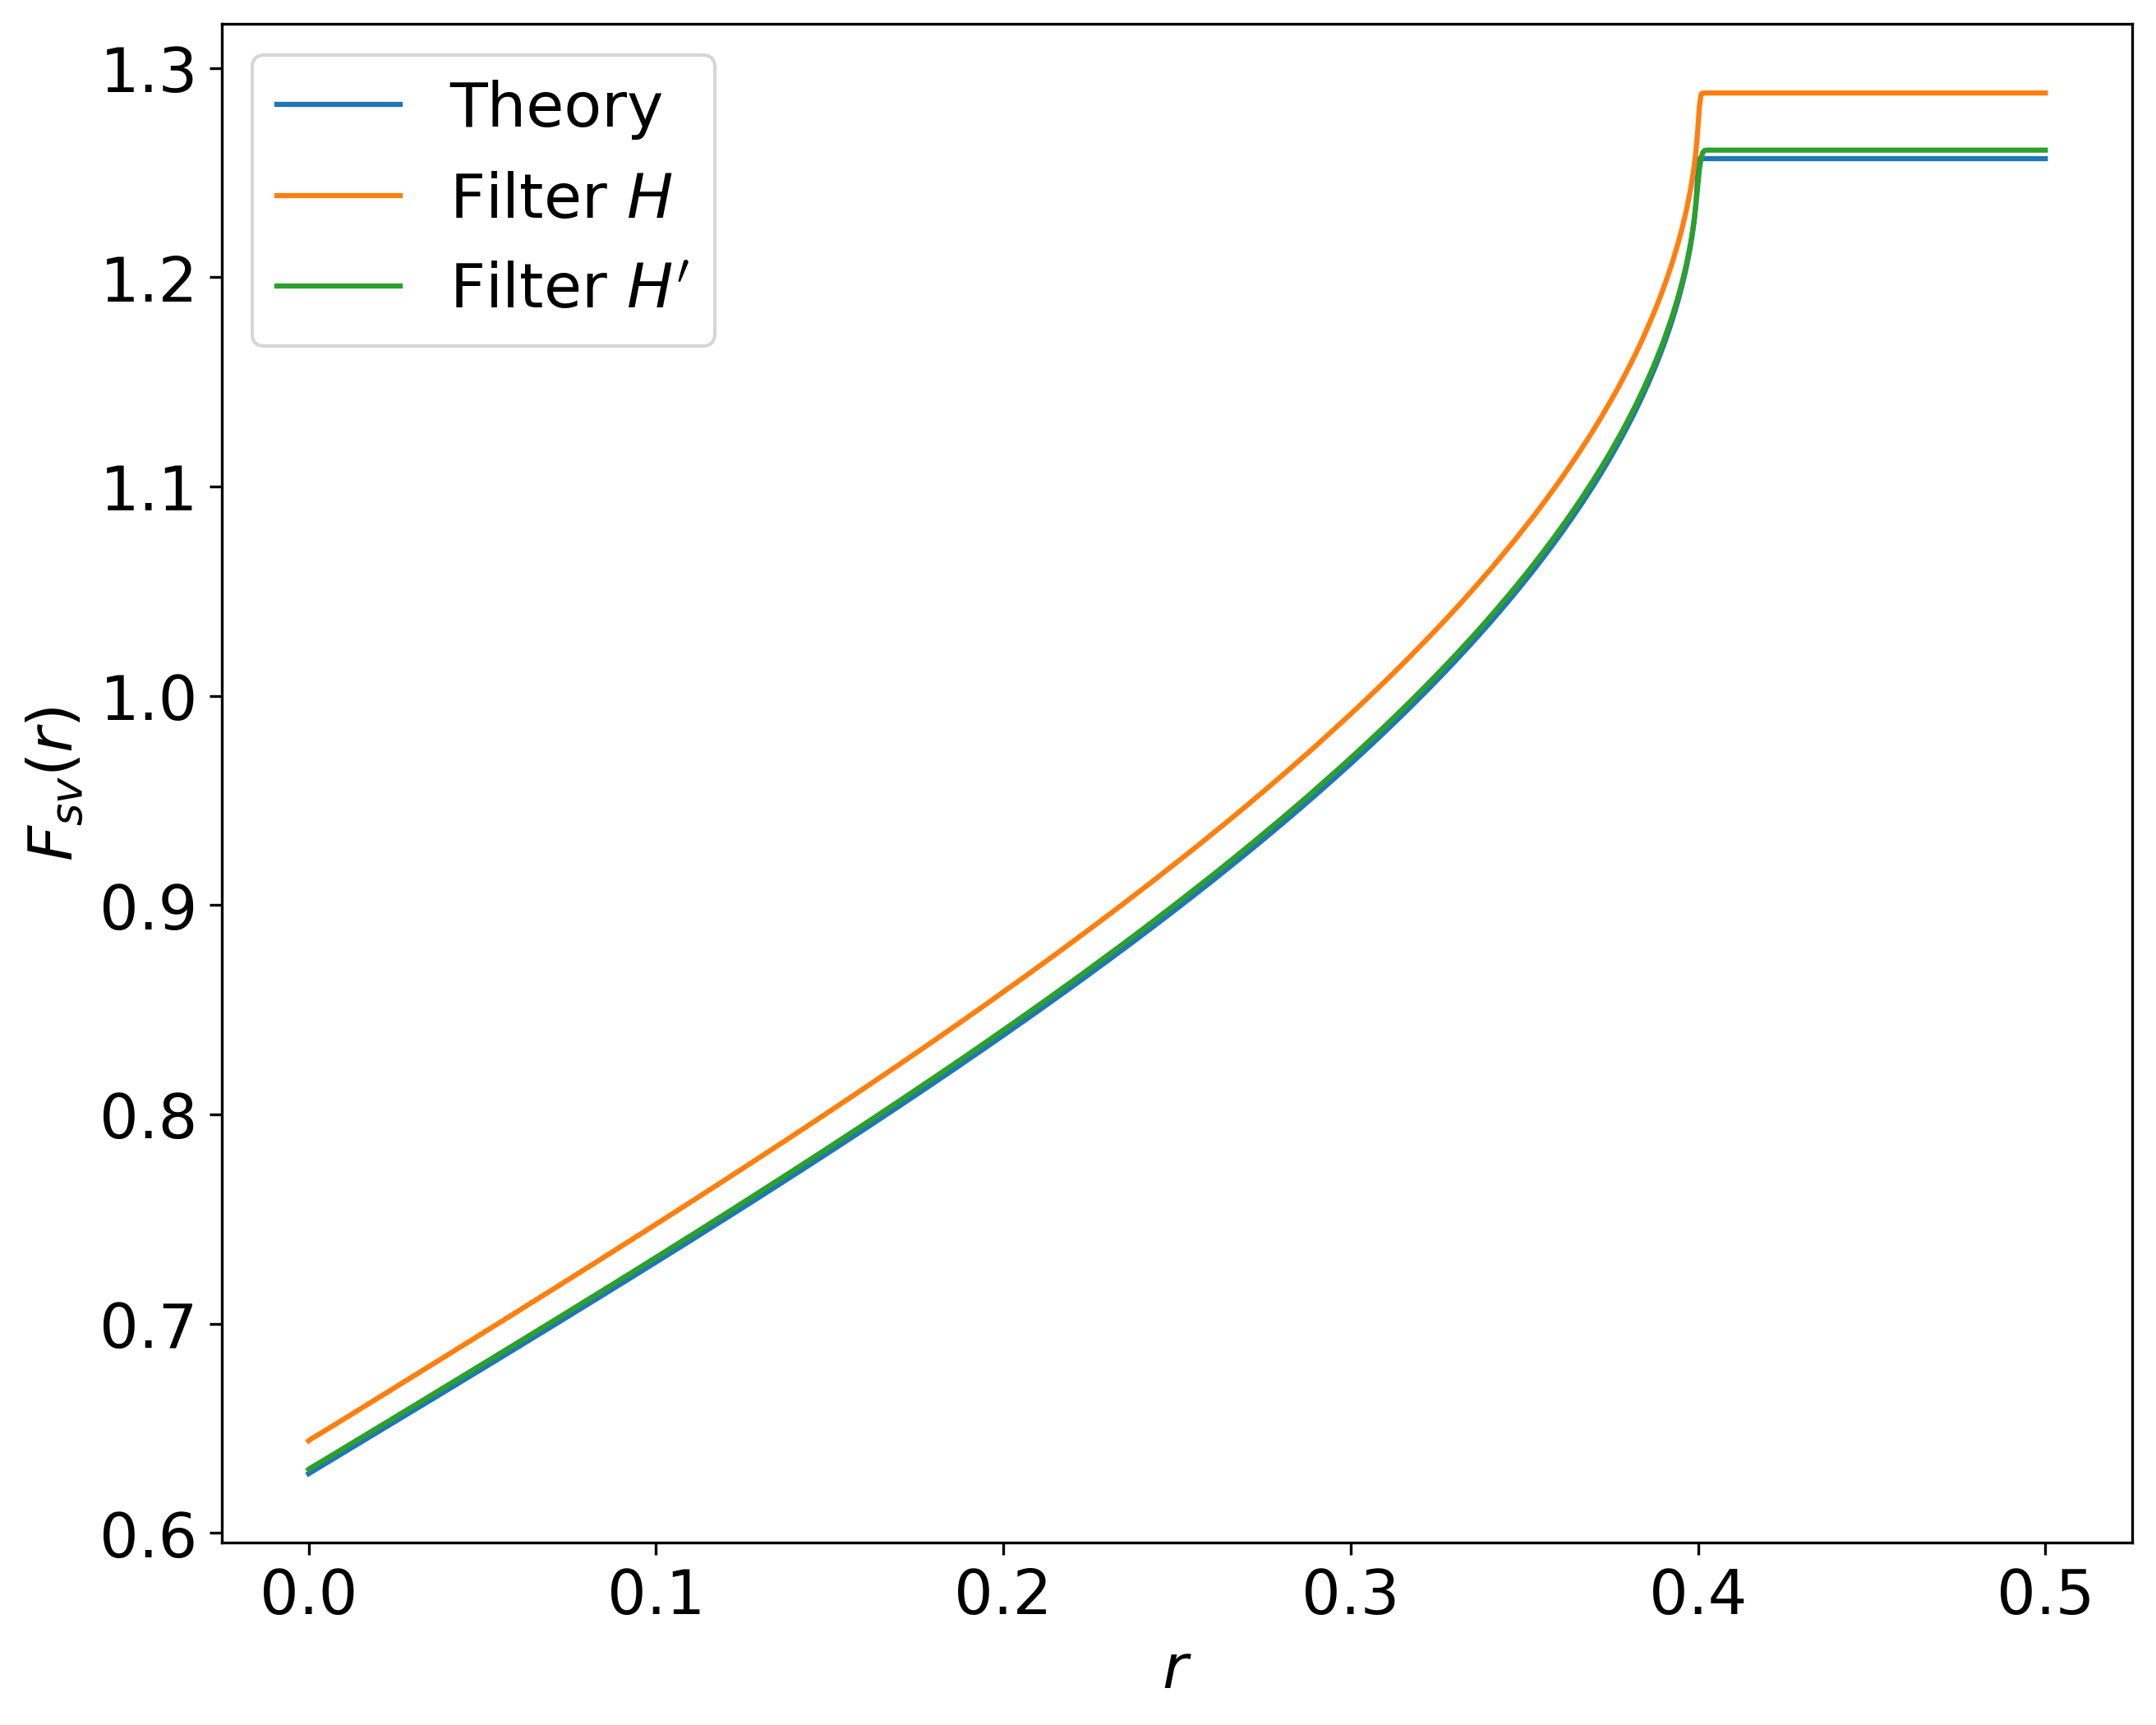
\includegraphics[width=0.3\linewidth]{images/fsv-disk.png}
    \label{fig:fsv-disk}}
  \hfill
  \subfigure[Surface-void function calculated for a ball with radius
    $R = 0.2$. Image dimensions are $300 \times 300 \times 300$.]{
    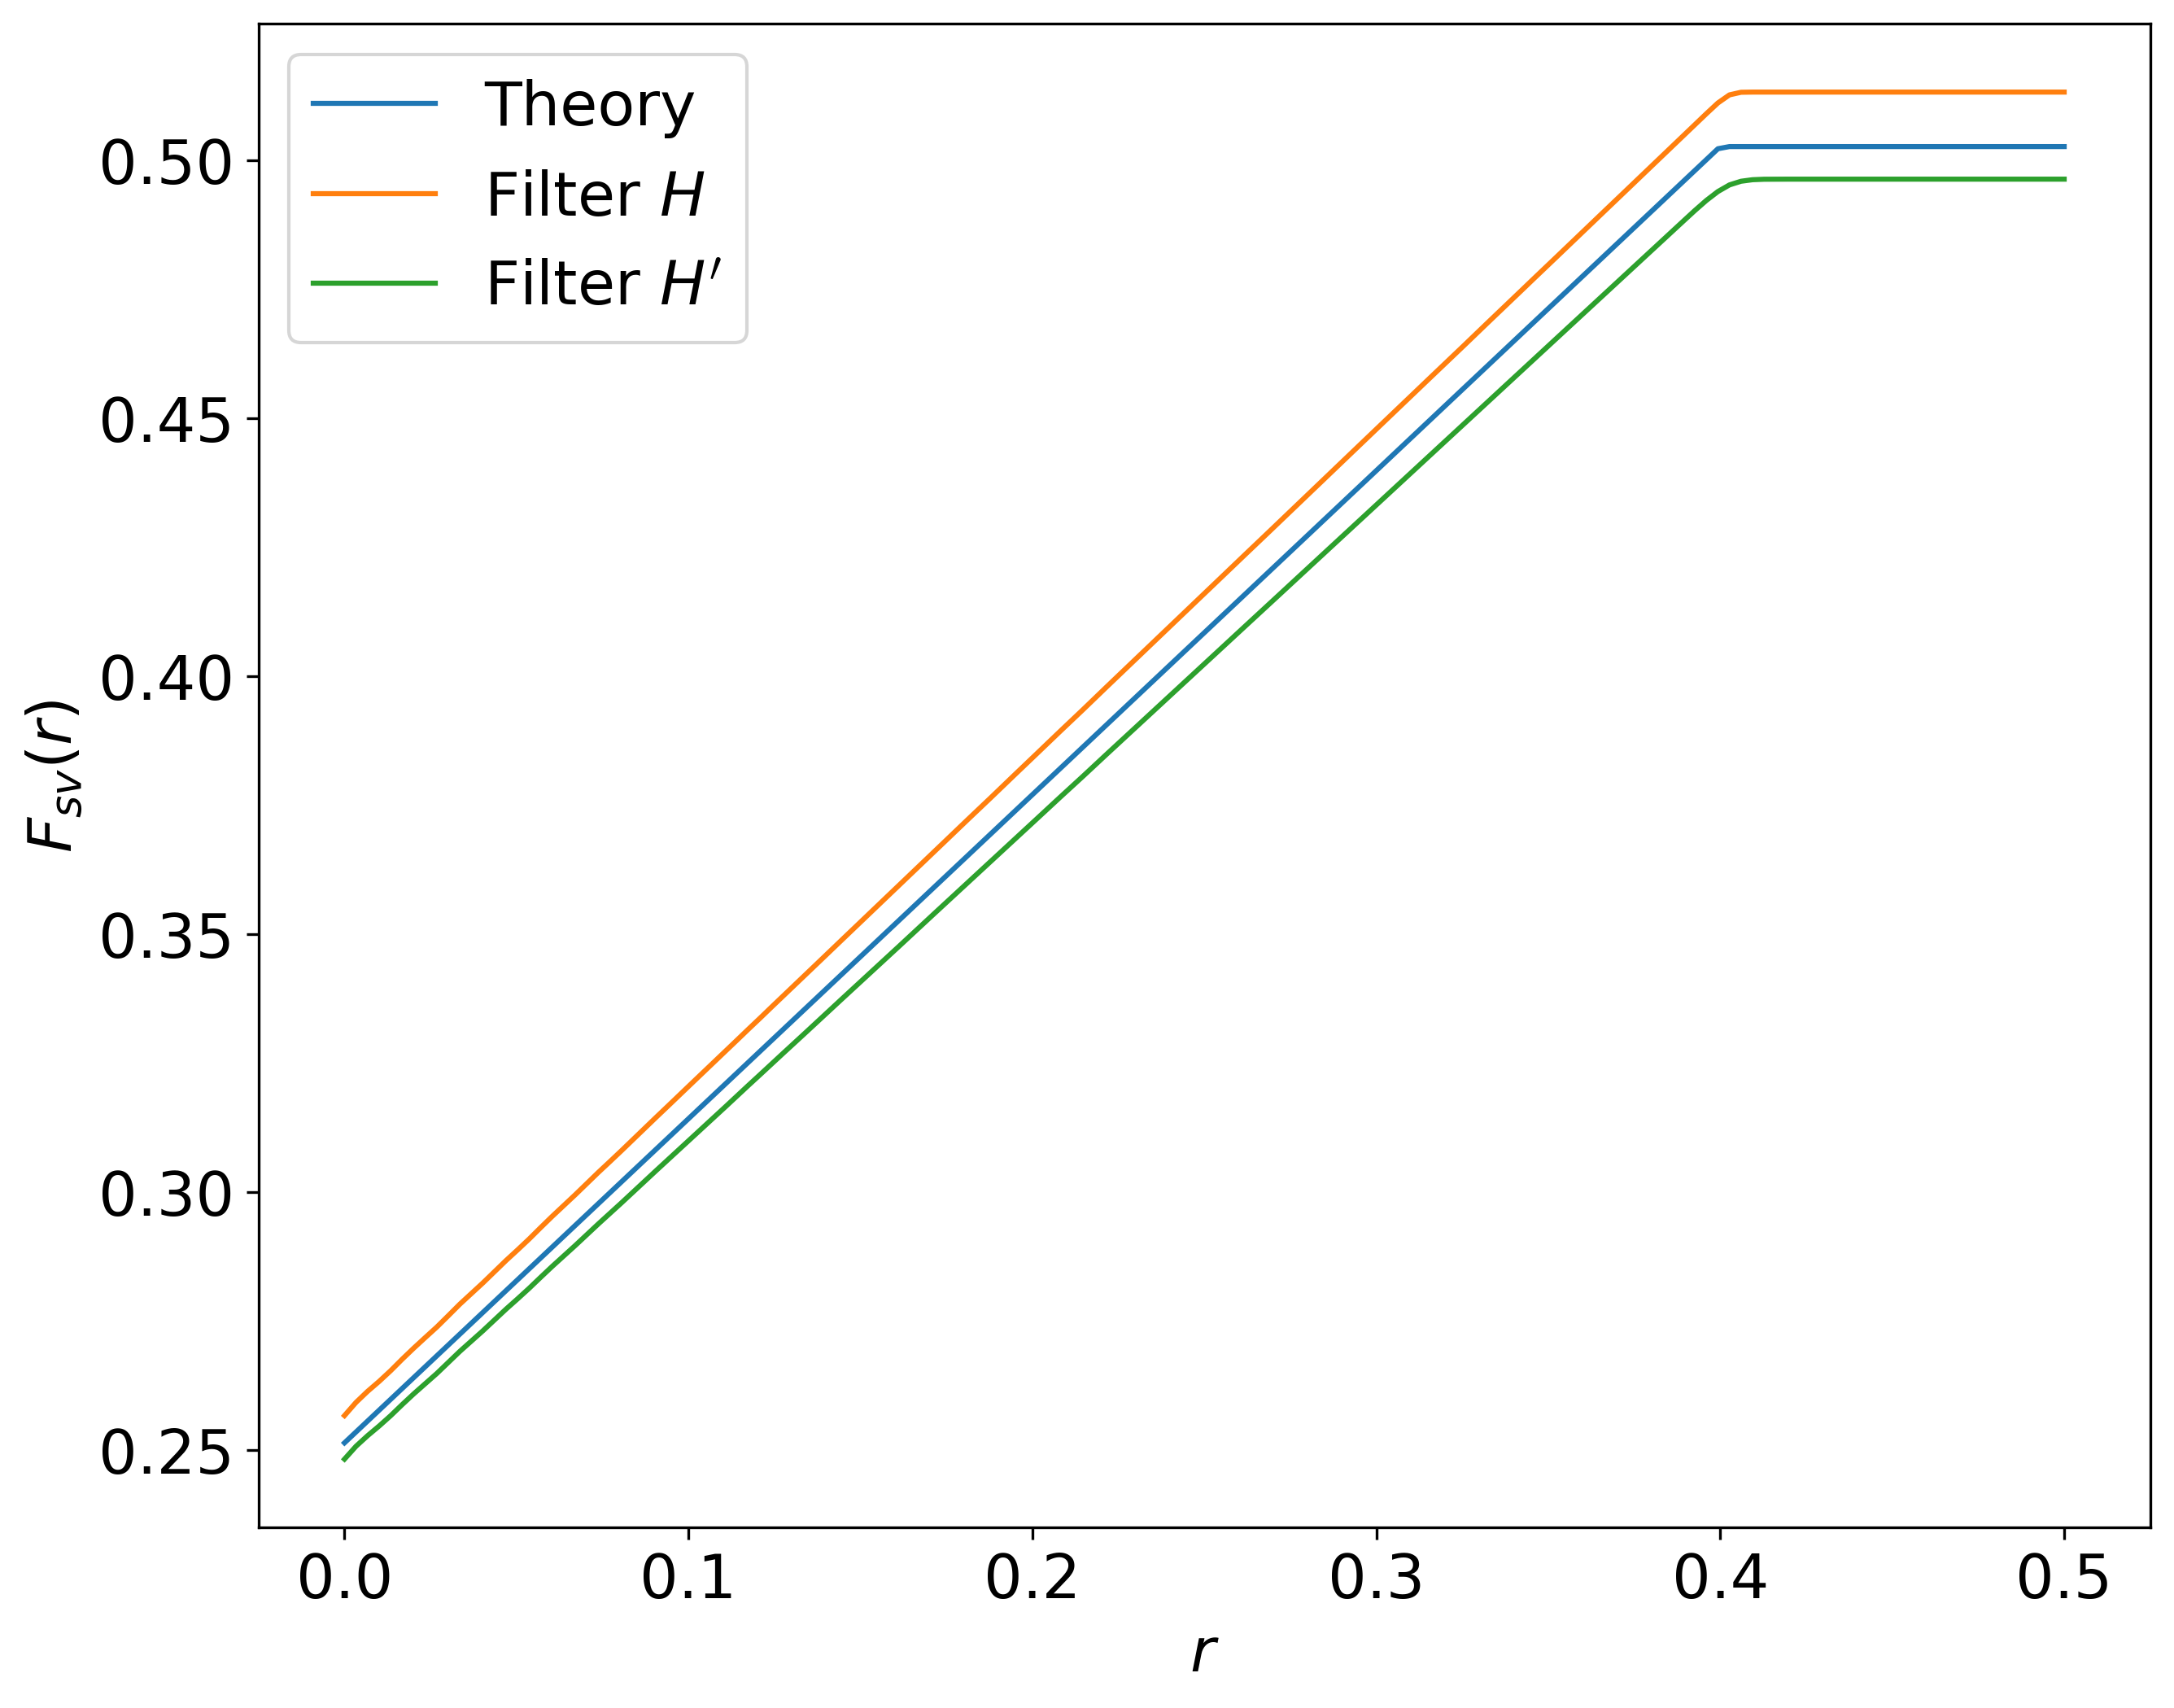
\includegraphics[width=0.3\linewidth]{images/fsv-ball.png}
    \label{fig:fsv-ball}}
  \caption[]{Comparison of filters $H$ and $H'$ for cases in which newly
    developed algorithms \cref{sec:fss-2d}, \cref{sec:fsss-3d} are not
    applicable. Theoretical curves are provided for each case.}
  \label{fig:not-covered}
\end{figure*}
With the new filter calculation of $F_{ss}$ becomes more precise also for
three-dimensional images. This can be seen in comparison with theoretical values
for known cases like the one of a ball. On \cref{fig:fss-ball} there are plots
of $F_{ss}$ function calculated with filters $H$ and $H'$ along with a
theoretical curve. It can be verified that filter $H'$ is better indeed by
calculating
\begin{equation*}
  error = \sqrt{\frac{\sum_i (F_{ss}^{calc}(x_i) -
      F_{ss}^{theory}(x_i))^2}{\sum_i F_{ss}^{theory}(x_i)^2}}
\end{equation*}
where $x_i$ belong to a set
$(\epsilon, 2R - \epsilon) \cup (2R + \epsilon, 1)$. Taking $\epsilon = 0.01$ we
get $error = 0.006$ for filter $H$ and $error = 0.00017$ for filter
$H'$. Calculation of surface-void function also benefits from the new filter
(\cref{fig:fsv-disk}, \cref{fig:fsv-ball}).

Unfortunately the filter $H'$ has some drawbacks in comparison with $H$. Firstly
$H$ has faster convergence with increase of image resolution. Our
acceptance criterion developed in \textcolor{red}{cite our paper again} works
also for $H'$, but sometimes it's possible to calculate a poor estimate of
$F_{ss}$ using $H$ but not $H'$. Secondly, $H'$ behaves worse that $H$ in points
of discontinuity of $F_{ss}$ as can be seen on \cref{fig:fss-disk}.

\section{Conclusion}
% Is this a right label?
\label{sec:summary}
In this paper we develop an algorithm for precise calculation of $F_{ss}$
function for two-dimensional sets and $F_{sss}$ function for three-dimensional
sets. These sets must have smooth boundary for the algorithm to be
applicable. With help of this algorithm we introduce some new test cases and
check our algorithm for digital images more thoroughly. The algorithm is
improved using a wider filter $H'$.

An implementation of the precise algorithm for sets with smooth boundary is
available on GitHub\cite{diff-boundary-corrfn}.

\bibliography{paper}
\end{document}
